\chapter{Pipeline bioinformático para el análisis de secuencias del gen 16S}

% \begin{figure}[H]
%     \centering
%     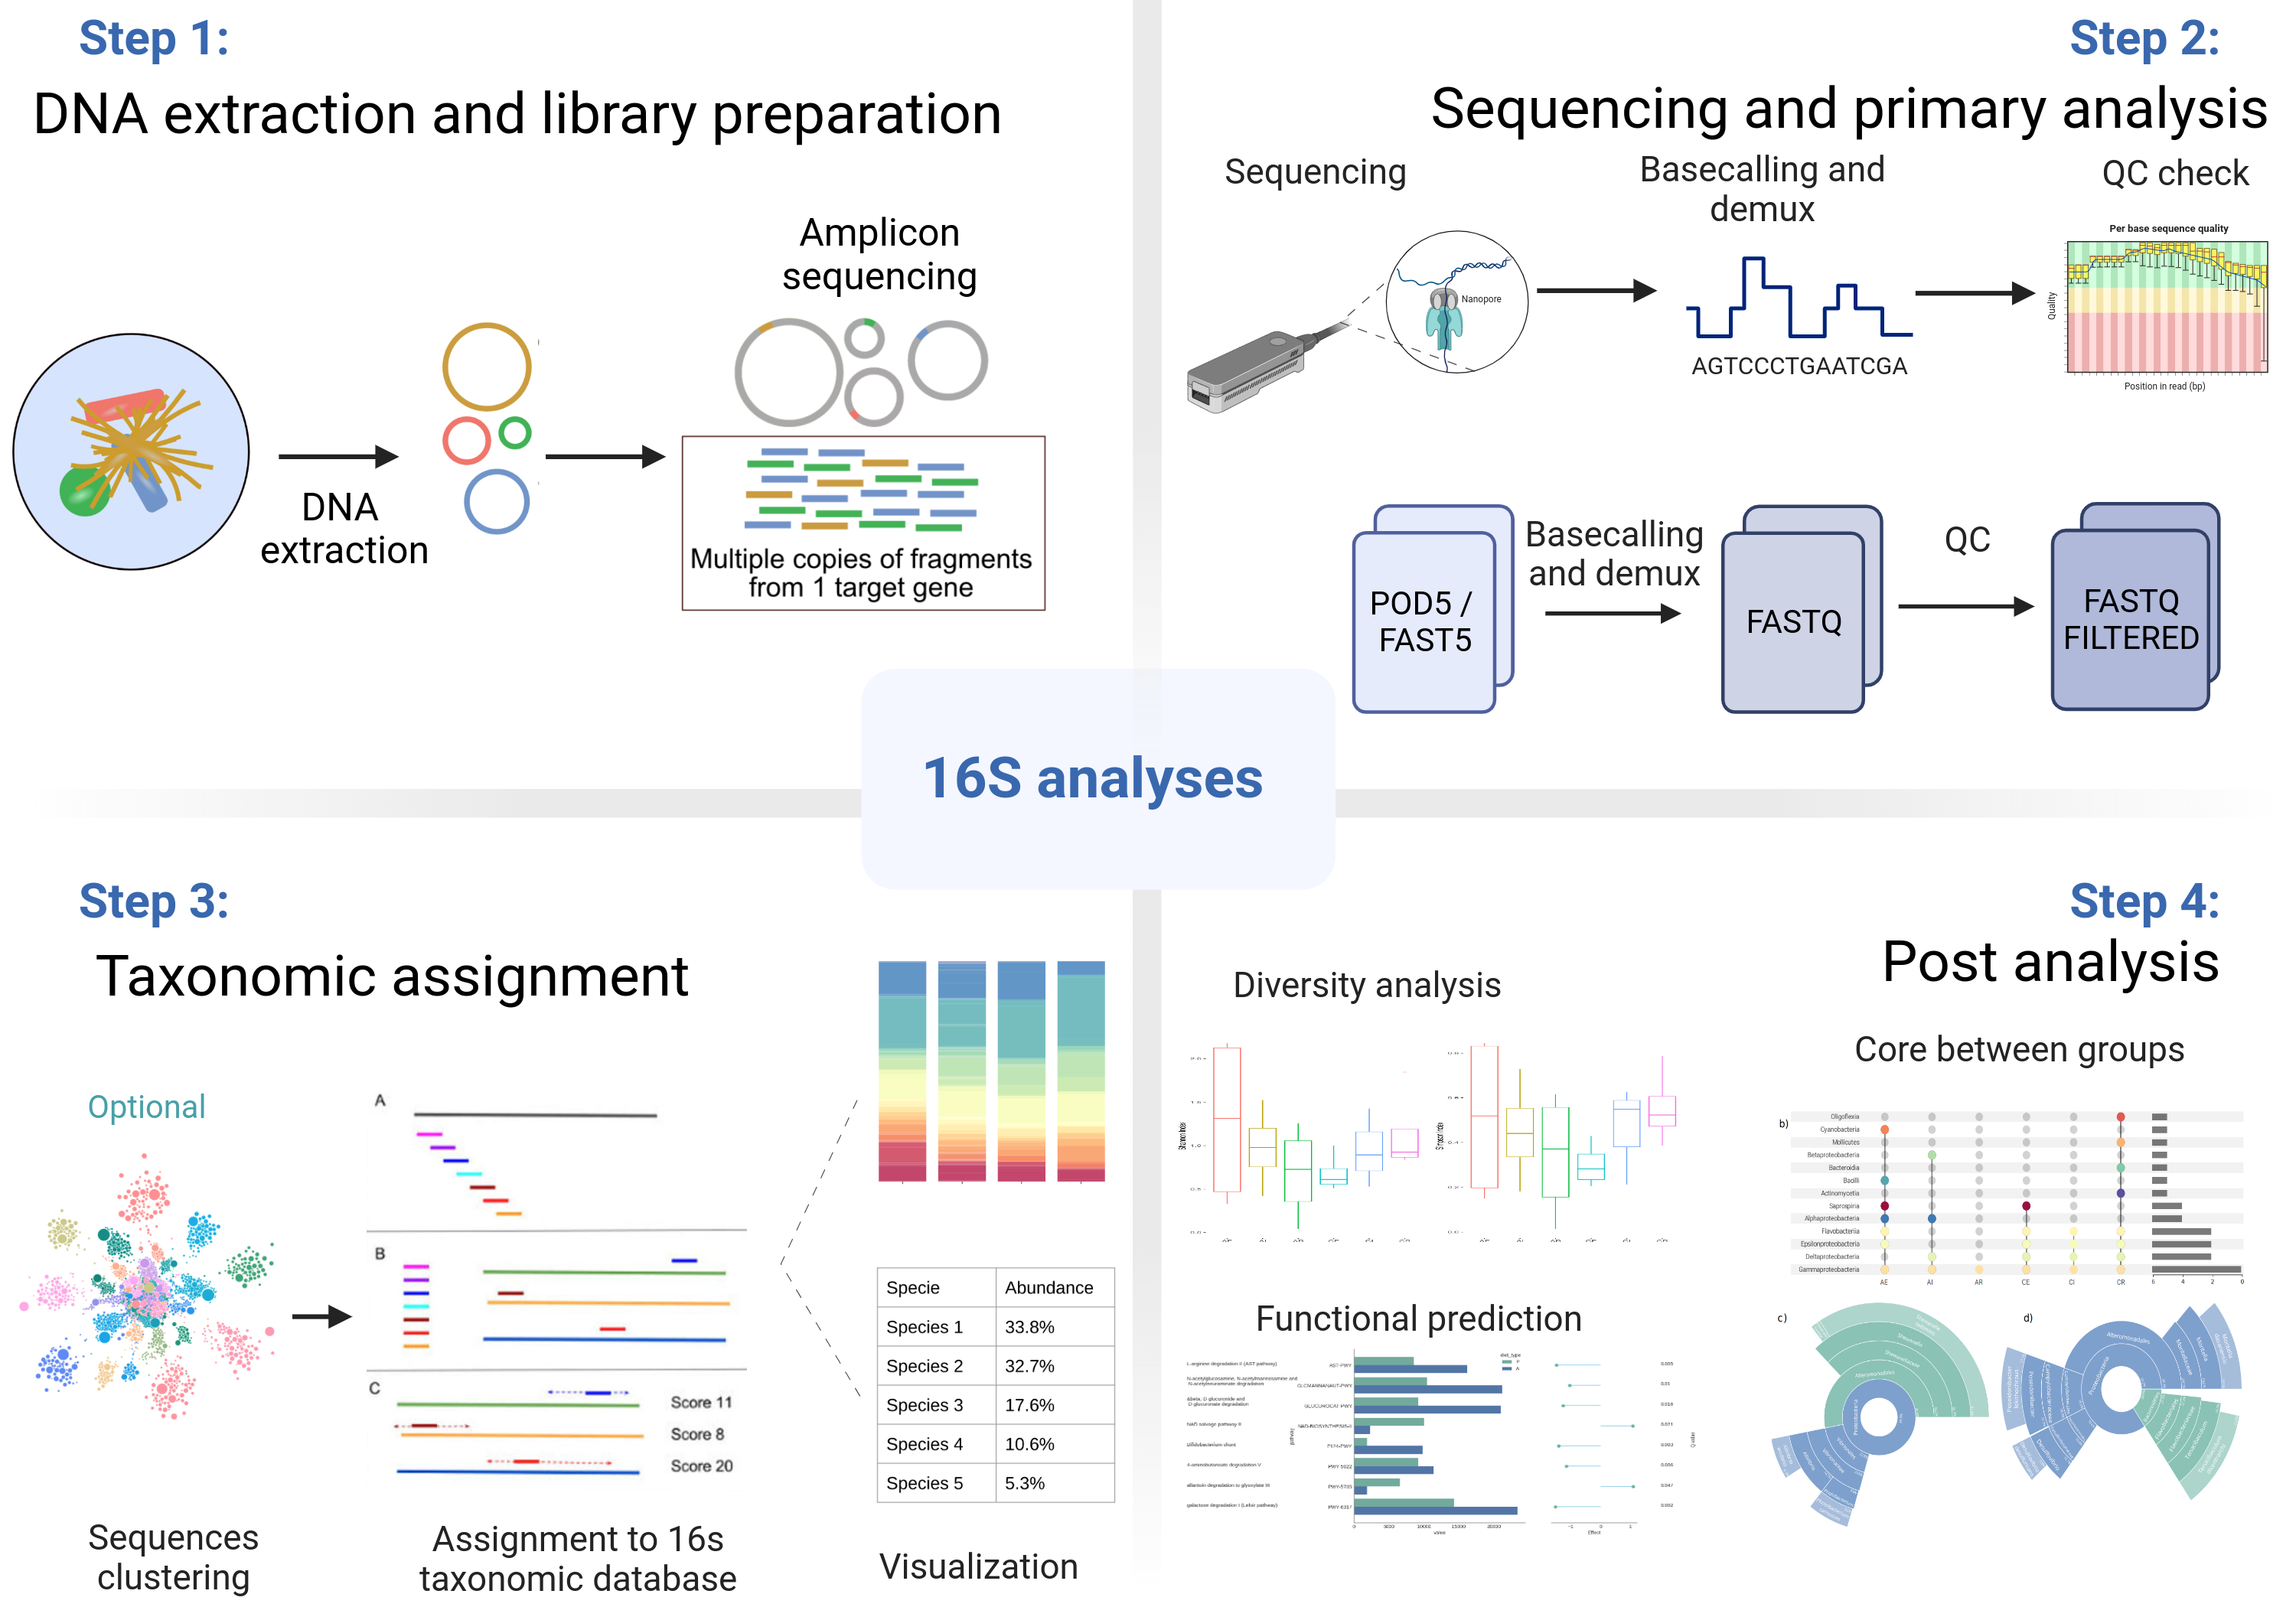
\includegraphics[width=1\linewidth]{images/16s_workflow_schema.jpeg}
%     \caption{Flujo de trabajo estándar para la secuenciación y análisis de secuenciaciones del gen 16S}
%     \label{fig:16S_workflow}
% \end{figure}
\section{Flujo de trabajo}
Se desarrolló un flujo de trabajo automatizado en Nextflow que permite el análisis y la caracterización de secuencias del gen 16S obtenidas mediante dispositivos de secuenciación de Oxford Nanopore. 
El flujo de trabajo está diseñado de manera modular permitiendo que el usuario pueda personalizar su ejecución, agregando o quitando módulos de análisis mediante un archivo de configuración en formato \textit{YAML}.  

El pipeline cuenta con los siguientes módulos: 
\begin{itemize}
    \item Basecalling y demultiplexación (\textit{basecalling}): Este módulo se encarga de realizar el basecalling y demultiplexación de las muestras mediante la herramienta \hl{Guppy}.
    \item Control de calidad (\textit{qc}): Este módulo se encarga de realizar los filtros y control de calidad de las muestras mediante las herramienta Nanoplot y Nanoq.
    \item Asignación taxonómica (\textit{taxonomic\_assignament}): Este módulo se encarga de realizar la asignación taxonómica de las muestras mediante la herramienta BLAST y la base de datos de 16S Genbank. Previo a la asignación taxonómica se realiza un subsampleo de las muestras y un clustering y se convierten los archivos FASTQ a formato FASTA.
    \item Índices de diversidad (\textit{diversity}): Este módulo se encarga de calcular los índices de diversidad de Shannon, Simpson y Chao1 mediante el paquete vegan de R.
    \item Predicción funcional (\textit{functional\_predicction}): Este módulo se encarga de realizar la predicción funcional de las muestras mediante la herramienta PICRUSt2 y la búsqueda de vías metabólicas que presentan diferencias significativas entre grupos mediante la herramienta Lefse.
\end{itemize}

En los módulos de asignación taxonómica, índices de diversidad y predicción funcional mediante scripts en python se resume la información mediante tablas y se generan gráficos de los resultados obtenidos.

En caso de que el flujo de trabajo se esté ejecutando desde la aplicación web, se ejecutará además un módulo extra que permite escribir los resultados en la base de datos.

\subsection{Diseño del flujo de trabajo}
\subsubsection{Bascalling y demultiplexación}
\hl{Me suena más a marco teorico}
Los algoritmos de basecalling desarrollados por Oxford Nanopore Technologies (ONT) permiten determinar la secuencia de nucleótidos a partir de las señales eléctricas generadas por los poros utilizando algoritmos basados en redes neuronales.
Una caracteristica relevante de las redes neuronales es su capacidad de aprender y mejorar sus predicciónes mediante el entrenamiento de la red.
En el caso de los algoritmos de basecalling provistos por Oxford Nanopore sevutilizó un gran volumen de datos de secuenciación de alta calidad y de diferentes organismos incluyendo plantas, animales, bacterias y virus para generar modelos que permitan obtener resultados precisos y confiables\footnote{https://nanoporetech.com/platform/technology/basecalling}.


El entrenamiento de una red neuronal permite obtener módelos que luego se pueden utilizar al ingresar nueevos datos a la red.
En este caso, los algoritmos de basecalling de Oxford Nanopore ofrecen tres modelos diferentes para realizar el bascaling: módelo rapido (FAST), módelo de alta precisión (HAC) y el módelo super preciso (SUP).
El módelo a utilizar durante el basecalling define la configuración utilizada para realizar el basecalling por lo que influye notoramiente en los resultados a obtener, permitiendo utilizar modelos más rápidos y que requieren menos recursos computacionales pero menos precisos, como lo es el modelo fast o modelos mas exhautivos\hl{??} en recursos computacioneles y tiempo requerido pero más precisos, como el modelo SUP.


Actualmente la herramienta Dorado es la herramienta oficial de Oxford Nanopore para realizar el basecalling y la demultiplexación de las muestras, por lo que se utilizará esta herramienta con el modelo SUP para realizar el basecalling y la demultiplexación de las muestras.
\subsubsection{Control de calidad}
Realizar un correcto control de calidad  de las secuencias es un paso fundamental en cualquier análisis bioinformático, esto permite eliminar secuencias de baja calidad, eliminando posibles sesgos producidos por el porcentaje de error permitiendonos obtener resultados más precisos


La calidad de una base se representa mediante puntajes de calidad denomiandos \textit{q-score}, los cuales se pueden calular mediante la siguiente formula:
\begin{equation}
    Q = -10 \log_{10}(P)
    % Q = -10log10(e)
\end{equation}
Al realizar filtros o control de calidad se suele resumir la calidad de la secuencia mediante un número que representa la calidad promedio de la secuencia a lo largo de todas las bases. 

Herramientas clásicas como  FastQC y Fastp primero promedian los puntajes de calidad de cada base y luego aplican la formula de calidad sobre el valor obtenido, lo que puede llevar a errores en el cálculo de la calidad de las secuencias cuando los valores de qscore varian mucho a lo largo de la secuencia como en el caso de secuenciaciones de Oxford Nanopore.
En el caso de tecnologías de lecturas cortas como Illumina donde la calidad no varia mucho a lo largo de la secuencia, este método es aceptable, pero en el caso de secuenciaciones de Oxford Nanopore donde la calidad varia mucho a lo largo de la secuencia, este método puede llevar a obtener valores de calidad más altos de los que realmente son.

Es por esto que se decidió utilizar NanoPlot para el control de calidad y Nanoq para los filtros de calidad ya que el cálculo de calidad es más adecuado para la tecnología de secuenciación que se esta utilizando.%calculan la probabilidad de error por cada base y luego promedian los valores obtenidos, lo que permite obtener resultados más precisos y confiables en el cálculo de la calidad de las secuencias con Oxford Nanopore.
% NanoPlot y Nanoq a diferencia de herramientas ampliamente utilizadas en bioinformática como Fastp y FastQC, estan pensadas para ser utilizadas con datos de secuenciación de Oxford Nanopore, teniendo en consideración algunas caracteristicas relevantes a la hora de procesar lecturas largas como lo es la variabilidad en los puntajes de calidad a lo largo de la secuencia.
% NanoPlot y Nanoq calculan la probabilidad de error por cada base y luego promedian los valores obtenidos, lo que permite obtener resultados más precisos y confiables en el cálculo de la calidad de las secuencias con Oxford Nanopore.


%ya que calculan el error de la secuencia primero promediando los puntajes de calidad de cada base y luego aplicando la formula de calidad sobre el valor obtenido, lo que puede llevar a errores en el cálculo de la calidad de la secuencia cuando los valores de qscore varian mucho a lo largo de la secuencia como en el caso de secuenciaciones de Oxford Nanopore.
%Existen diferentes herramientas como Fastp y FastQC que utilizan la primera metodología para el cálculo de calidad, mientras que herramientas como  Nanoplot y Nanoq utiliza la segunda metodología. 
%Se decidió utilizar NanoPlot y Nanoq para realizar el control y filtros de calidad de las secuencias debido a que calculan la probabilidad de error por cada base y luego promedian los valores obtenidos, lo que permite obtener resultados más precisos y confiables en el cálculo de la calidad de las secuencias.


Para los filtros de calidad se dicidió utilizar una calidad promedio de \hl{15-16} lo que implica una precisión del \hl{96.8-97.4\%}




% y en filtros de calidad (Fastp y Nanoq) para determinar cuál de ellas se ajusta mejor a las necesidades del análisis de secuencias de Oxford Nanopore.








% La mayoría de las herramientas bioinformáticas desarrolladas para esta tarea utilizan alguna de las siguientes metodologías:
% \begin{itemize}
%     \item Cálculo de calidad en base a un promedio de los puntajes de calidad: Se promedían los puntajes de calidad de cada base y luego se calcula el puntaje de calidad y probabilidad de error de la secuencia aplicando el logaritmo de la formula de calidad.
%     \item Cálculo de calidad utilizando una conversión previa de los puntajes de calidad a probabilidades: Los puntajes de calidad de cada base se convierten primero a probabilidad de error mediante la formula de calidad y luego se promedian los porcenajes de error  obtenidos y se calcula el puntaje de calidad de la secuencia.
% \end{itemize}

% ----------------

Para reducir los costos computacionales en el paso de asignación taxónomica se decidió hacer un subsampling de las muestras con un valor por defecto de 100.000 lecturas. 
Como se sabe que la calidad de las lecturas es un factor importante en la asignación taxonómica e influye directamente en la precisión de la asignación, se decidió realizar este muestro seleccionando las mejores lecturas en base a la calidad obtenida, para ello se utilizó la herramienta Filtlong.

Este muestreo no es aleatorio, es basado en la calidad de las lecturas utilizando la herramienta filtlong. 
Por defecto Filtlong realiza esta selección de las mejores lecturas ponderando de igual manera la calidad y la longitud de las lecturas, en este caso, considerando que se secuenció el amplicon completo del gen 16S y que se realizó un filtro previo para eliminar lecturas que no se encuentren en el rango deseado (entre 1000 y 2000 pares de bases), se decidió realizar el filtro de las lecturas ponderando la calidad de las lecturas con un valor de 10 y el largo de las lecturas con un valor de \hl{0}. 


\begin{itemize}
    \item Nanoq y nanoplot calculan la calidad de la manera correcta , fastq y faspt no
    \item se filtro por una calidad de 15 lo que es un 96.8\% de precisión
    \item entre 1000 a 2000
    \item filtros se hicieron en base a las mejores secuencias (mejor = calidad)
\end{itemize}
\subsubsection{Asignación taxonomica}
Para la asignación taxonómica se decidió utilizar Blast junto con la base de datos de 16S de Genbank, 

\begin{itemize}
    \item pq un clustering al 95\% de identidad
    \item tiempos de ejecucion blast solo, mmseqs + blast rep, emu, minimap2 (nanopre), krekaaen
    \item similitud de resultados entre las diferentes herramientas
    \item porque el valor del  subsampling (debería hacer experimentos con diferentes valores?)

\end{itemize}
Para realizar la asignación taxonómica se propone realizar un clustering utilizar la herramienta BLAST con la base de datos de 16S de Genbank.
clusterng con diferentes calidades y porcentajes de identidad \hl{boxplot de cantidad de especies que se pierden o grafico de puntos de cantidad de especies detectadas vs en el eje x el valor del subsampling (tal vez un jitter)}



\hl{emu / kraken / minimap / blast / blast con clustering}

%% comparacion con emu https://www.nature.com/articles/s41592-022-01520-4
----------------- o -----------------
\hl{explicar que el clustering elige una secuencia representativa}

Se evalúo el impacto de la calidad de las muestras al realizar el clustering evaluando la cantidad de clusters generados, cantidad de cluster con menos de 10 secuencias (0.01\% de las secuencias) y el porcentaje de identidad de las secuencias del cluster con la secuencia representativa del cluster.


Para esto se realizó el clustering de las muestras con diferentes valores de calidad (Q10-Q12-Q14-Q16-Q18) y un porcentaje de identidad de \hl{XX}, se observó que al aumentar la calidad de las muestras se reducía la cantidad de clusters generados, \hl{lo que indica que las muestras de baja calidad generan clusters con mayor cantidad de secuencias, lo que puede llevar a una asignación taxonómica incorrecta.-- hablar del porcentaje de identidad entre cluster}

%, el porcentaje de secuencias que se asignan en un primer hit. En caso de las secuencias que no el primer hit no corresponde al mismo hit que


\subsubsubsection{Comparación de herramientas de asignación taxonómica}
Apart from the misclassification of the XXX reads, the Nanopore results were close to the composition of the mock community 

clustering sea version alternativa / experimental



Para definir el número de lecturas óptimo para realizar el muestreo aleatorio se comparaon los resultados a nivel de especie utilizando valores desde 10.000 a 100.000 lecturas en un rago de 10.000 en 10.000. 
Para el experimento se utilizo una calidad de 15 y clustering con un valor de 95\% de identidad.
Los resultados se presentan en la figura:
\subsubsection{Caracterización de grupos}
The functional inference of microbiota was investigated based on PICRUSt2 software.

The polished representative sequence of clusters derived from NanoCLUST was used for functional inference analysis using PICRUSt270. 
The abundance of predicted pathways based on MetaCyc annotation


El índice de Chao1 permite estimar la riqueza de especies en una muestra, es decir el número total de especies. A diferencia del índice de Chao2 el cual requiere información de presencia o ausencia de un taxon el índice de Chao1 utiliza los valores de abundancias de cada especie para la estimación.
Se decidió incluir este índice por su  por su capacidad para estimar la riqueza de especies de manera precisa, incluso en muestras incompletas o donde hay un alto numero de especies raras\hl{citas}
 mientras que los índices de Shannon y Simpson permiten estimar la diversidad de especies en una muestra.


Dentro de las diferentes herramientas que se pueden utilizar para la prediccón funcional se encuentra PICRUSt2, Tax4Fun,  PanFp
. 
For example, LEfSe5 is a popular method for identifying differentially abundant taxa that first converts read counts to percentages. Accordingly, read count tables are often rarefied before being input into this tool so that variation in sample read depth does not bias analyses. Without addressing the variation in depth across samples by some approach, the richness can drastically differ between samples due to read depth alone.


The rarefied feature table was first converted into LEfSe format using the LEfSe script format_input.py5. We then ran LEfSe on the formatted table using the run_lefse.py script with default settings and no subclass specifications. Briefly, this command first normalized the data using total sum scaling, which divides each feature count by the total library size. Then it performed a Kruskal-Wallis (which in our two-group case reduces to the Wilcoxon rank-sum) hypothesis test to identify potential differentially abundant features, followed by linear discriminant analysis (LDA) of class labels on abundances to estimate the effect sizes for significant features. From these, only those features with scaled LDA analysis scores above the threshold score of 2.0 (default) were called as differentially abundant. This key step is what distinguished LEfSe from the Wilcoxon test approach based on relative abundances that we also ran. In addition, no multiple-test correction was performed on the raw LEfSe output as only the p-values of significant features above-threshold LDA scores are returned by this tool.
%https://www.nature.com/articles/s41467-022-28034-z

lefse 1Millones (galaxy) 
%http://galaxy.biobakery.org
leer hilo de google %https://groups.google.com/g/lefse-users/c/zGPzu9o3ct8
\subsection{Archivo de configuración} \label{subsection:conf_file}
El formato YAML se caracteriza por ser un formato de serialización de datos legible por humanos y fácil de interpretar por máquinas.
Tiene una estructura jerárquica que permite la representación de datos de manera más clara y concisa que otros formatos como JSON o XML.

Mediante este archivo de configuración se van a especificar los parámetros necesarios para la ejecución del flujo de trabajo.
Además, el archivo de configuración incluye información sobre los archivos de entrada del flujo de trabajo, nombres de las muestras y grupos asociados.

Para especificar parámetros de un módulo se debe indicar la clave asociada del módulo seguido por \textit{:} y a continuación el nombre del parámetro a modificar y su valor en formato \textit{clave: valor} (muestra: grupo) en la siguiente línea.

Las claves utilizadas en el archivo de configuración para los módulos son las siguientes: \textit{basecalling}, \textit{qc}, \textit{taxonomic\_assignament}, \textit{diversity} y \textit{functional\_prediction}.
A continuación se detallan los parámetros que se pueden modificar en el archivo de configuración y se presenta un ejemplo de archivo de configuración.%(\ref{verb:config}):

\begin{itemize}
    \item \textit{run}: Permite activar o desactivar el módulo. Los valores posibles son ``ON'' o ``OFF''. 
    \item \textit{qc.min\_length}: Permite modificar la longitud mínima requerida de las secuencias. Por defecto es 1000.
    \item \textit{qc.max\_length}: Permite modificar la longitud máxima permitida de las secuencias. Por defecto es 2000.
    \item \textit{qc.min\_qscore}: Permite modificar la calidad mínima requerida de las secuencias. Por defecto es 15 (96,8\% de precisión) .
    \item \textit{qc.subsampling}: Permite modificar la cantidad de lecturas utilizadas para el subsampleo. Por defecto es 100.000.
    \item \textit{qc.save\_reads}: Permite activar o desactivar el guardado de los archivo fastq filtrados en el directorio de resultados. Valores posibles True o False. Por defecto False. 
    \item \textit{taxonomic\_assignament.perc\_identity}: Porcentaje de posiciones idénticas en la secuencia de alineamiento.
    \item \textit{taxonomic\_assignament.evalue}: Valor máximo de evalue aceptado.
    \item \textit{taxonomic\_assignament.qcovs}: Porcentaje de cobertura mínima de alineamientos con altos puntajes.
    \item \textit{taxonomic\_assignament.blast\_db}: Permite ingresar la ruta al directorio que contiene la base de datos de 16S de Genbank (ver sección~\ref{pipeline:how_to_run} para más información).
    \item \textit{group}: Permite ingresar los grupos asociados a las muestras en formato \textit{clave:valor}.
    \item \textit{input}: Permite ingresar el archivo en formato CSV que contiene las columnas samples y fastq.
    \item \textit{outdir}: Permite ingresar el directorio donde se guardaran los resultados del flujo de trabajo.
    \item \textit{samples}: Archivo en formato csv que permite especificar  el nombre de las muestras y su ubicación en el sistema de archivos.
\end{itemize}

A continuación se presenta un ejemplo de archivo de configuración donde el módulo de basecalling se encuentra desactivado, y los módulos de control de calidad, asignación taxonómica, índices de diversidad y predicción funcional se encuentran activados.
Además se especifican todos los parámetros por defecto del flujo de trabajo, junto con un ejemplo de grupos asociados a las muestras y la ruta al archivo de metadata.



% Además se requiere un archivo de configuración en formato YAML que contenga los parámetros necesarios para la ejecución del pipeline. 
% A continuación se presenta un ejemplo de archivo de configuración:

\begin{verbatim}
  basecalling:
    run: 'OFF'
    save_reads: False
  qc:
    max_length: '2000'
    min_length: '1000'
    min_qscore: '15'
    run: 'ON'
    subsampling: '50000'
    save_reads: False
  taxonomic_assignament:
    run: 'ON'
    blast_db: 'db/'
  diversity:
    run: 'ON'
  functional_prediction:
    run: 'ON'
  group:
    K1.1: Control K
    L1.1: Control L
    L1.2: Control L
    P1.1: No impactadas
    P1.2: No impactadas
    P7.2: Impactadas
    P8.1: Impactadas
  input: samples.csv
  outdir: results
\end{verbatim}
\label{verb:config}

\textit{samples.csv} es un archivo de texto separado por comas (formato CSV) que contiene la información de las muestras a analizar mediante las columnas \textit{samples} y \textit{fastq}. 
La columna samples debe contener el nombre con el que se quiere identificar a las muestras y la columna \textit{fastq} la ruta al archivo de secuenciación en formato \textit{fastq}.

\subsection{Estructura del flujo de trabajo}
%El flujo de trabajo se encuentra estructurado por módulos, donde cada módulo se encarga de realizar una tarea específica.

\subsubsection{Basecalling y demultiplexación}
La entrada de este módulo son archivos en formato \textit{POD5} que contienen la información secuenciada.
El basecalling y demultiplexación se realizan mediante la herramienta Guppy.
%Por defecto se realizará el basecalling de alta preción (HAC).

Para ejecutar este módulo el usuario deben ingresar los siguientes parámetros en el archivo de configuración:
\begin{itemize}
    \item \textit{pod5\_dir}: Directorio que contiene los archivos de secuenciación en formato POD5.
    \item \textit{guppy\_basecalling\_config}: Archivo de configuración a utilizar para hacer el basecalling.
    \item \textit{guppy\_barcoding\_kits}: Kit de barcoding a utilizar para hacer la demultiplexación.
    \item \textit{save\_reads}: Permite activar o desactivar el guardado de los archivos demultiplexados. Valores posibles True o False. Por defecto False.
\end{itemize} 

Por defecto este módulo entrega un archivo HTML con el reporte de la demultiplexación y el basecalling de las muestras (generado con MultiQC), el cual se almacena en la carpeta QC/multiqc\_guppy.html.
En caso de que el usuario quiera almacenar los archivos demultiplexados, debe activar la opción \textit{basecalling.save\_reads} en el archivo de configuración.


\subsubsection{Control de calidad}
Este módulo siempre se ejecuta y es el encargado de realizar los filtros y control de calidad de las muestras.
La entrada de este módulo son archivos en formato \textit{Fastq}, que pueden ser provenientes del módulo anterior (\textit{basecalling y demultiplexación}) o pueden ser indicados por el usuario a través del archivo de configuración.
El control de calidad se realiza mediante la herramienta NanoPlot (antes y después de los filtros).
Los filtros de calidad son llevados a cabo con la herramienta Fastp, utilizando los siguientes parámetros:
\begin{itemize}
    \item calidad mínima: por defecto 15 o valor ingresado en el archivo de configuración \textit{qc.min\_qscore} (\textit{-q 15})
    \item \textit{--cut\_mean\_quality 15}: Permite eliminar bases de baja calidad en los extremos de la secuencia, por defecto 15 (uso en conjunto con \textit{--cut\_front}, \textit{--cut\_tail})
    \item longitud mínima requerida: por defecto 1000 o valor ingresado en el archivo de configuración \textit{qc.min\_length} (\textit{--length\_required 1000}) 
    \item longitud máxima permitida: por defecto 2000 o valor ingresado en el archivo de configuración \textit{qc.max\_length} (\textit{--length\_limit 2000})
    \item deshabilitar la eliminación de adaptadores (\textit{--disable\_adapter\_trimming}) (no modificable)
    \item deshabilitar la eliminación de colas poly g (\textit{--disable\_trim\_poly\_g}) (no modificable)
\end{itemize}

Además, este módulo cuenta con un script desarrollado en Python que permite graficar la longitud promedio versus la calidad promedio de las muestras después de los filtros.

El output de este módulo es una carpeta llamada \textit{QC} que contiene los siguientes directorios:
\begin{itemize}
    \item \textit{fastq\_filtered}: Directorio con archivos FASTQ de las secuencias filtradas (obtenidas con fastp).
    \item \textit{fastp\_reports}: Directorio con los reportes de los filtros de calidad en formato JSON y HTML (obtenidos con fastp).
    \item \textit{nanoplot\_reports/raw|filtered}: Directorio con los reportes de control de calidad de las muestras antes y después de los filtros (obtenidos con NanoPlot).
    \item \textit{multiqc}: Reporte en formato HTML con el resumen de los reportes de NanoPlot y Fastp para los archivos antes y después de los filtros de calidad.
    \item \textit{quality\_plot.pdf}: Gráfico de la longitud promedio versus la calidad promedio de las muestras después de los filtros en una ventana de las posiciones de 1400 a 1600 pares de bases.
\end{itemize}

A continuación se presenta un ejemplo del gráfico de calidad y longitud promedio de las muestras generado por el pipeline (Figura~\ref{fig:pipeline-quality-plot}).
\begin{figure}[H]
    \centering
    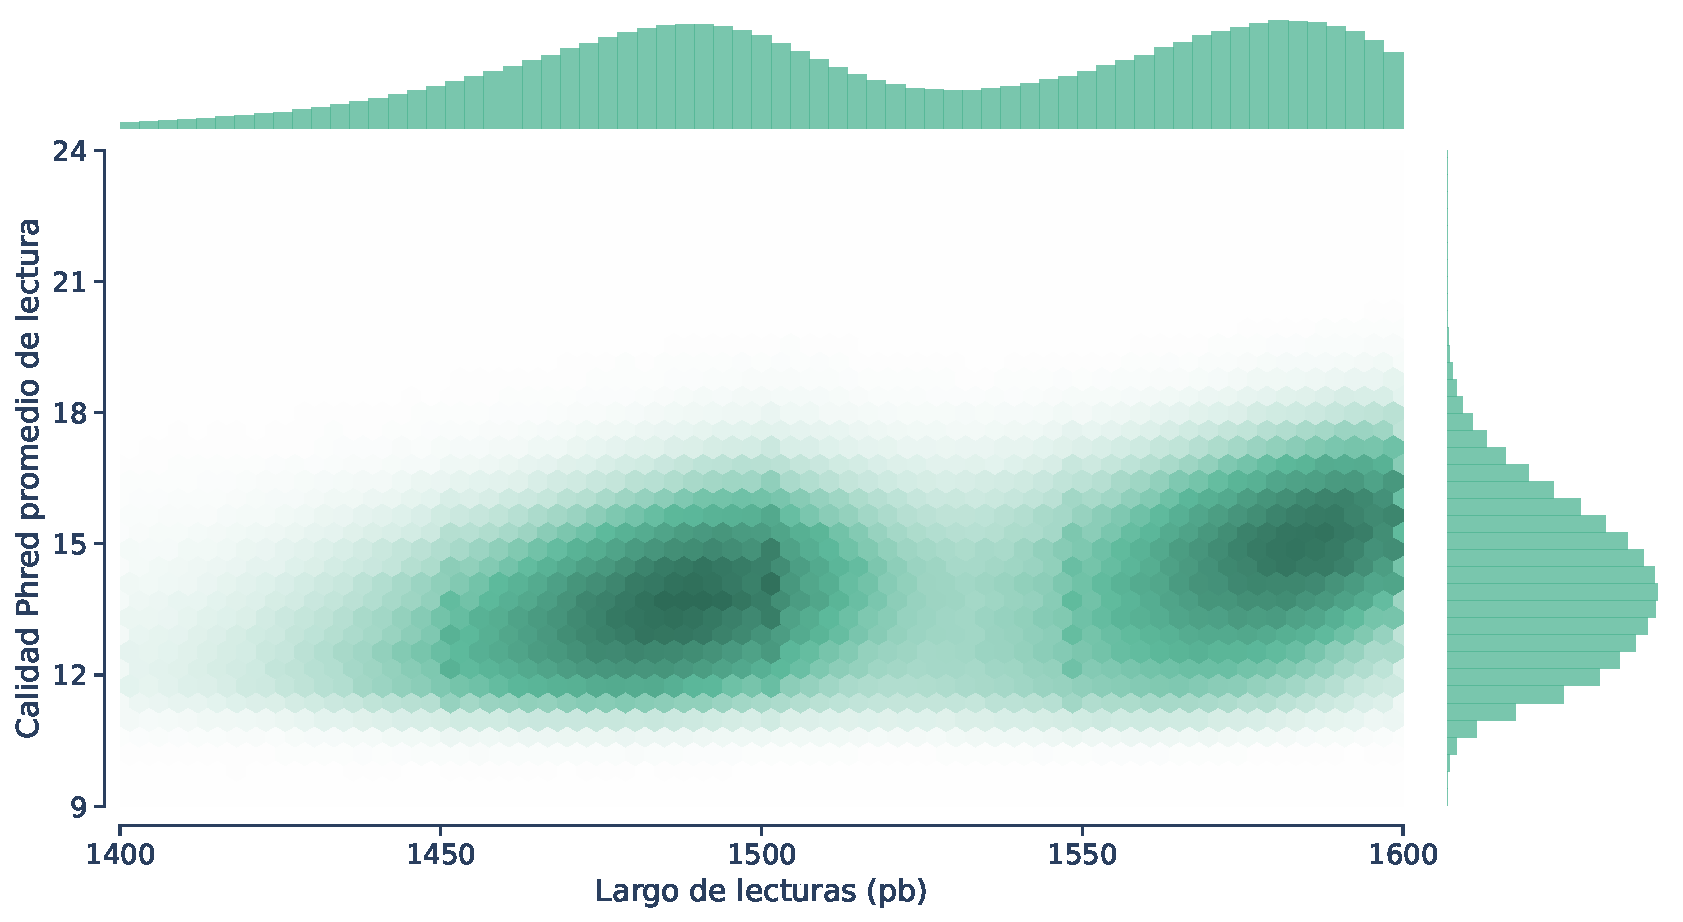
\includegraphics[width=0.85\linewidth]{images/pipeline/quality_plot.pdf}
    \caption{Gráfico de calidad vs longitud promedio. En el eje X esta la longitud de las lecturas, mientras en el eje Y se encuentra la calidad promedio.}
    \label{fig:pipeline-quality-plot}
\end{figure}
\subsubsection{Asignación taxonómica}
Este módulo se ejecuta siempre que el parámetro de asignación taxonómica sea ``ON'' en el archivo de configuración. 
La ruta a la base de datos debe ser especificada mediante el parámetro \textit{taxonomic\_assignament.blast\_db}.
La entrada de este módulo son archivos en formato \textit{FASTQ} que provienen del módulo anterior (\textit{control de calidad}).

Previo a la asignación taxonómica, se realiza un subsampleo de las muestras con la herramienta SeqKit para evitar sesgos en la caracterización de la comunidad microbiana debido a alguna desproporción en la cantidad de lecturas de las muestras.
La cantidad de lecturas utilizadas para el subsampling por defecto es 100.000 o el valor ingresado por el usuario en el archivo de configuración \textit{qc.subsampling}.
Posterior a ello se convierten los archivos FASTQ a formato FASTA mediante la herramienta SeqKit.

La asignación taxonómica se realiza mediante la herramienta BLAST (algoritmo blastn) con la base de datos de 16S de Genbank. 
\hl{Para aceptar un match con la base de datos se requiere un valor de identidad mayor al 97\%, una cobertura mayor al 85\% y un evalue menor a 1e-6.}
\hl{Se eliminan todas las taxas con menos de 0.01\% de abundancia.}

Posterior a la asignación taxonómica, mediante la herramienta TaxonKit se obtiene el linaje completo de todas las especies asignadas con BLAST, este resultado se formatea mediante la herramienta CSVTk. 
Esto se realiza con el objetivo de poder graficar todas las categorías taxonómicas tanto en los gráficos de barras apiladas como en el gráfico circular jerárquico.

Mediante un script en python se realiza un resumen de la asignación taxonómica obtenida con BLAST de todas las muestras y los linajes asociados a cada especie en un solo archivo. Además, se generan archivos por cantidad de lecturas y porcentaje, por cada categoría taxonómica y por muestra y grupo (en caso de ingresarse en el archivo de configuración).
Estos archivos son utilizados como entradas para los scripts que generan los gráficos de barras apiladas y  el gráfico circular jerárquico.


En el caso del gráfico circular, se buscan todas las taxonomías compartidas entre las muestras que tengan una abundance mayor al 1\% en al menos una muestra. 
Una vez que se identifican, se suman las lecturas asignadas a cada taxonomía en todas las muestra del grupo y se grafica el porcentaje de lecturas asignadas a cada taxonomía en todas las muestras del grupo como un valor único.



El output de este módulo es una carpeta llamada \textit{taxonomic\_assignament} que contiene los siguientes directorios:
\begin{itemize}
% \item \hl{blast\_out}
\item plots: Este directorio contiene los siguientes directorios:
\begin{itemize}
    \item taxonomy\_plots: Directorio con los gráficos de barras apiladas de las taxonomías. Contiene cuatro tipos de gráficos: 
    \begin{itemize}
        \item barras apiladas por muestra utilizando el valor porcentual.
        \item barras apiladas por muestra utilizando la cantidad de lecturas.
        \item barras apiladas por grupos utilizando el valor porcentual.
        \item barras apiladas por grupos utilizando la cantidad de lecturas.
    \end{itemize}
    \item core\_plot: Directorio con los gráficos circulares jerárquicos de las taxonomías compartidas entre las muestras. Habrá un gráfico general que busca las similitudes en todas las muestras, y un gráfico por cada grupo ingresado (en caso de ingresar grupos)(Figura~\ref{fig:pipeline-core}).
\end{itemize}
 \end{itemize}
A continuación se presentan ejemplos de los gráficos generados en este módulo. La figura~\ref{fig:pipeline-stacked-sample} presenta un gráfico de barras apiladas por muestra utilizando el valor porcentual y la categoría de clase, mientras que la figura~\ref{fig:pipeline-stacked-group} muestra un gráfico de barras apiladas por grupos utilizando el valor porcentual.
\begin{figure}[H]
    \centering
    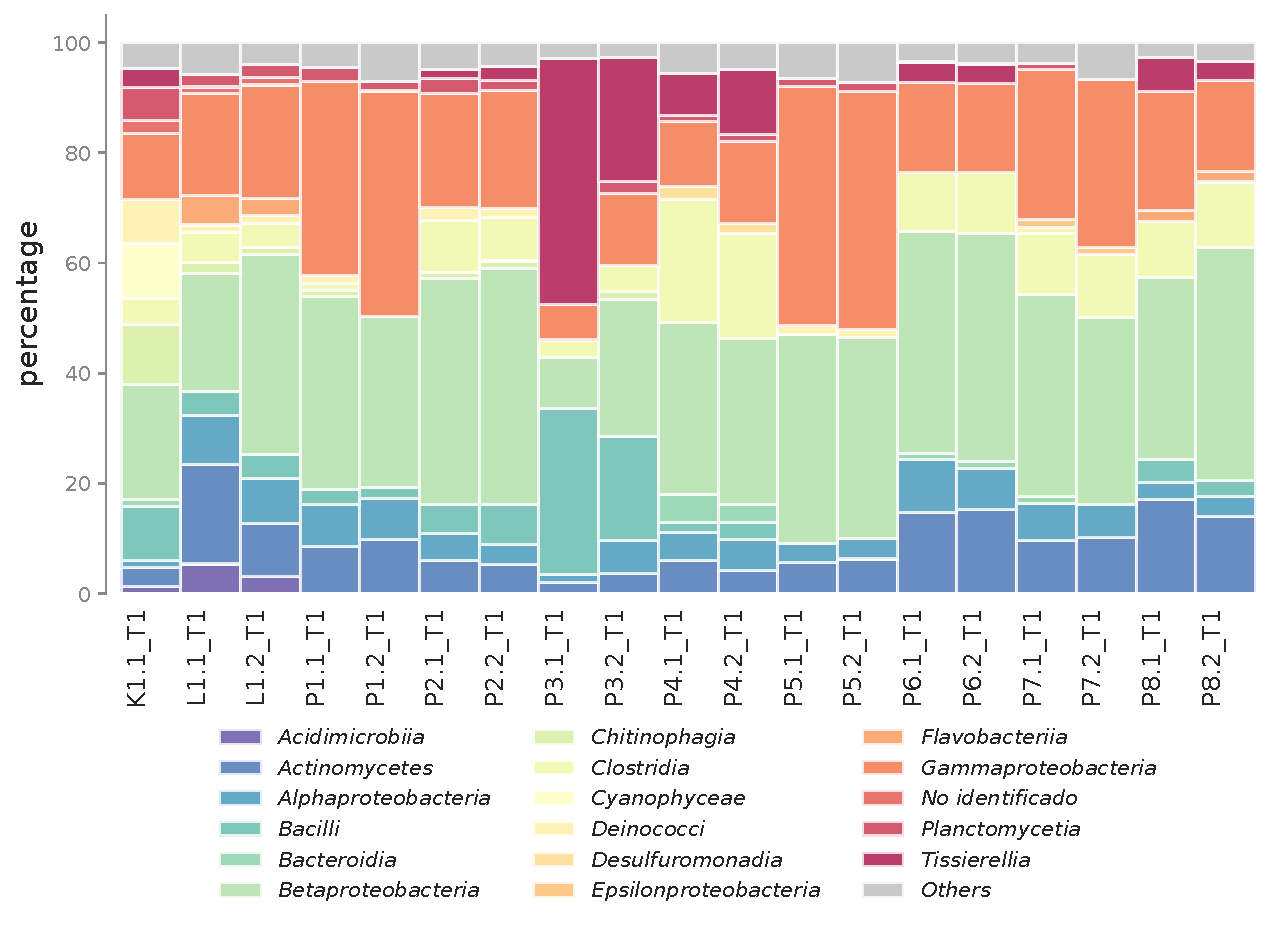
\includegraphics[width=1\linewidth,height=0.4\textheight]{images/pipeline/class_samples_percentage.pdf}
    \caption{Gráfico de barras apiladas por muestra utilizando el valor porcentual y la categoría de clase}
    \label{fig:pipeline-stacked-sample}
\end{figure}
\begin{figure}[H]
    \centering
    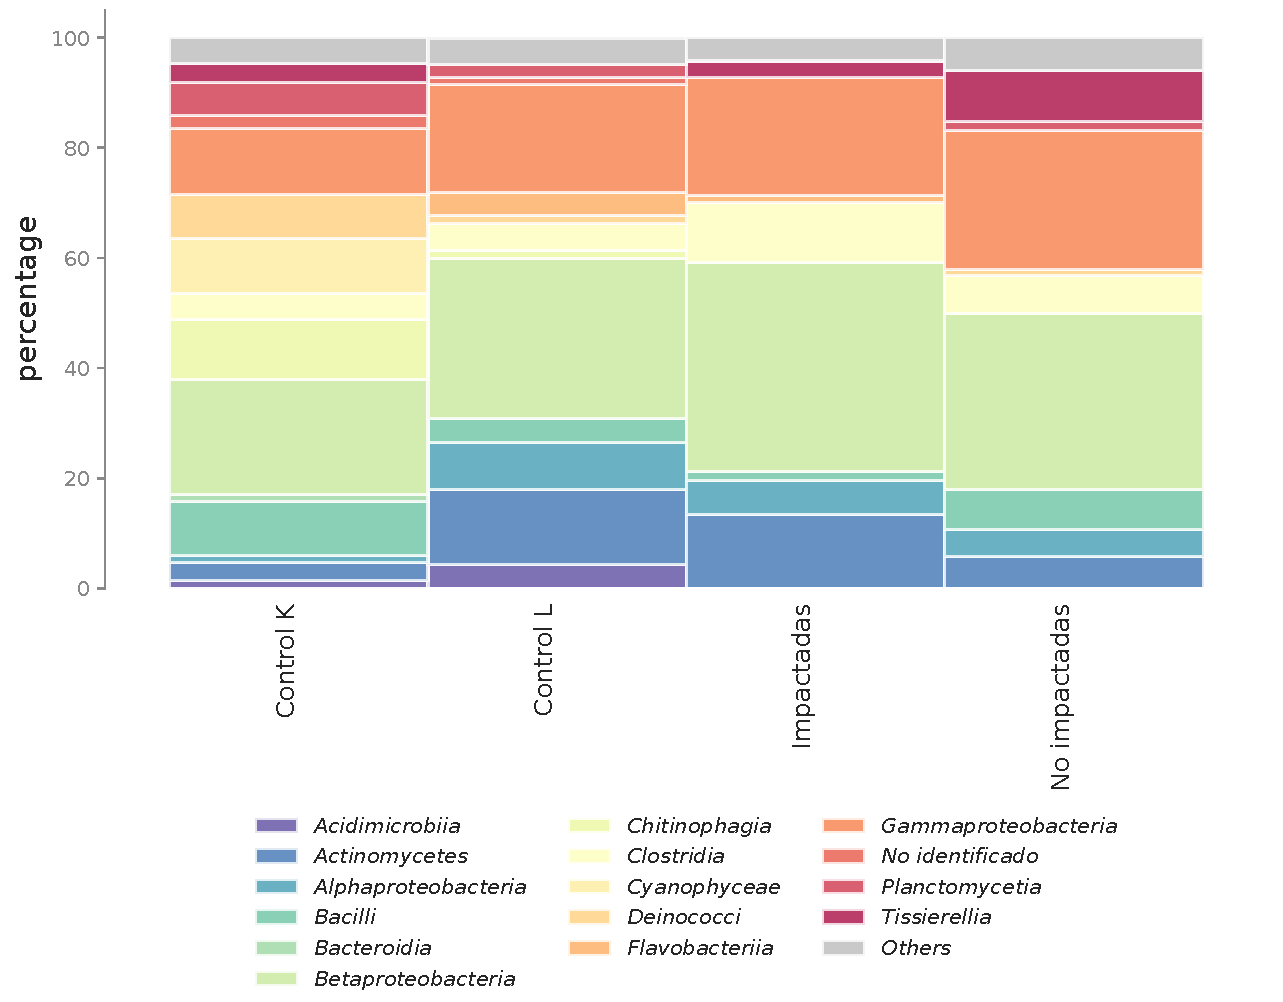
\includegraphics[width=1\linewidth,height=0.4\textheight]{images/pipeline/class_grouped_percentage.pdf}
    \caption{Gráfico de barras apiladas por grupos utilizando el valor porcentual y la categoría de clase}
    \label{fig:pipeline-stacked-group}
\end{figure}

La figura~\ref{fig:pipeline-core} presenta un gráfico circular jerárquico generado para el grupo de muestras categorizadas como No impactadas.
Este gráfico muestra todas las taxonomías compartidas entre las muestras del grupo No impactadas.
\begin{figure}[H]
    \centering
    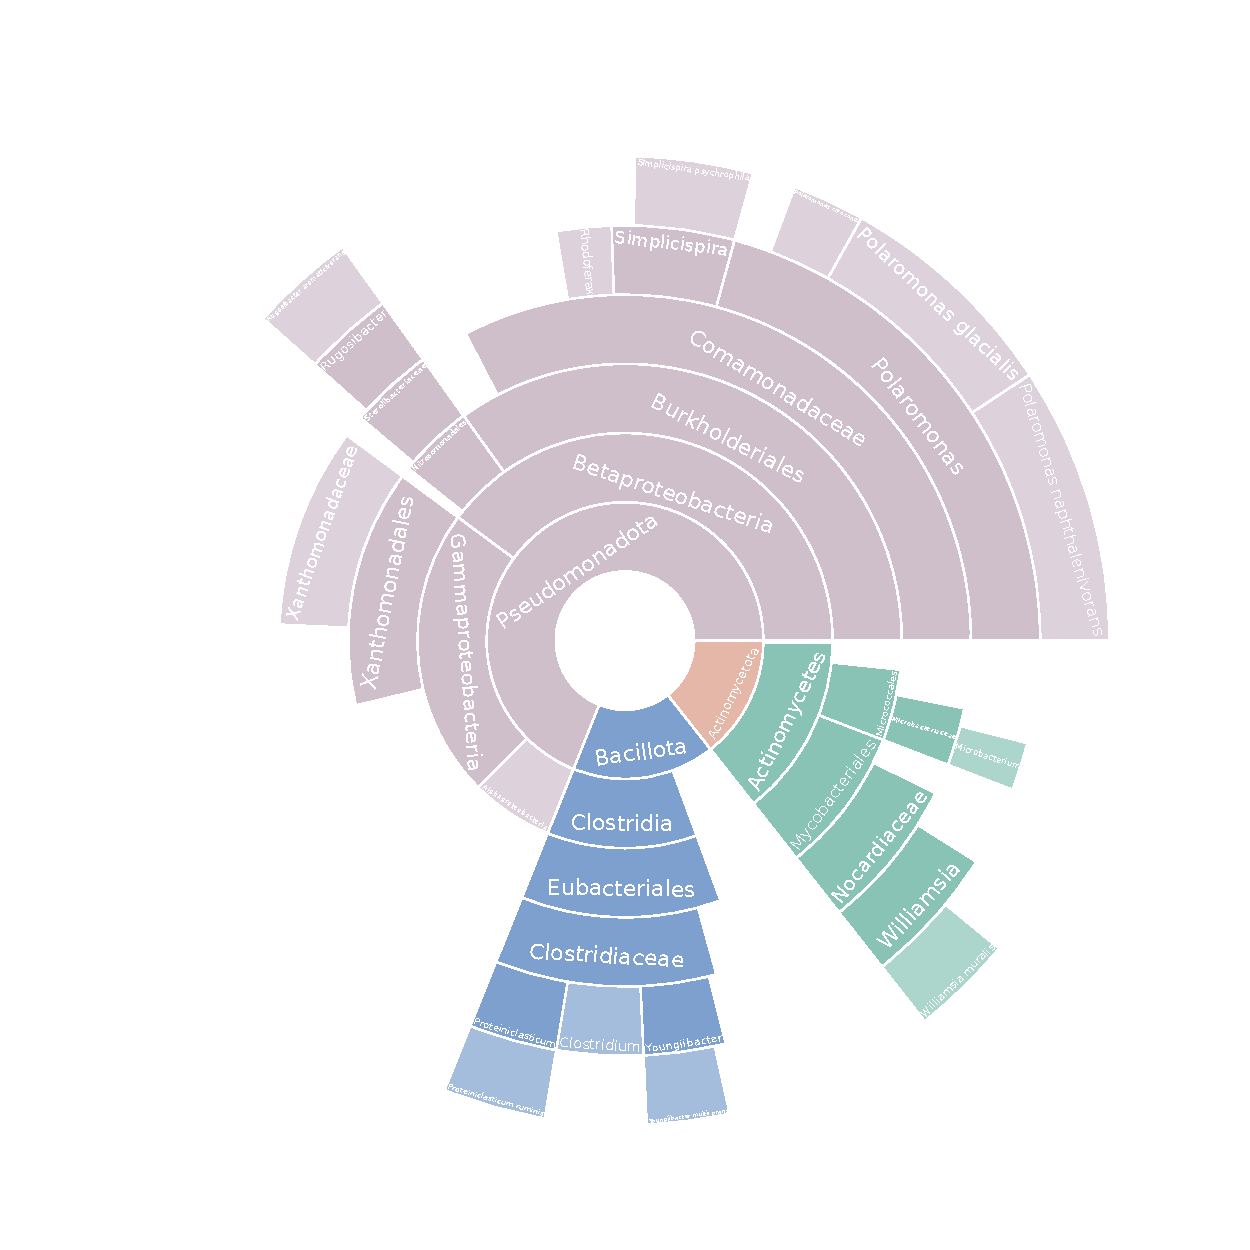
\includegraphics[width=0.9\linewidth]{images/pipeline/core_Impactadas.pdf}
    \caption{Gráfico jerárquico generado para el grupo de muestras categorizadas como No impactadas}
    \label{fig:pipeline-core}
\end{figure}

\subsubsection{Indices de diversidad}
Este módulo solo se ejecutara si el parámetro \textit{diversity.run} es ``ON'' en el archivo de configuración. 
Para poder ejecutarlo se requiere que el usuario haya ingresado grupos asociados a las muestras en el archivo de metadata.

El cálculo de los índices de diversidad se realizará utilizando el paquete \textit{vegan} de R.
La entrada de este módulo es el archivo resumen de blastn obtenido en el módulo anterior (\textit{merge\_blast\_out}) que contiene en las columnas las muestras y en las filas las especies, y  en la intersección la cantidad de lecturas asociadas.
Además del archivo resumen de blast, este módulo requiere los grupos asociados a las muestras en formato diccionario (proveniente del archivo de configuración).

Mediante la función \textit{diversity} se calculan los índices de Simpson y Shannon, y mediante la función \textit{estimateR} se calcula el índice de Chao1.
Utilizando la librería ggplot se representa la información de los índices de diversidad en un gráfico de cajas y bigotes.
Para el cálculo de los índices solo se considerarán aquellos grupos con al menos 3 muestras.

El output de este módulo es una carpeta llamada \textit{diversity} que contiene un archivo csv con los valores de los índices de diversidad calculados para cada muestra y grupo ingresado (\textit{diversity\_index.csv}), junto con el gráfico de cajas y bigotes generado \textit{diversity\_boxplot.pdf}

A continuación se presenta un ejemplo del gráfico de cajas y bigotes generado por el pipeline (Figura~\ref{fig:pipeline-diversity_boxplot}).
\begin{figure}[H]
    \centering
    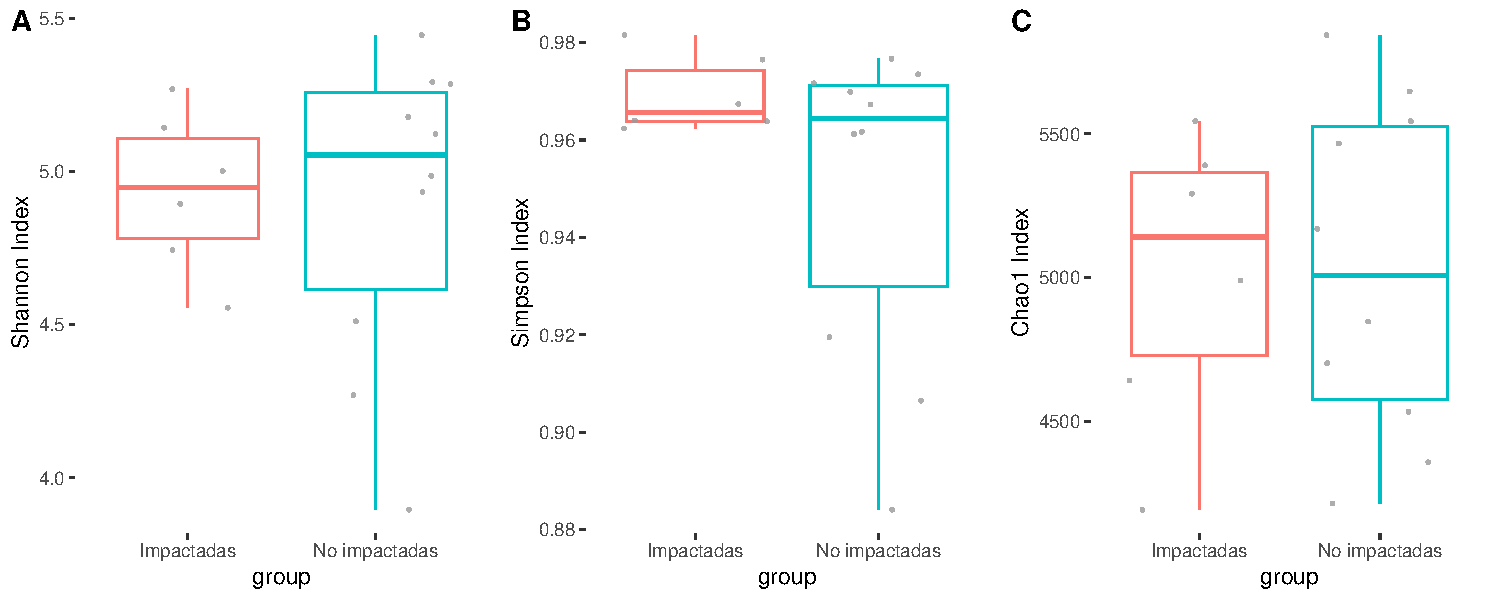
\includegraphics[width=0.9\linewidth]{images/pipeline/diversity_boxplot.pdf}
    \caption{Gráfico de cajas y bigotes de los índices de diversidad calculados para cada grupo ingresado}
    \label{fig:pipeline-diversity_boxplot}
\end{figure}

\subsubsection{Predicción funcional}
Este módulo solo se ejecutará si el parámetro \textit{functional\_prediction.run} es ``ON'' en el archivo de configuración. 
Para poder ejecutar la diferenciación entre grupos se requiere que el usuario haya ingresado esta información en el archivo de metadata.

La predicción funcional se realizará mediante la herramienta PICRUSt2. 
Para disminuir los tiempos de ejecución, se realizará la predicción por muestra y luego mediante un script en python se unirán los resultados en un solo archivo.
Para la búsqueda de vías metabólicas que presentan diferencias significativas entre grupos se utilizará la herramienta Lefse con un valor de normalización de 1.000.000.

El output de este módulo es una carpeta llamada \textit{functional\_prediction} que contiene los siguientes directorios:
\begin{itemize}
    \item \textit{picrust2\_out}: Directorio con los resultados de la predicción funcional por muestra. Contiene los siguientes directorios:
    \begin{itemize}
        \item \textit{EC\_metagenome\_out}: Directorio con los resultados de la predicción de las enzimas EC.
        \item \textit{KO\_metagenome\_out}: Directorio con los resultados de la predicción de los genes KO.
        \item \textit{Pathways\_out}: Directorio con los resultados de la predicción de las vías metabólicas.
    \end{itemize}
    \item \textit{KO.csv}: Archivo resumen con los resultados de la predicción de los genes KO para todas las muestras.
    \item \textit{EC.csv}: Archivo resumen con los resultados de la predicción de las enzimas EC para todas las muestras.
    \item \textit{Pathways.csv}: Archivo resumen con los resultados de la predicción de las vías metabólicas para todas las muestras.
    \item Gráfico de barras con vías metabólicas que presentan diferencias significativas entre grupos
    \end{itemize}

A continuación se presenta el gráfico generado donde se presentan las vías metabólicas que presentan diferencias (obtenidas mediante la herramienta LefSE) significativas entre los dos grupos ingresados  (Figura~\ref{fig:pipeline-lefse}).
    \begin{figure}[H]
        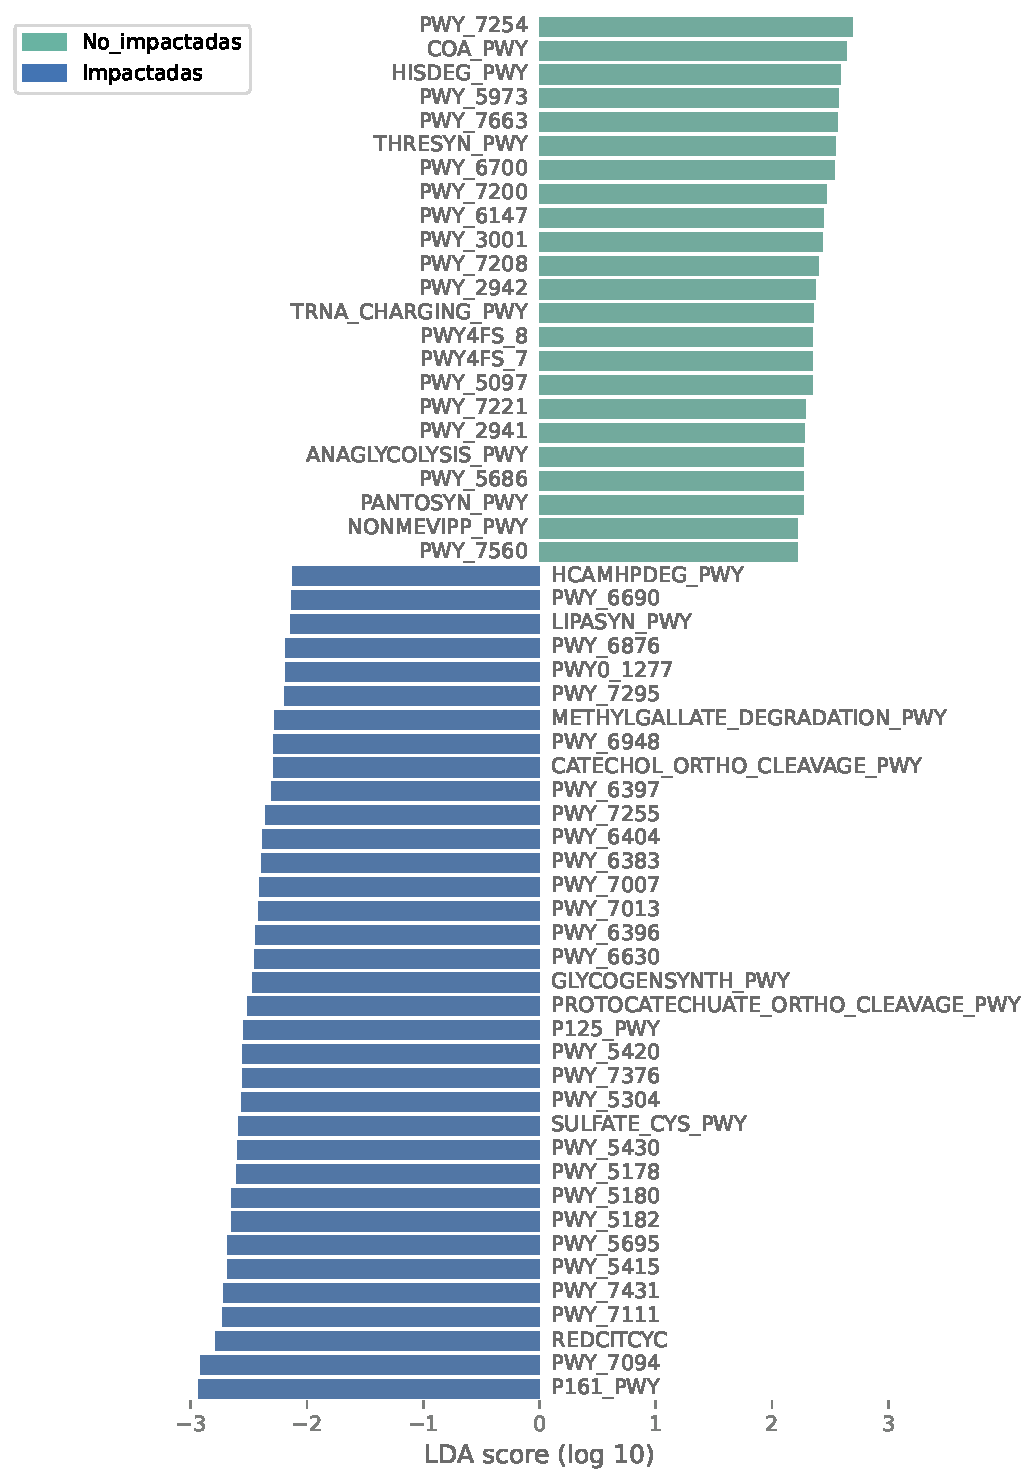
\includegraphics[width=0.7\linewidth]{images/pipeline/lefse_plot.pdf}
        \caption{Barra de navegación}
        \label{fig:pipeline-lefse}
    \end{figure}
\subsubsection{Ejecución del flujo de trabajo}\label{pipeline:how_to_run}
%https://www.ncbi.nlm.nih.gov/refseq/targetedloci/16S_process/
%%mkdir db db/taxdb
% wget https://ftp.ncbi.nlm.nih.gov/blast/db/16S_ribosomal_RNA.tar.gz && tar -xzvf 16S_ribosomal_RNA.tar.gz -C db
% wget https://ftp.ncbi.nlm.nih.gov/blast/db/taxdb.tar.gz && tar -xzvf taxdb.tar.gz -C db/taxdb
%%
Para ejecutar el flujo de trabajo se debe descargar el ejecutable de Nextflow desde su página oficial\footnote{https://www.nextflow.io/}. 
Además se requiere tener instalado conda para gestionar la instalación de paquetes y herramientas.

Para ejecutar el flujo de trabajo se debe ingresar el siguiente comando en la terminal:
\begin{verbatim}
    nextflow run nanotax-pipeline -profile conda -params-file params.yml

\end{verbatim}
El archivo \textit{params.yml} es el archivo de configuración que contiene los parámetros necesarios para la ejecución del flujo de trabajo (descrito en la sección~\ref{subsection:conf_file}).

La descarga de la base de datos de 16S de Genbank se puede realizar mediante el FTP de NCBI\footnote{ftp://ftp.ncbi.nlm.nih.gov/blast/db/16S\_ribosomal\_RNA.tar.gz}.

Se recomienda usar la opción \textit{-resume} para reanudar la ejecución en caso de que se haya interrumpido.

% \hl{Desarrollo de contenedores o conda enviroments}
% Para la reproducibilidad del flujo de trabajo se cuenta con dos \hl{executers}: Conda y \hl{Singularity}    .

\subsubsection{Tiempos de ejecución y requerimientos computacionales}



% \newpage
% \section{Aplicación Web}
% Se desarrollo una aplicación web mediante Vue3, FastAPI y PostgreSQL que permite al usuario subir sus archivos de secuenciación y metadata. 
% Con esto el usuario puede abstraerse de tener conocimiento en línea de comando o ejecución de heramientas bioinformaticas y/o flujos de trabajo, 
% ya que mediante la interfaz web el usuario solo debe seleccionar los análisis que desea realizar.
% La información ingresada por el usuario es guardada en la base de datos y mediante un script se generan los parámetros necesarios para la ejecución del flujo de trabajo.
% Una vez el pipeline termina de ejecutarse se escriben los resultados en la base de datos. 
% La plataforma lee esta información directa de la base de datos y despliega los resultados en forma de tablas y gráficos en la sección de análisis.


% A continuación se detalla cada una de las vistas de la aplicación web y su funcionalidad.
% % \subsection{Middleware}
% % \subsection{Security}

% \subsection{Login}
% Al ingresar en la página de Login, el usuario deberá ingresar su nombre de usuario y contraseña.
% En caso de que los datos sean correctos será redireccionado a la página de proyectos (Ver sección \ref{projects}).
% En caso de que los datos sean incorrectos se mostrará un mensaje de error \textit{“Usuario o contraseña incorrectos”} y deberá ingresar sus credenciales nuevamente.


% \begin{figure}[ht]
%     \centering
%     \begin{subfigure}[b]{0.45\textwidth}
%         \centering
%         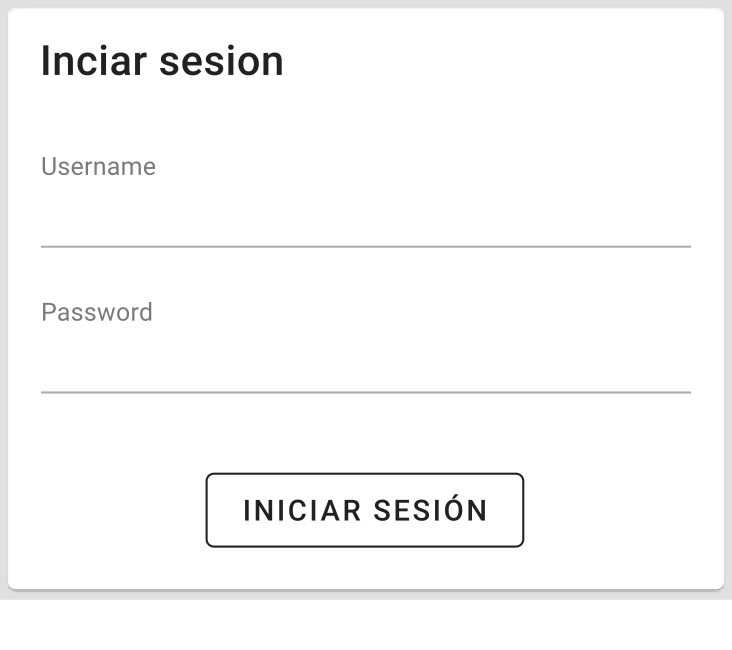
\includegraphics[width=\textwidth]{images/app/login.png}
%         \caption{Vista de inicio de sesión por defecto \newline}
%         \label{fig:app-login_default}
%     \end{subfigure}
%     \hfill
%     \begin{subfigure}[b]{0.45\textwidth}
%         \centering
%         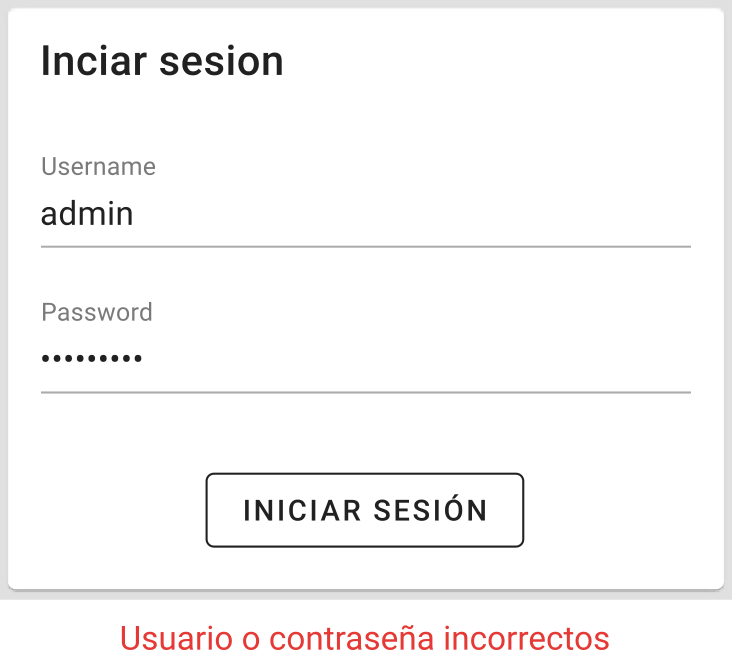
\includegraphics[width=\textwidth]{images/app/login-error.png}
%         \caption{Vista de inicio de sesión con mensaje de error al ingresar credenciales inválidas}
%         \label{fig:app-login_error}
%     \end{subfigure}
%     \caption{Vista de Inicio de sesión}
%     \label{fig:app-login}
% \end{figure}

% % \hl{Registrarse - vista}
% \subsection{Navbar}
% Una vez que el usuario inicia sesión, va a poder visualizar la barra de navegación de la plataforma en la parte superior de la página. 
% % La plataforma cuenta con las siguientes secciones en la barra de navegación:
% % \begin{itemize}
% %     \item \textit{Results}
% %     \item \textit{New analyses}
% %     \item \textit{Change password}: Cambiar contraseña
% %     \item \textit{Log out}: Cerrar sesión en la plataforma
% % \end{itemize}
% \begin{figure}[H]
%     
\includegraphics[width=1\linewidth]{images/app/navbar.png}
%     \caption{Barra de navegación}
%     \label{fig:app-nabvar}
% \end{figure}

% A continuación se describen las funcionalidades de cada una de las secciones de la barra de navegación:

% \subsection{Cambio de contraseña}
% Una vez que el usuario validó sus credenciales va a poder acceder a la vista de cambio de contraseña a través de la barra de navegación (Figura~\ref{fig:app-change-psw_default}).



% Para realizar el cambio de contraseña, deberá ingresar su contraseña actual y su nueva contraseña dos veces.
% En caso de que la contraseña sea cambiada con éxito se mostrará el mensaje \textit{“Contraseña cambiada con exito“} (Figura~\ref{fig:app-change-psw-success}).


% \begin{figure}[H]
%     \centering
%     \begin{subfigure}[b]{0.45\textwidth}
%         \centering
%         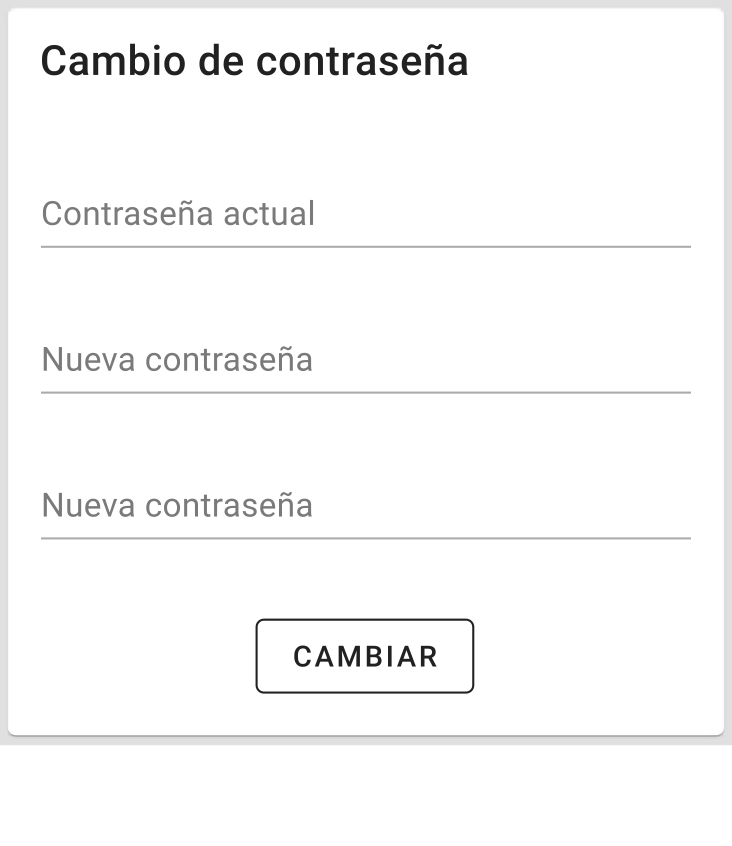
\includegraphics[width=\textwidth]{images/app/change-psw-def.png}
%         \caption{Vista de cambio de contraseña por defecto \newline}
%         \label{fig:app-change-psw_default}
%     \end{subfigure}
%     \hfill
%     \begin{subfigure}[b]{0.45\textwidth}
%         \centering
%         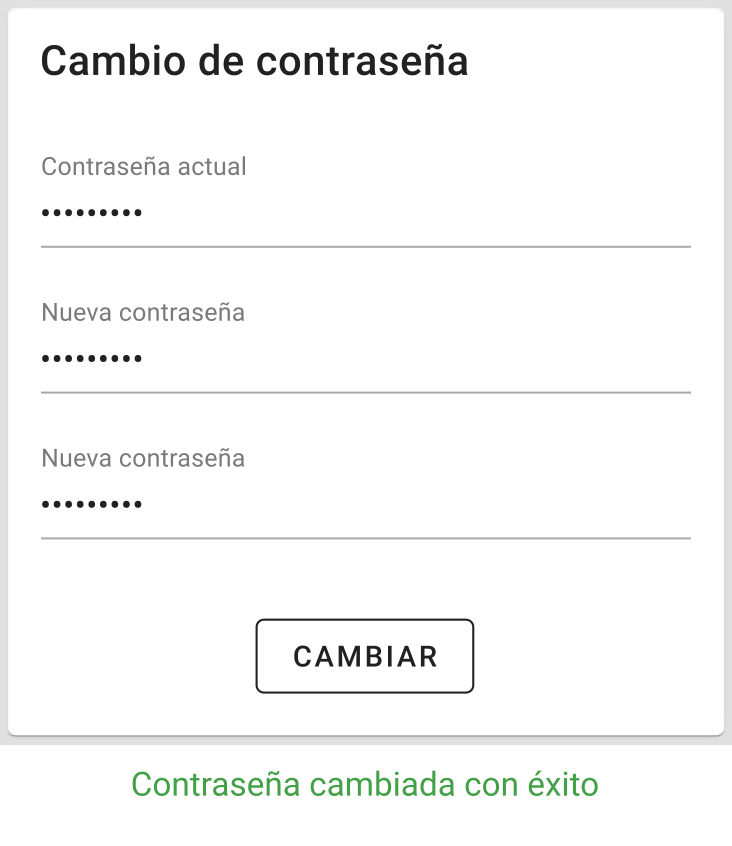
\includegraphics[width=\textwidth]{images/app/change-psw-sucess.png}
%         \caption{Vista de cambio de contraseña realizado con exito}
%         \label{fig:app-change-psw-success}
%     \end{subfigure}
%     % \caption{Vista de Cambio de contraseña (I)}
%     \label{fig:app-change-psw-1}
% \end{figure}
% En caso de que la contraseña actual sea incorrecta se mostrará el mensaje de error  \textit{“Contraseña incorrecta”} (Figura~\ref{fig:app-change-psw_error-1}).
% En caso de que las contraseñas nuevas no coincidan se mostrará el mensaje de error \textit{“Las contraseñas no coinciden”} (Figura~\ref{fig:app-change-psw_error-2})
% \begin{figure}[H]
%     \centering
%     \begin{subfigure}[b]{0.45\textwidth}
%         \centering
%         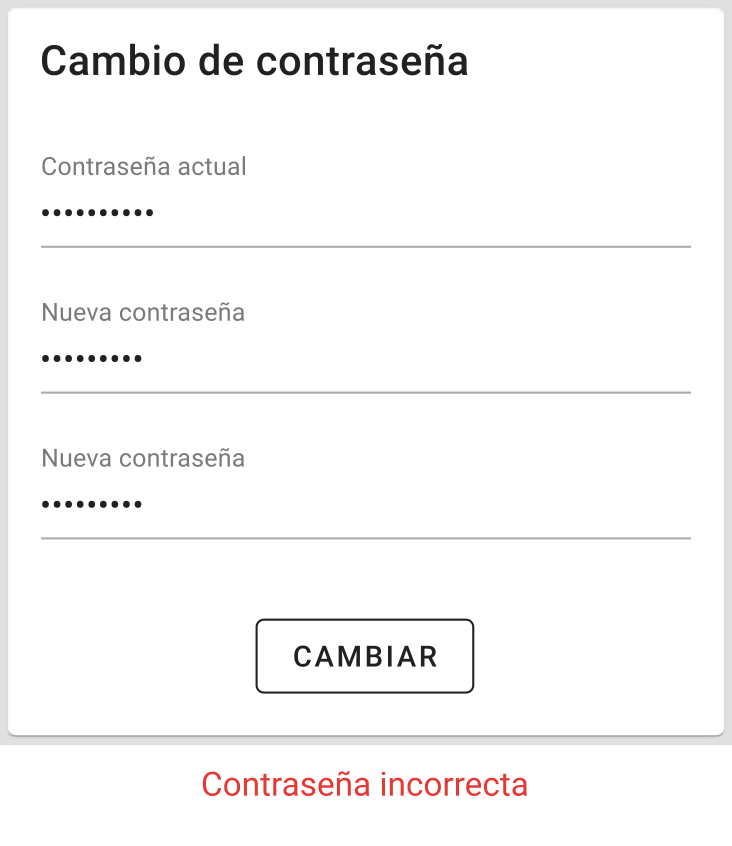
\includegraphics[width=\textwidth]{images/app/change-psw-error1.png}
%         \caption{Vista de cambio de contraseña al ingresar contraseña incorrecta}
%         \label{fig:app-change-psw_error-1}
%     \end{subfigure}
%     \hfill
%     \begin{subfigure}[b]{0.45\textwidth}
%         \centering
%         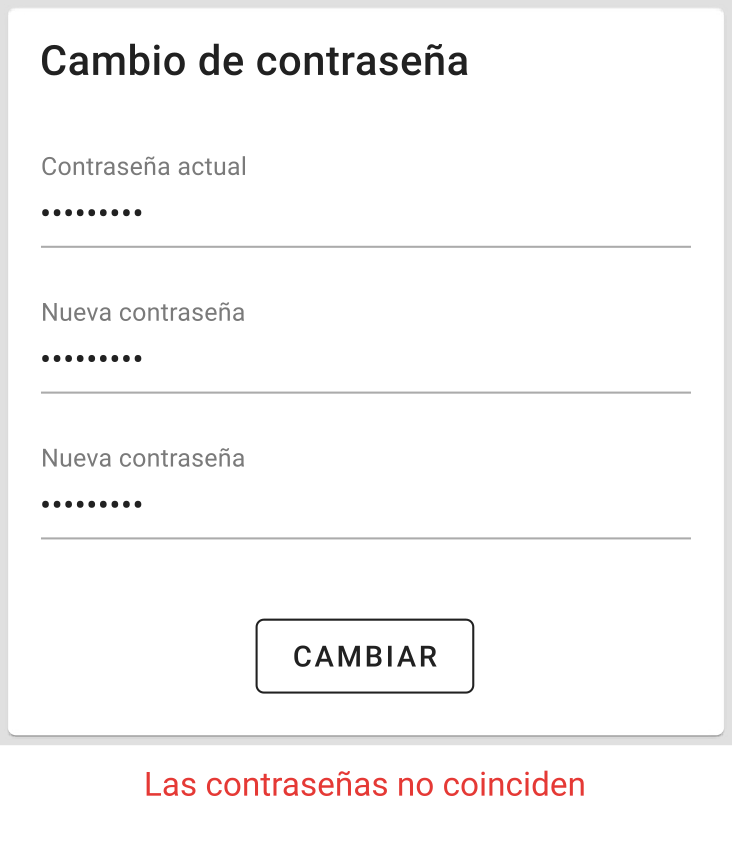
\includegraphics[width=\textwidth]{images/app/change-psw-error2.png}
%         \caption{Vista de cambio de contraseña al ingresar contraseñas que no coinciden}
%         \label{fig:app-change-psw_error-2}
%     \end{subfigure}
%     % \caption{Vista de Cambio de contraseña (II)}
%     \label{fig:app-change-psw-2}
% \end{figure}

% En el caso de que la nueva contraseña no cumpla los críterios de seguridad (longitud mínima de 8 caracteres y al menos un número) se mostrará el mensaje de error  \textit{“La contraseña debe tener al menos 8 caracteres / La contraseña debe tener al menos un número”} (Figura~\ref{fig:app-change-psw_error-1}).
% \begin{figure}[H]
%     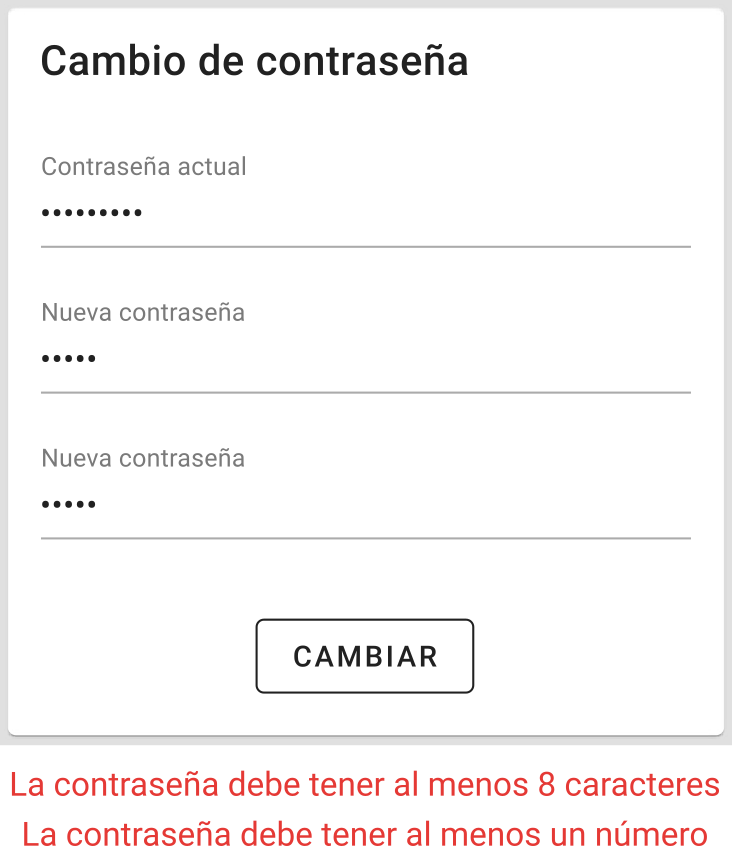
\includegraphics[width=0.45\linewidth]{images/app/change-psw-error3.png}
%     \captionsetup{justification=raggedright, width=0.45\linewidth, singlelinecheck=off}

%     % \captionsetup{width=0.45\linewidth}
%     \caption{Vista de cambio de contraseña al ingresar una nueva contraseña que no cumple con los críterios de seguridad}
%     \label{fig:app-change-psw_error-3}
% \end{figure}

% % \begin{figure}[H]
% %     \centering
% %     \begin{subfigure}[b]{0.4\textwidth}
% %         \centering
% %         \includegraphics[width=\textwidth]{images/app/chage-psw-def.png}
% %         \caption{a}
% %         \label{fig:subfig1}
% %     \end{subfigure}
% %     \hfill
% %     \begin{subfigure}[b]{0.4\textwidth}
% %         \centering
% %         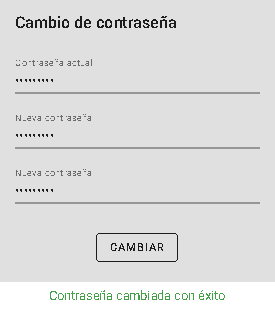
\includegraphics[width=\textwidth]{images/app/chage-psw-sucess.png}
% %         \caption{b}
% %         \label{fig:subfig2}
% %     \end{subfigure}

% %     \vskip\baselineskip

% %     \begin{subfigure}[b]{0.4\textwidth}
% %         \centering
% %         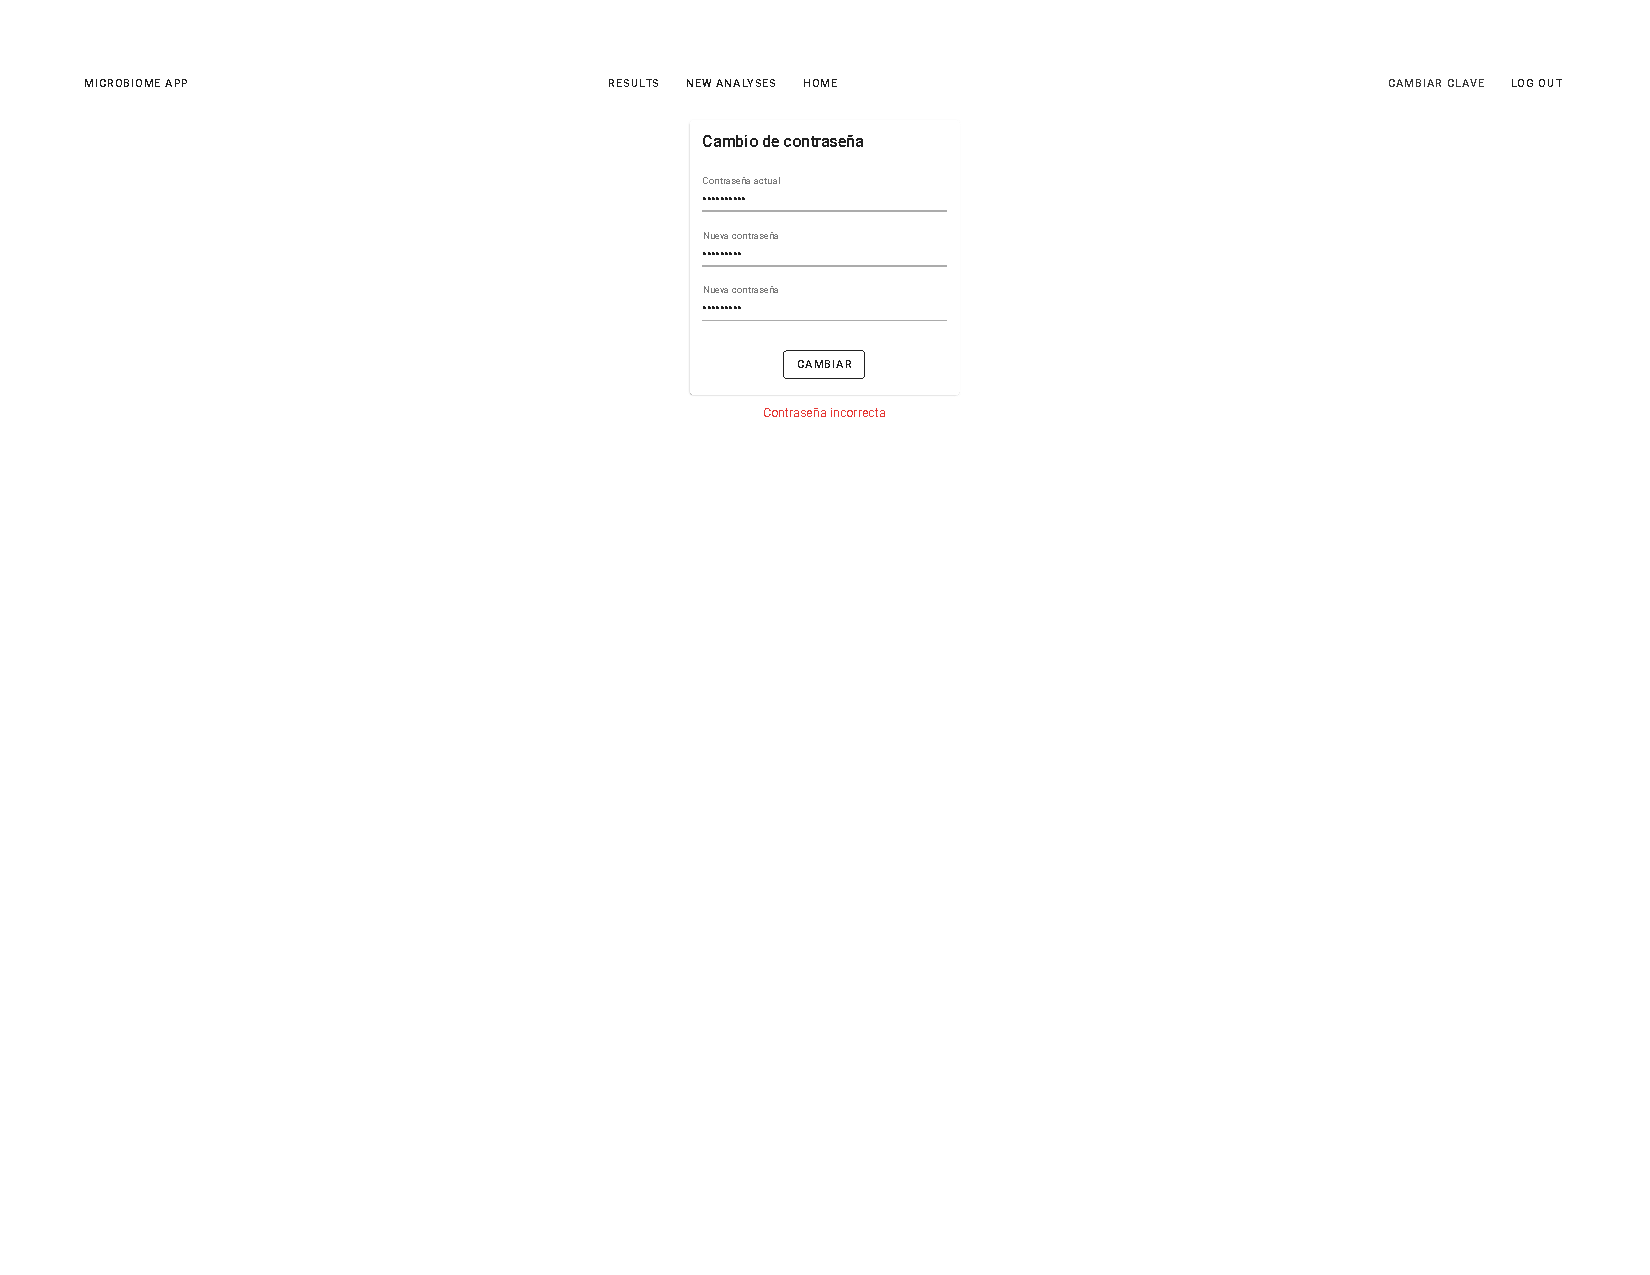
\includegraphics[width=\textwidth]{images/app/chage-psw-error1.png}
% %         \caption{c}
% %         \label{fig:subfig3}
% %     \end{subfigure}
% %     \hfill
% %     \begin{subfigure}[b]{0.4\textwidth}
% %         \centering
% %         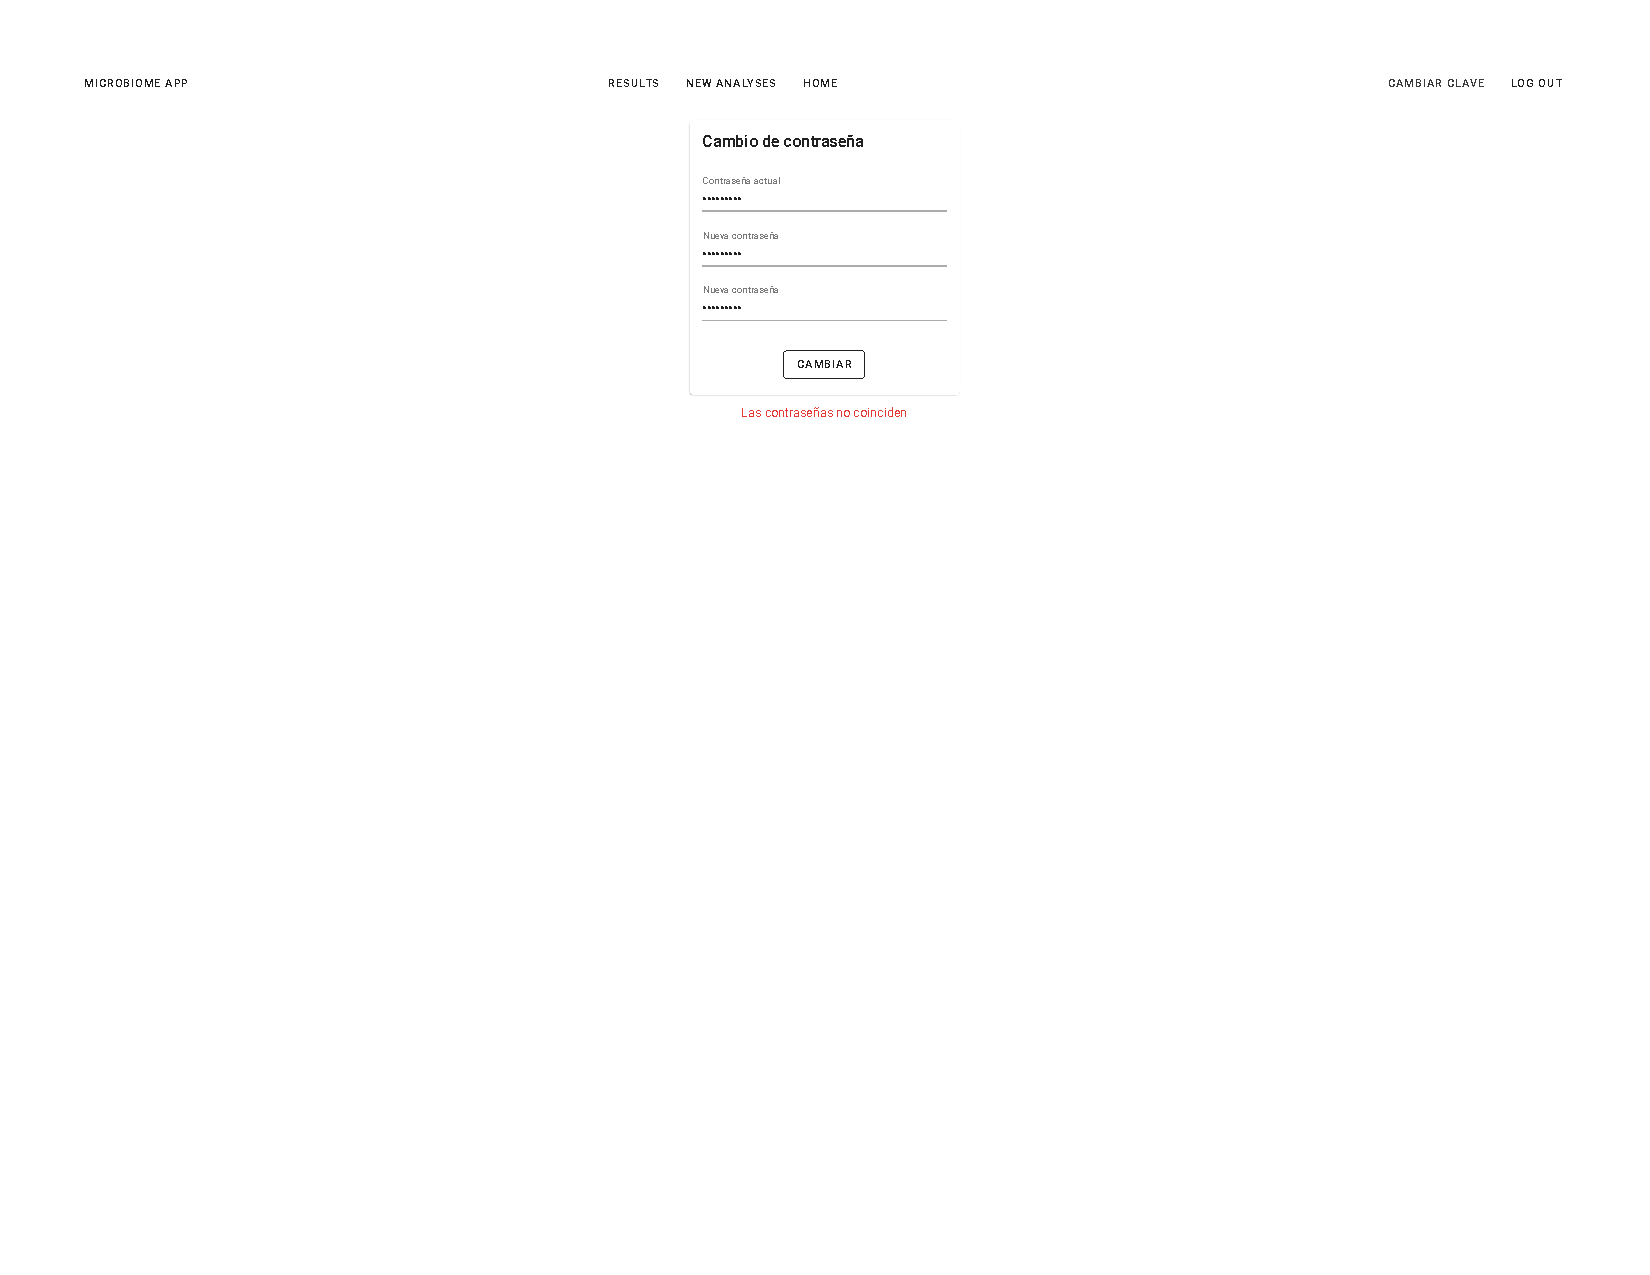
\includegraphics[width=\textwidth]{images/app/chage-psw-error2.png}
% %         \caption{d}
% %         \label{fig:subfig4}
% %     \end{subfigure}

% %     \vskip\baselineskip

% %     \begin{subfigure}[b]{0.4\textwidth}
% %         \centering
% %         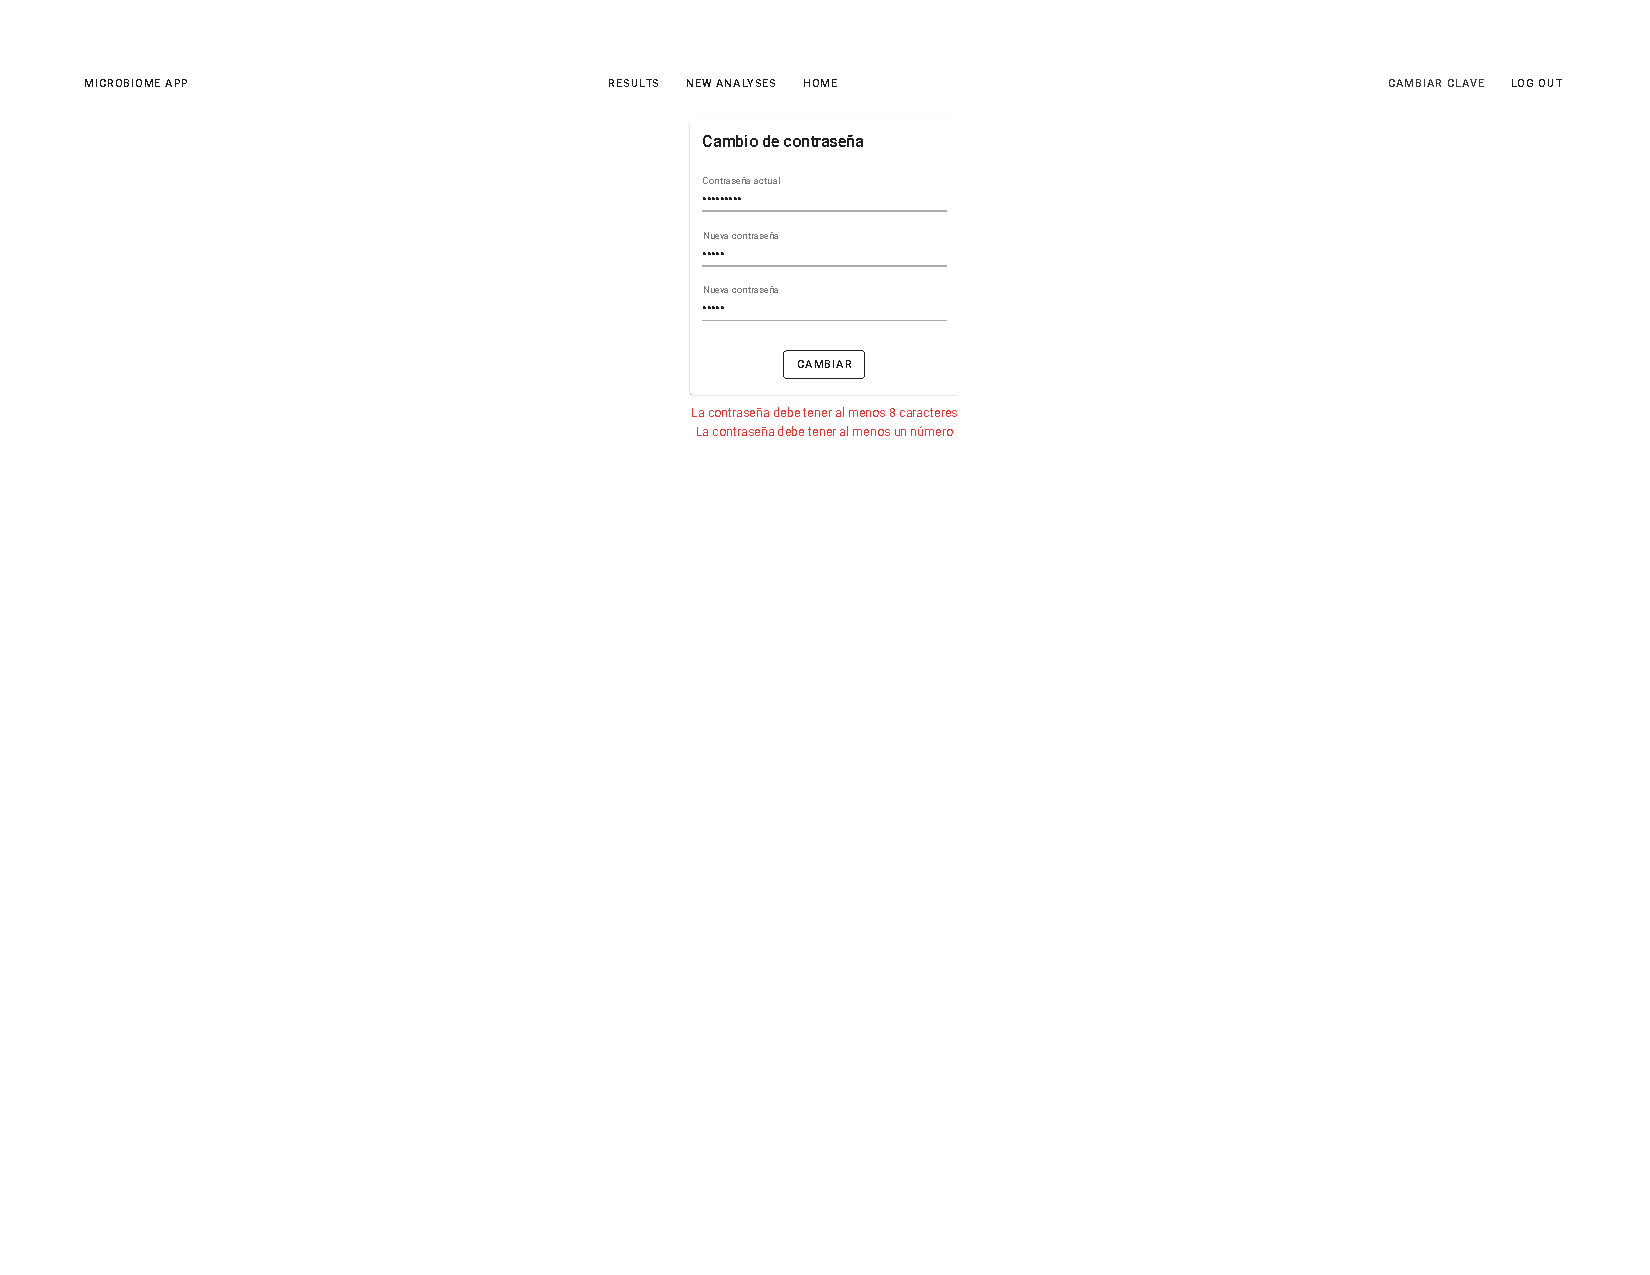
\includegraphics[width=\textwidth]{images/app/chage-psw-error3.png}
% %         \caption{e}
% %         \label{fig:subfig5}
% %     \end{subfigure}
    
% %     \caption{Título de la figura principal}
% %     \label{fig:main}
% % \end{figure}


% \subsection{Nuevo análisis}
% En esta sección el usuario deberá ingresar la información del proyecto, datos de secuenciación, y metadata para poder realizar los análisis. 
% El usuario deberá rellenar la información básica del proyecto como, nombre, descripción, tipo de archivos y mediante un archivo en formato (XLXS) deberá ingresar la información de las muestras. %, como nombre de archivo, nombre de la muestra, barcode (opcional) y grupo (opcional).
% Los datos de secuenciación se debe subir a algún directorio del drive del usuario y se debe dar acceso a la cuenta \textit{nanotax.catg@gmail.com}.
% La figura~\ref{fig:app-new-analysis-def} presenta la vista inicial de la sección de Nuevo análisis.

% \begin{figure}[H]
%     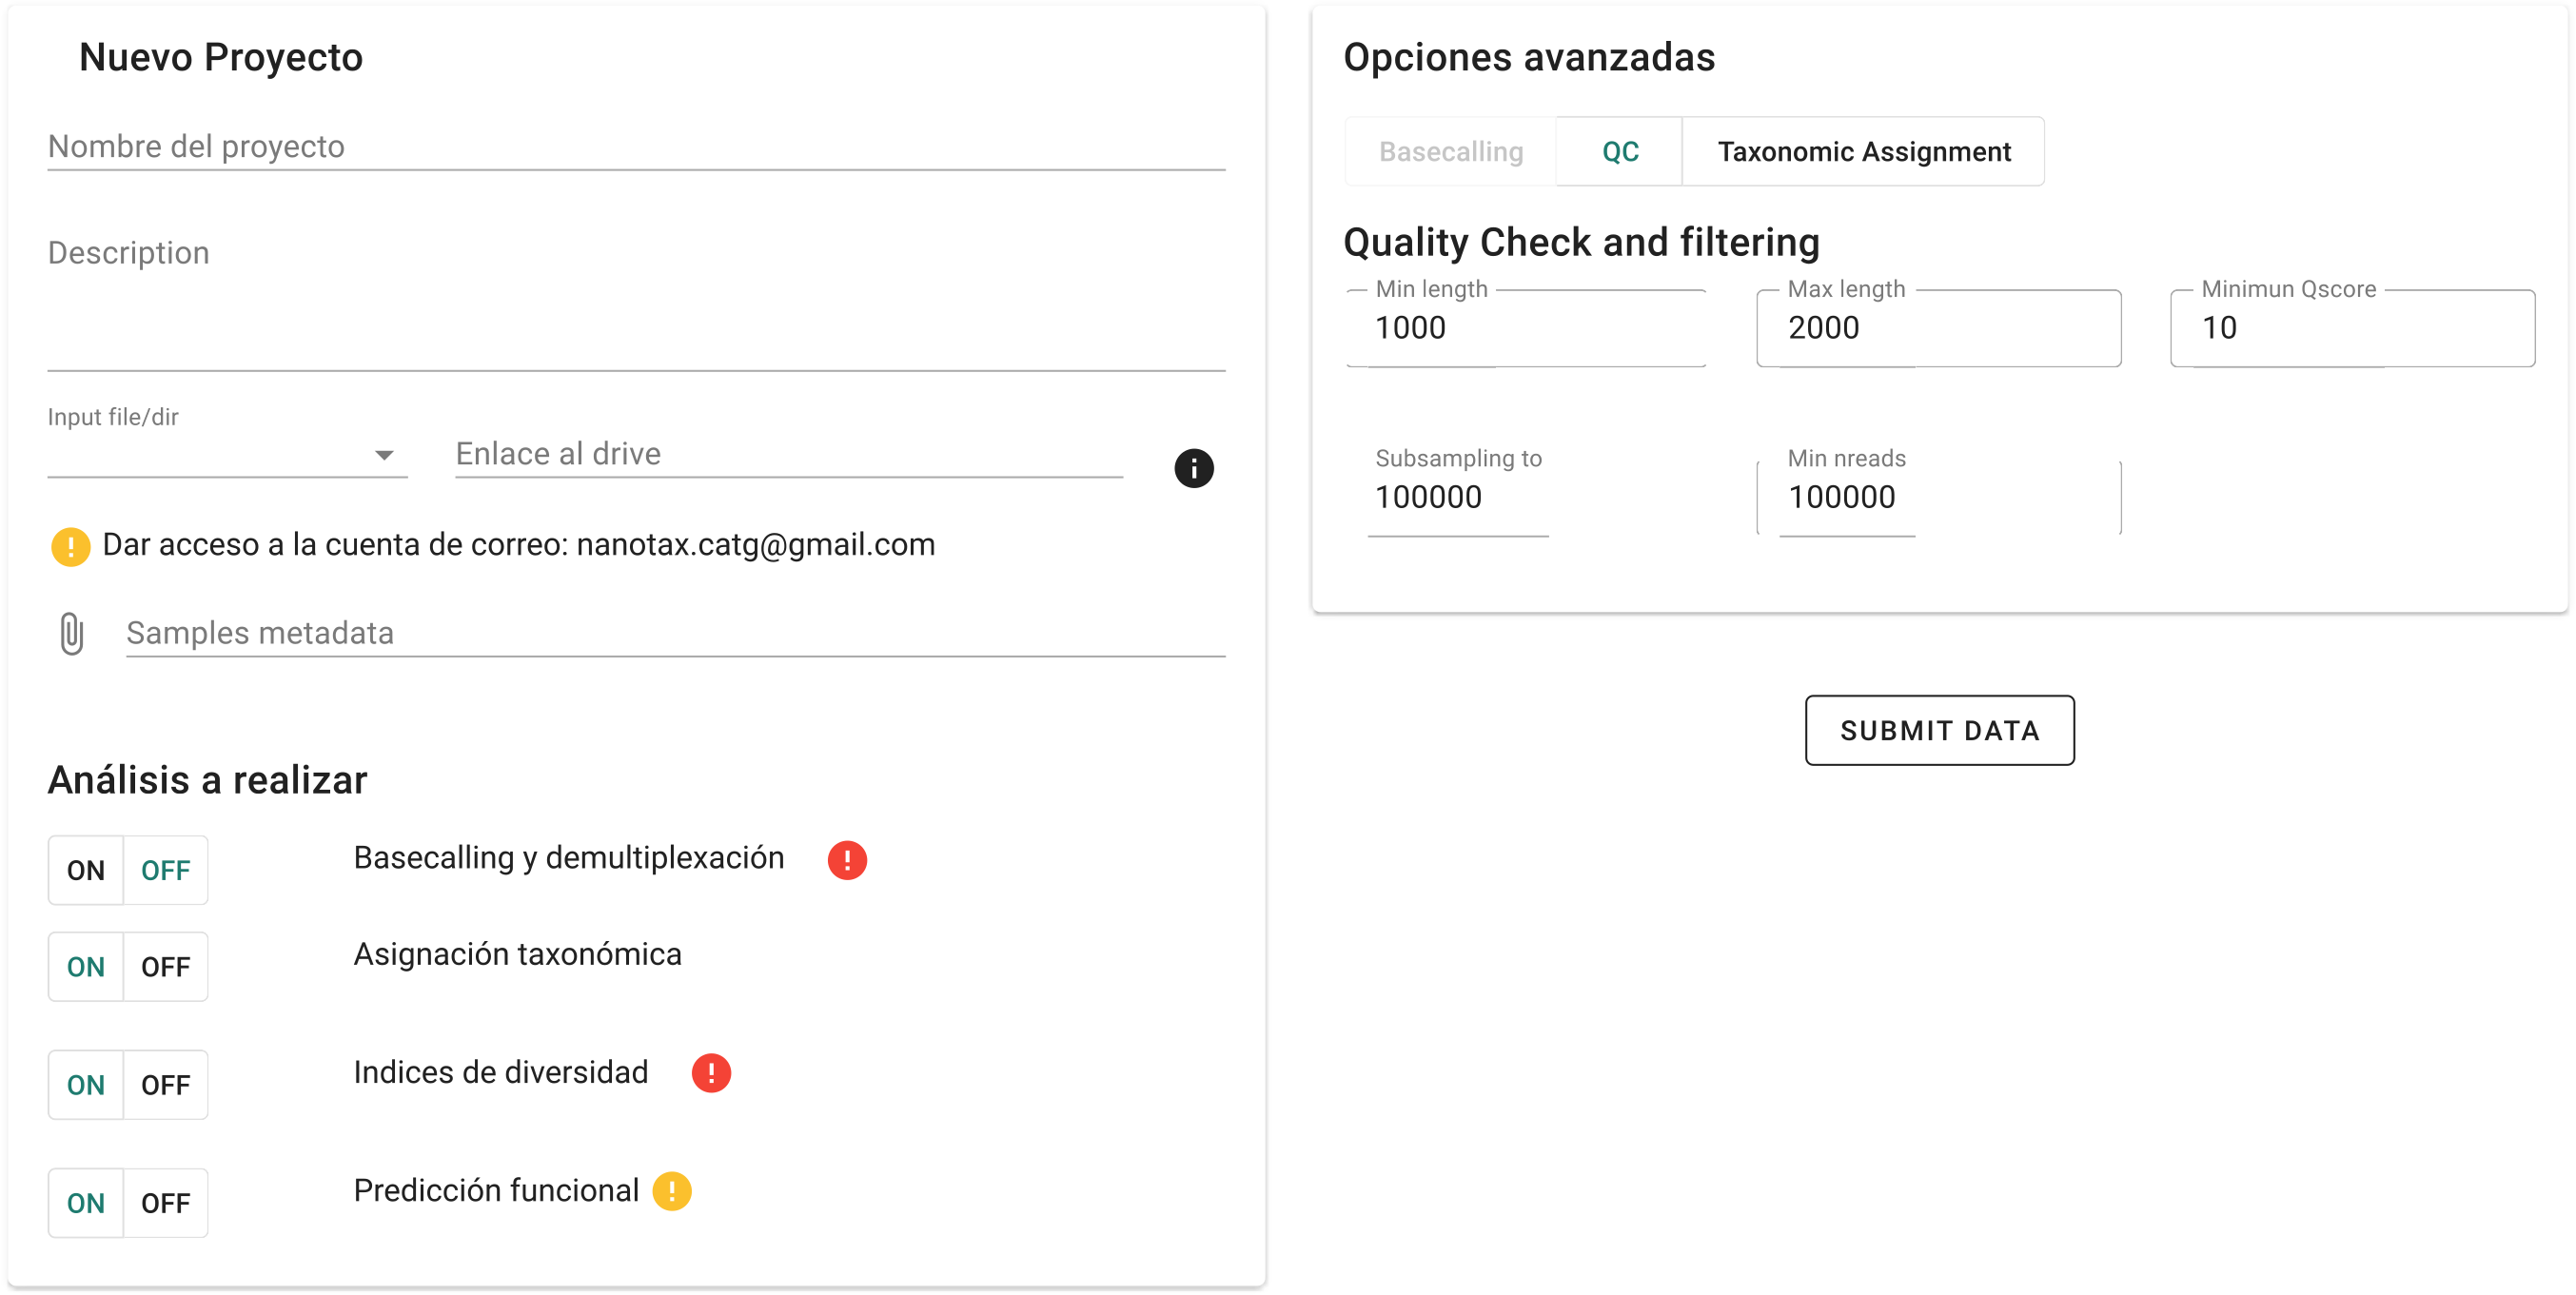
\includegraphics[width=1\linewidth]{images/app/newAnalysis/new-analysis-def.png}
%     % \captionsetup{justification=raggedright, width=0.45\linewidth, singlelinecheck=off}

%     % \captionsetup{width=0.45\linewidth}
%     \caption{Vista por defecto de Nuevo análisis}
%     \label{fig:app-new-analysis-def}
% \end{figure}


% A continuación se describen los datos que el usuario debe rellenar:

% \begin{itemize}
%     \item Nombre: Nombre del proyecto a utilizar en la plataforma (sección de visualización de proyectos y resultados).
%     \item Descripción (opcional): Descripción del proyecto, campo opcional.
%     \item Tipo de archivo a subir (POD5, FASTQ): Archivos de secuenciación que se procesarán:
%     \begin{itemize}
%         \item POD5: En caso de querer comenzar desde el proceso de basecalling y demultiplexación de las muestras.
%         \item FASTQ: En caso de querer saltarse el paso de basecalling y demultiplexación e iniciar directamente con el control de calidad y asignación taxonómica.
%     \end{itemize}
%     \item Archivo de metadata en formato XLXS con las siguientes columnas para cada muestra:
%     \begin{itemize}
%         \item file: nombre del archivo subido al drive (obligatorio)
%         \item sample: identificador de la muestra (obligatorio)
%         \item barcode (opcional): barcode que identifica la muestra (en caso de querer realizar basecalling y demultiplexación)
%         \item group (opcional): groupo al que pertenece cada muestra (en caso de querer hacer diferenciación entre grupos)
%     \end{itemize}
%     \item Análisis a realizar:
%     \begin{itemize}
%         \item Basecalling y demultiplexacion
%         \item Asignación taxonomica
%         \item Indices de diversidad
%         \item Predicción funcional
%     \end{itemize}
% \end{itemize}


% En el lado derecho de la vista se puede visualizar una sección de opciones avanzadas, donde el usuario puede modificar los parámetros por defecto en caso de que quiera modificar el comportamiento del pipeline (gigura~\ref{fig:app-new-analysis-def}). Esta información es seleccionados desde la base de datos la cual almacena los parámetros por defecto del flujo de trabajo.

% Cabe destacar que en caso de que el directorio del drive no contenga la información necesaria, el proyecto se subirá correctamente y luego pasara a un estado de datos inválidos.
% Los filtros y control de calidad se realizan siempre por lo que no aparecerá la opción en la lista de análisis.
% Por defecto basecalling y demuliplexación se encuentra deshabilitado, en caso de que el usuario desee realizar este análisis deberá seleccionarlo, y al hacerlo se desbloqueará la sección de configuración de este análisis (Figura~\ref{fig:app-new-analysis-basecallingON}).



% \begin{figure}[H]
%     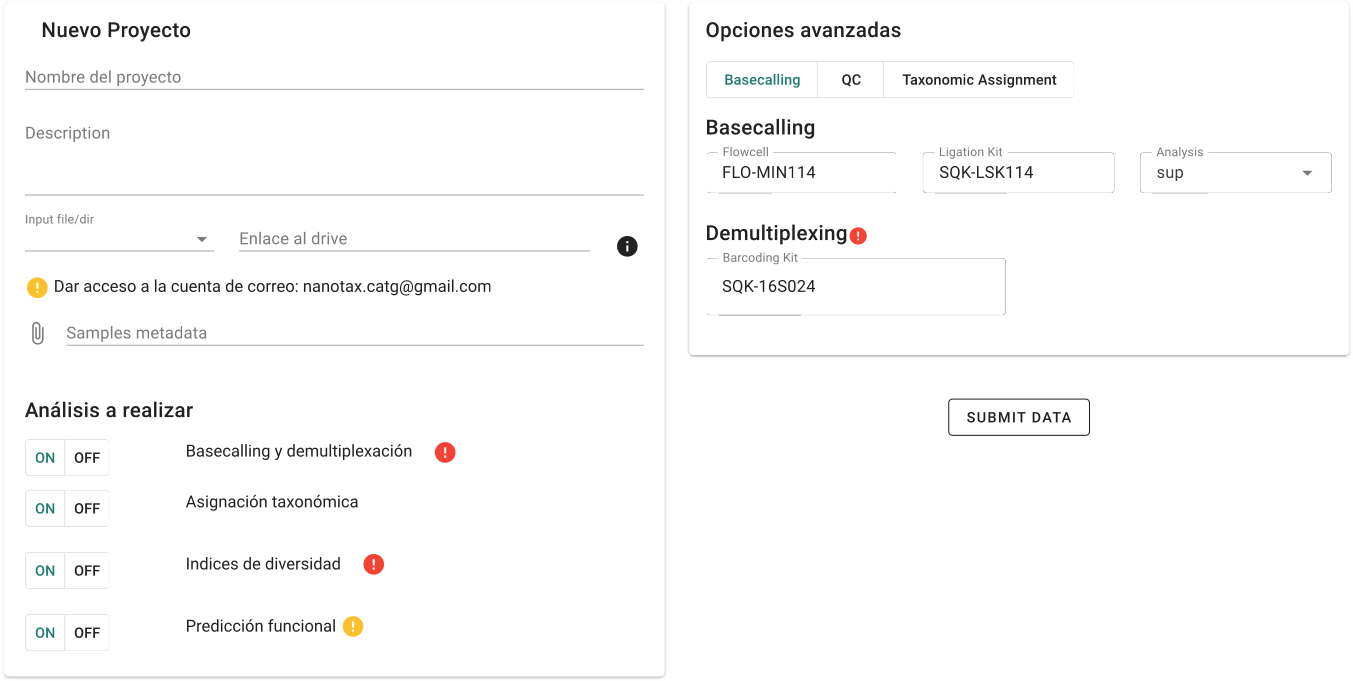
\includegraphics[width=1\linewidth]{images/app/newAnalysis/new-analysis-basecallingON.png}
%     % \captionsetup{justification=raggedright, width=0.45\linewidth, singlelinecheck=off}

%     % \captionsetup{width=0.45\linewidth}
%     \caption{Vista de Nuevo análisis habilitando la opción de basecalling y demultiplexación}
%     \label{fig:app-new-analysis-basecallingON}
% \end{figure}
% % La plataforma se encarga de verificar si el archivo de metadata cuenta con la información necesaria para realizar cada analisis. En caso de que el archivo de metadata no cuente con la información necesaria y el usuario desee realizar uno de esos analisis, se desplegara un mensaje de error al lado del análisis indicando que información se debe añadir en el archivo de metadata. Los parámetros que se pueden modificar son los siguientes:
% % \begin{itemize}
% %     \item Basecalling y demultiplexacion: Flowcell, kit de ligación y kit de barcoding utilizados durante la secuenciación. Modelo a utilizar para realizar el basecalling
% %     \item QC: Longitud mínima y máxima en pares de bases de las lecturas, calidad mínima de las lecturas y cantidad de lecturas a utilizar para los análisis posteriores(subsampleo).
% %     \item Predicción funcional: \hl{completar}
% % \end{itemize}

% % En la parte derecha del componente el usuario puede visualizar los parámetros por defecto y modificarlos en caso de que lo desee. 


% Una vez que el usuario presione al botón \textit{Subir proyecto}, la plataforma realiza un proceso de validación para verificar que toda la información subida por el usuario sea correcta. En caso de no serla, la plataforma no permitirá subir el proyecto y podrá presentar alguno de los siguientes mensajes de error:
% \begin{itemize}
%     \item En caso de no completar el nombre del proyecto o el enlace al directorio del drive ambos campos pasarán a estar en color rojo (figura ~\ref{fig:app-new-analysis-type-file-error}).
%     \item En caso de no seleccionar el tipo de archivo a subir, este campo pasará a estar en color rojo y se presentará el siguiente mensaje: \textit{Debe seleccionar el formato de los archivos de entrada} (figura ~\ref{fig:app-new-analysis-type-file-error}).
%     \item En caso de seleccionar el formato de archivo \textit{POD5} y no haber seleccionado el proceso de basecalling y demultiplexación como inicio se presentará el mensaje: \textit{Al iniciar con basecalling debe subir los archivos POD5} (figura ~\ref{fig:app-new-analysis-type-file-error}).
%     \item En caso de seleccionar el formato de archivo \textit{FASTQ} y haber seleccionado el proceso de basecalling y demultiplexación como inicio se presentará el mensaje: \textit{Al iniciar con QC o asignación taxonómica debe subir los archivos FASTQ} (figura ~\ref{fig:app-new-analysis-type-file-error}).
%     \item En caso de que el archivo de metadata no cuente con todas las columnas necesarias se pueden presentar uno o más de los siguientes mensajes de errores (figura ~\ref{fig:app-new-analysis-type-file-error}):
%     \begin{itemize}
%         \item \textit{El archivo de metadata le falta la columna file}
%         \item \textit{El archivo de metadata le falta la columna sample}
%         \item \textit{El archivo de metadata le falta la columna barcode}: Solo en caso de seleccionar basecalling y demultiplexación como inicio del pipeline.
%         \item \textit{El archivo de metadata le falta la columna group}: Solo en caso de querer realizar análisis por grupos (índices de diversidad).

%     \end{itemize}
% \end{itemize}


% \begin{figure}[H]
%     \centering
%     \begin{subfigure}[b]{0.45\textwidth}
%         \centering
%         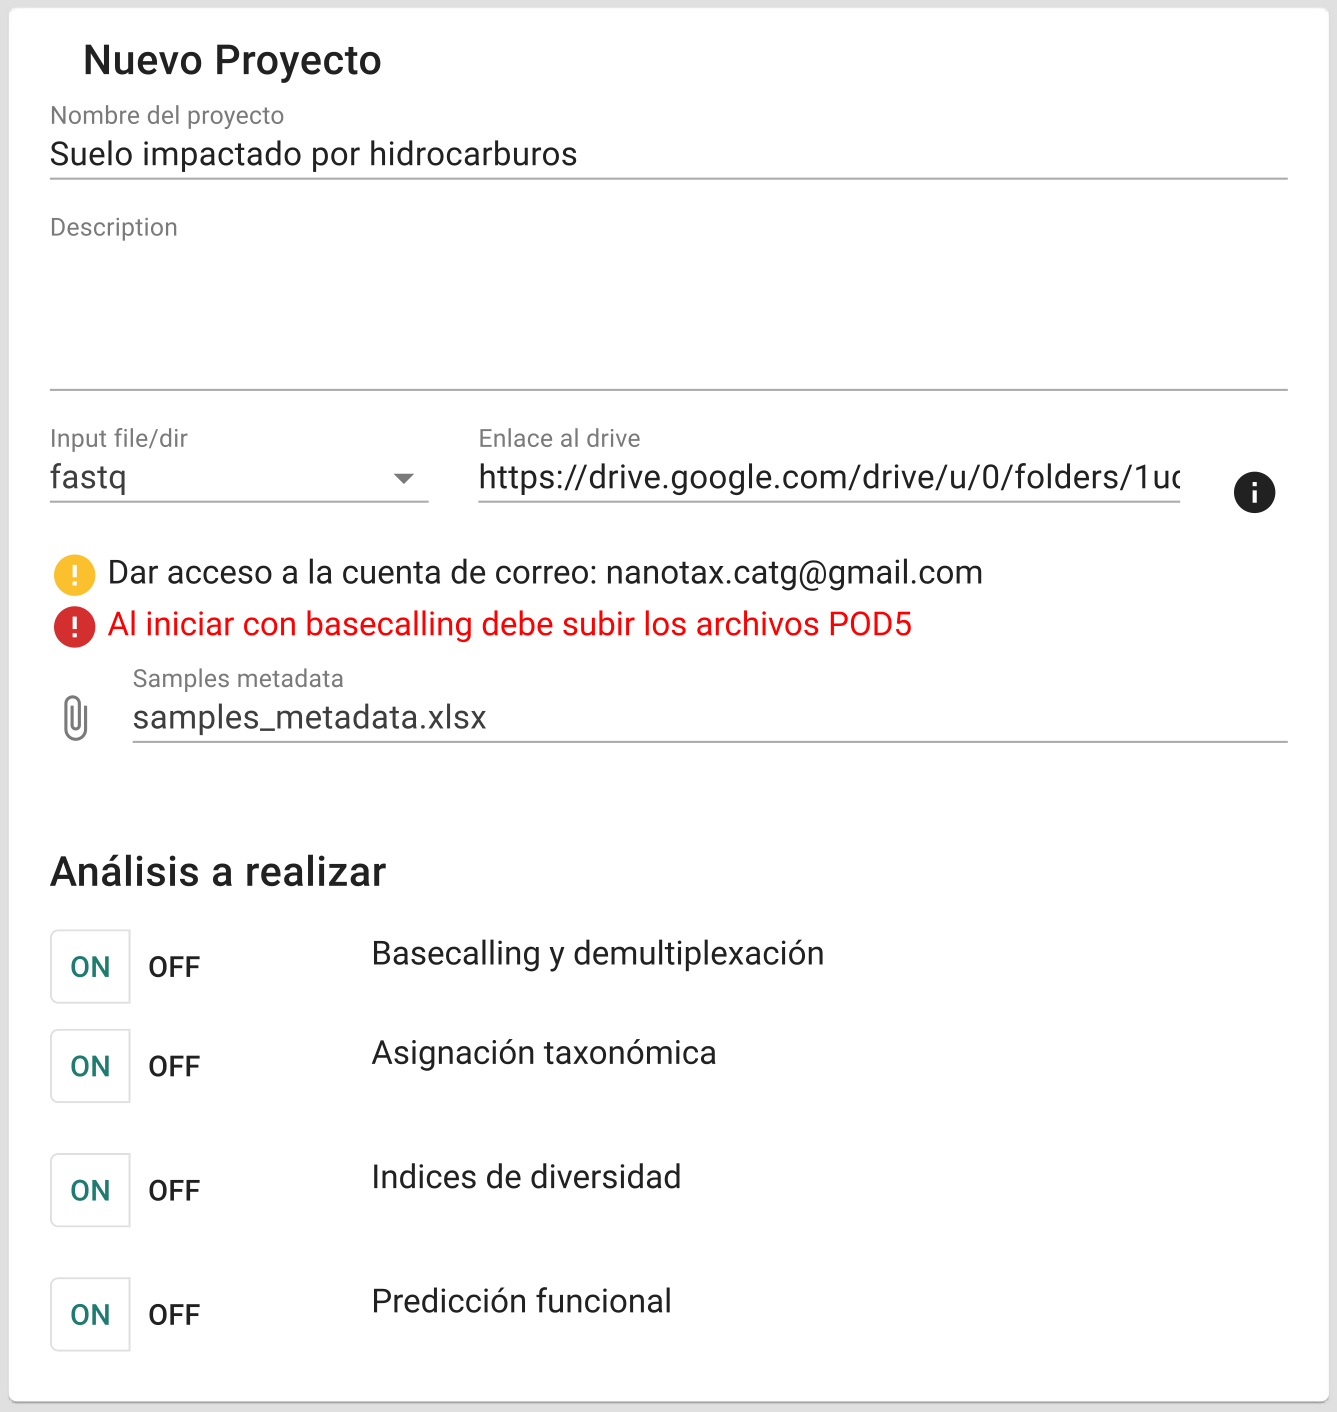
\includegraphics[width=\textwidth]{images/app/newAnalysis/pod5-error.png}
%         \caption{Vista de nuevo análisis: Error al seleccionar el tipo del archivo}
%         \label{fig:app-new-analysis-pod5-error}
%     \end{subfigure}
%     \hfill
%     \begin{subfigure}[b]{0.45\textwidth}
%         \centering
%         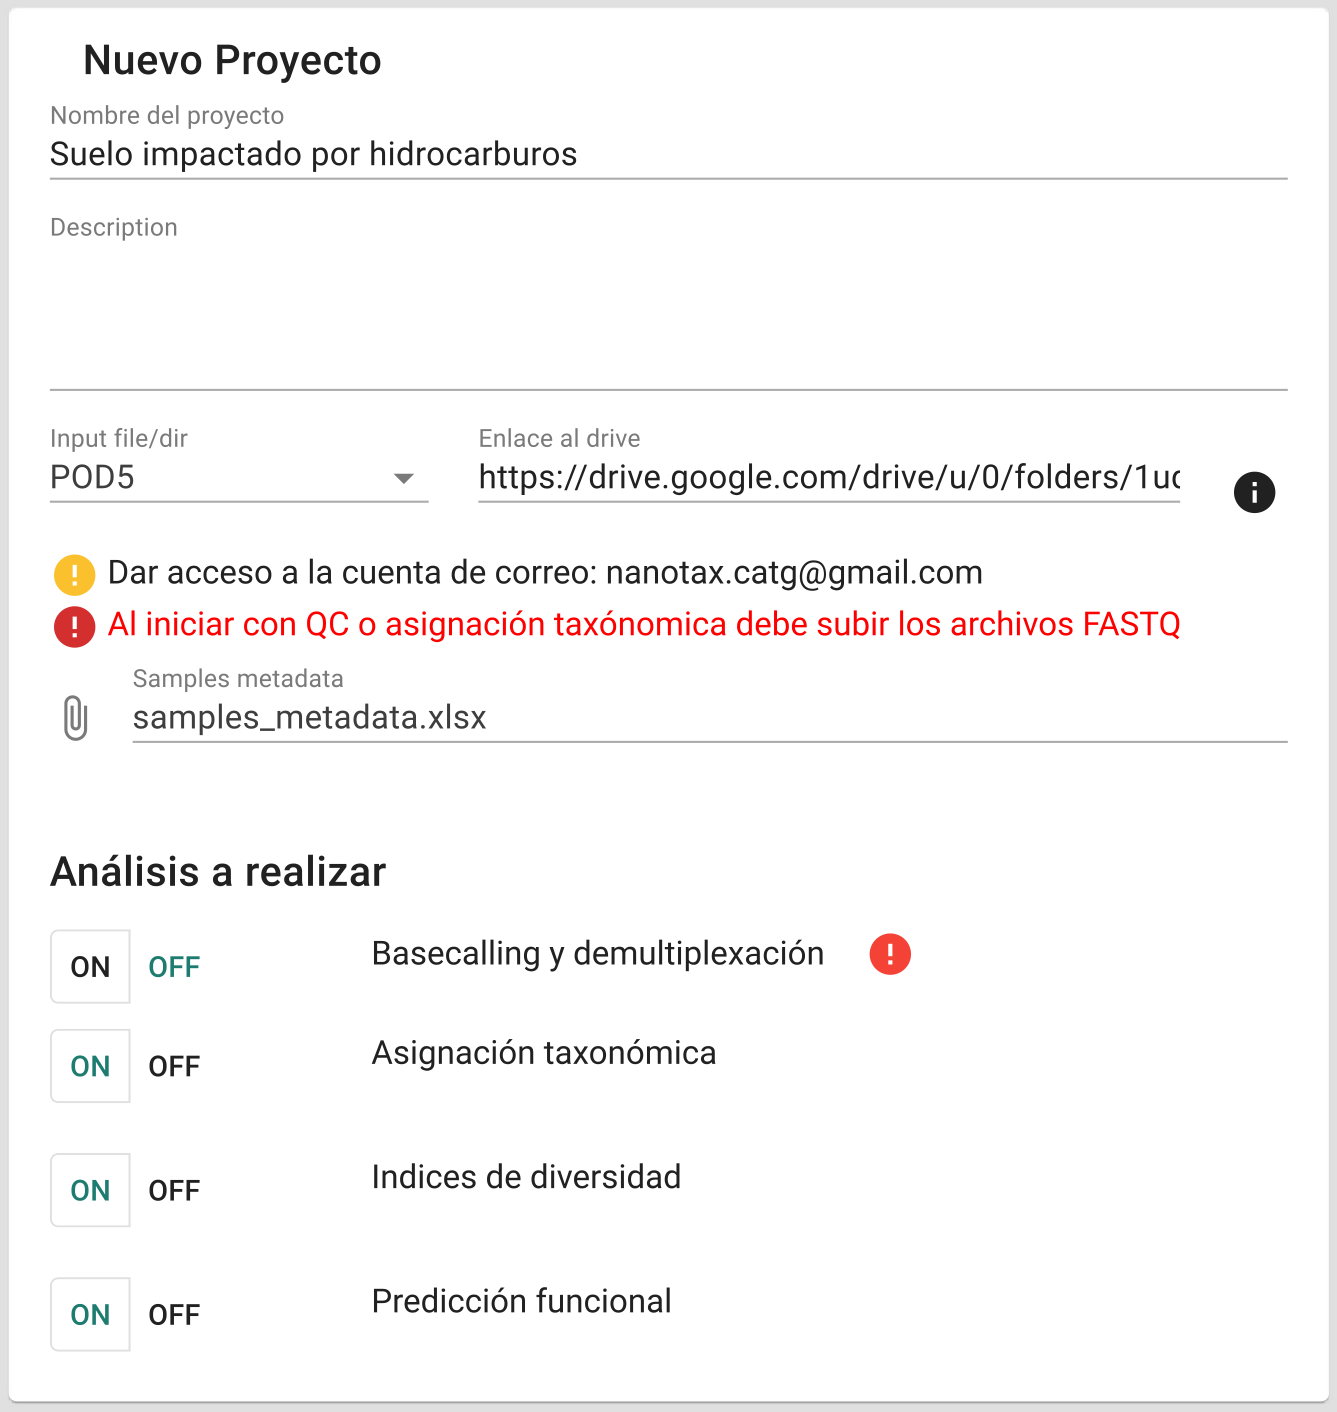
\includegraphics[width=\textwidth]{images/app/newAnalysis/fastq.png}
%         \caption{Vista de nuevo análisis: Error al seleccionar el tipo del archivo}
%         \label{fig:app-new-analysis-fastq-error}
%     \end{subfigure}
%     \caption{Vista de nuevo análisis: Error al seleccionar el tipo del archivo}
%     \label{fig:app-new-analysis-type-file-error}
% \end{figure}



% \begin{figure}[H]
%     \centering
%     \begin{subfigure}[b]{0.45\textwidth}
%         \centering
%         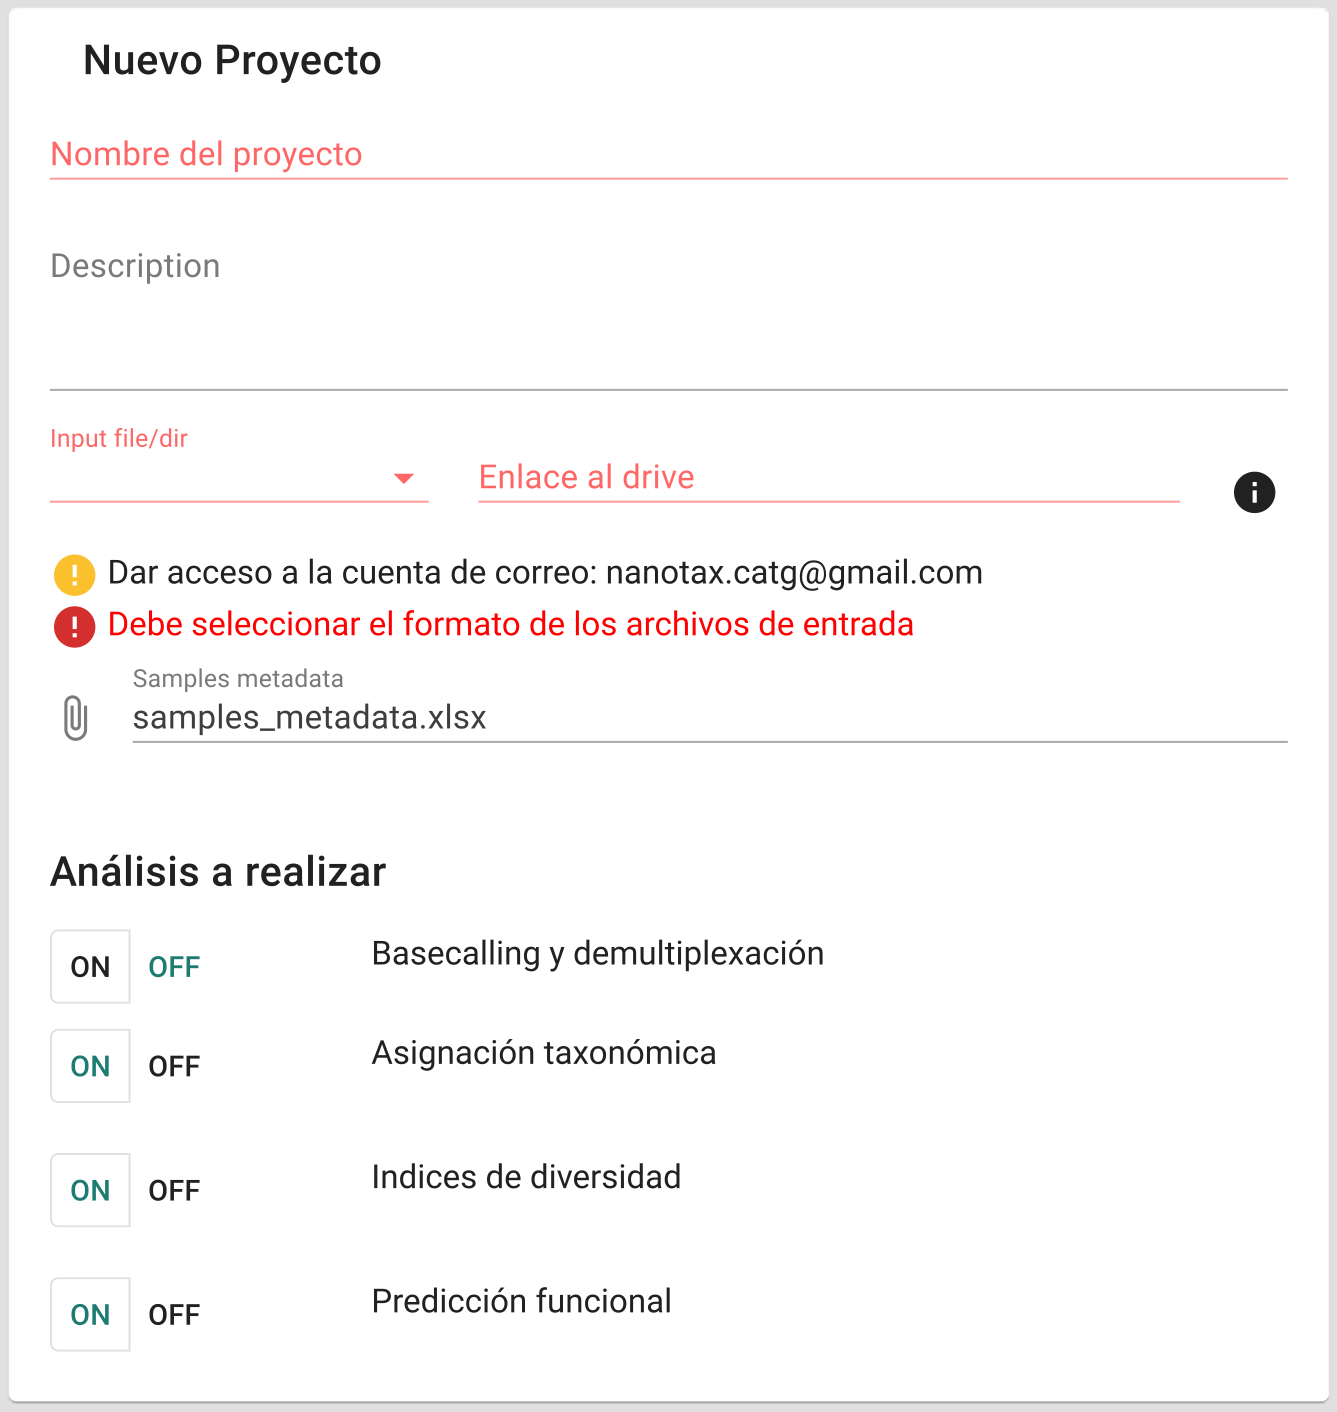
\includegraphics[width=\textwidth]{images/app/newAnalysis/errors1.png}
%         \caption{Vista de nuevo análisis: Errores por falta de información}
%         \label{fig:app-new-analysis-nodata-error}
%     \end{subfigure}
%     \hfill
%     \begin{subfigure}[b]{0.45\textwidth}
%         \centering
%         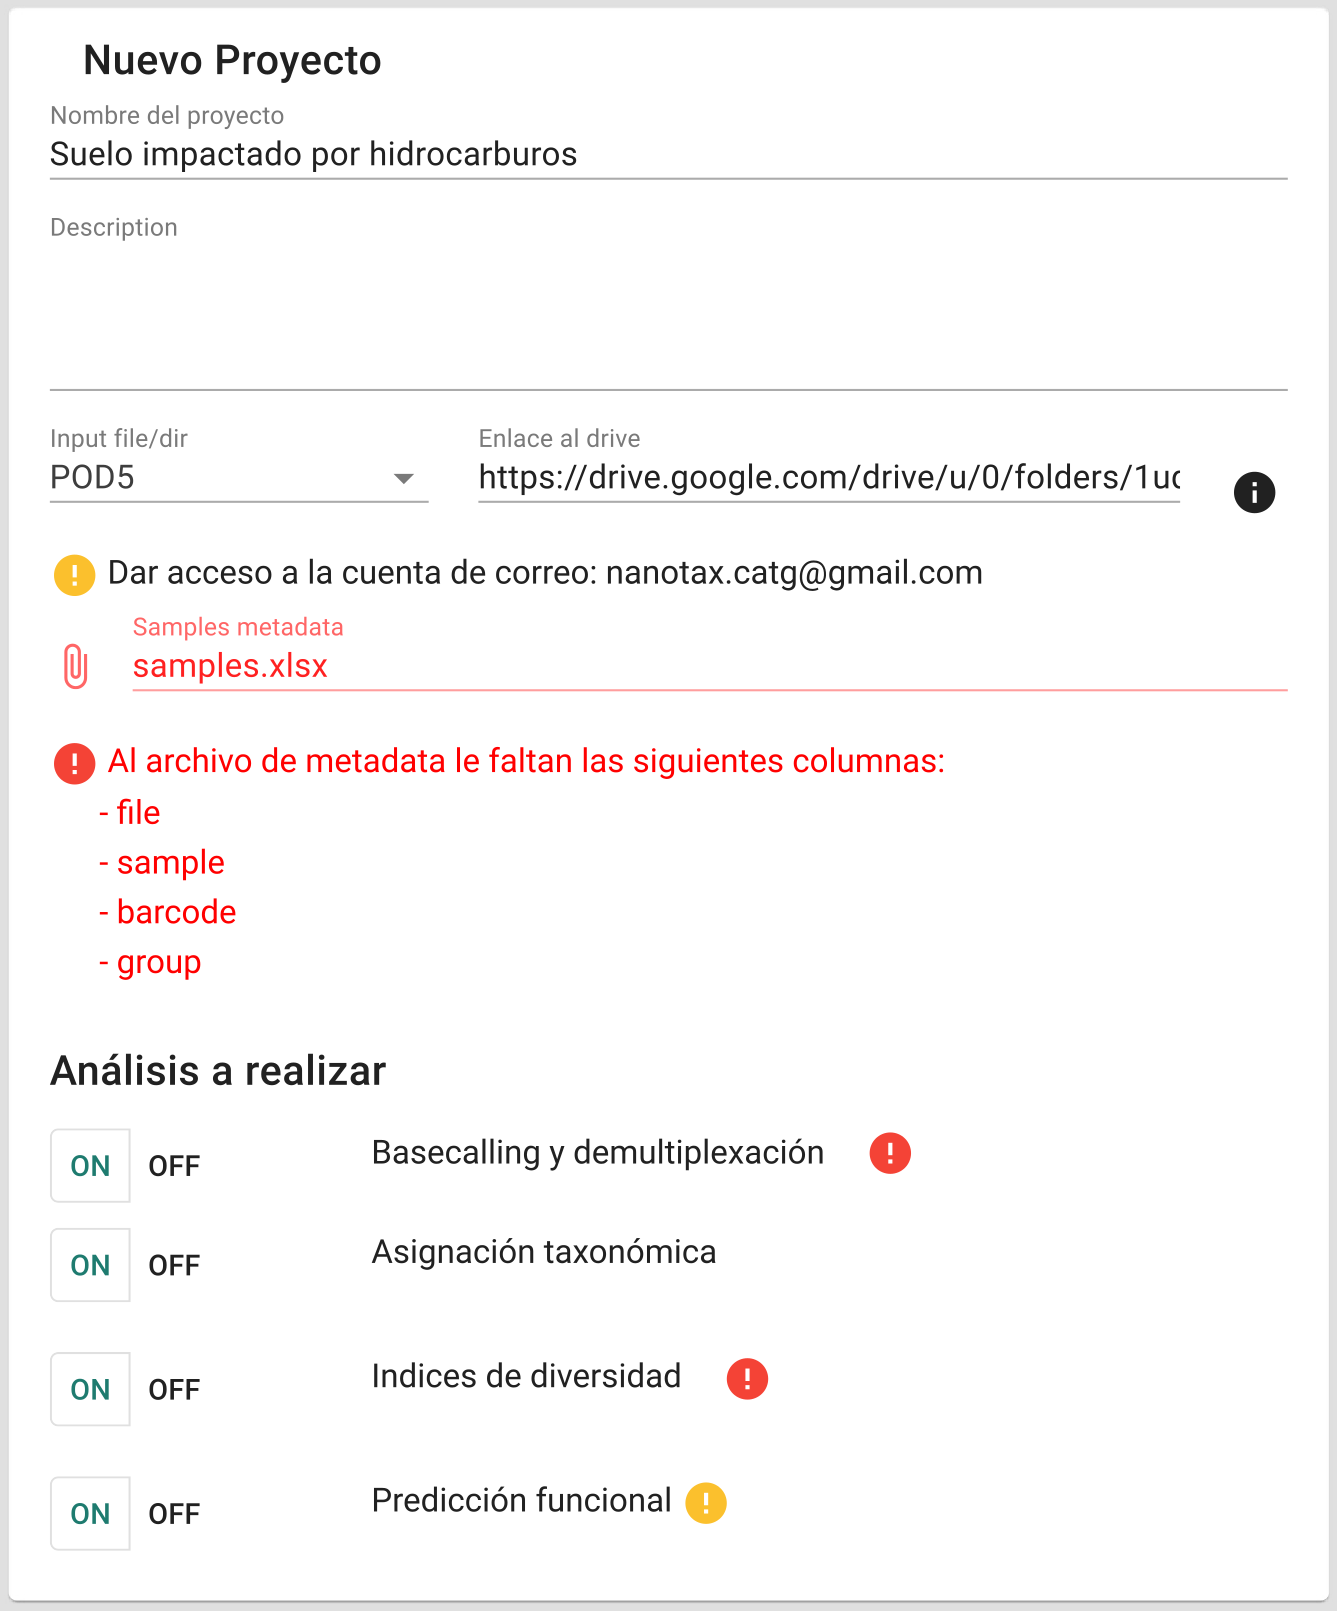
\includegraphics[width=\textwidth]{images/app/newAnalysis/metadata-error-1.png}
%         \caption{Vista de nuevo análisis: Errores en el archivo de metadata}
%         \label{fig:app-new-analysis-metadata-error}
%     \end{subfigure}
%     \caption{Vista de nuevo análisis: Errores }
%     \label{fig:app-new-analysis-metadata-nodata-error}
% \end{figure}



% En la parte inferior del componente se encuentra el botón de Subir data, el cual al hacer click en el, ingresará la información a la base de datos y copiará los archivos a la plataforma de computo. Una vez que el usuario presionar el botón de subir data, la plataforma se encarga de verificar que se cuente con toda la información necesaria para correr el pipeline.





% %%%%%%%%%%%%%%%%%%%%%%%%%%%%%%%%%%%%%%%%%%%%%%%%%%%%%%%%%%%%%%%%%%%%%%

% \subsection{Resultados/Proyectos} \label{projects}
% Una vez que el usuario valida sus credenciales en la plataforma será redireccionado a la sección de Resultados. En esta sección se mostraran los proyectos que el usuario ha subido a la plataforma, estos proyectos pueden estar en ejecución, finalizados o finalizados con errores. 
% Por cada proyecto se desplegará la información básica en una tarjeta:
% \begin{itemize}
%     \item Nombre del proyecto
%     \item Descripción del proyecto
%     \item Cantidad de muestras procesadas, descartadas y totales
%     \item Estado del proyecto (corriendo, finalizado, subido con errores)
%     \item En caso de que el proyecto haya finalizado el usuario podrá acceder a la sección especifica de resultados del proyecto mediante el botón de Ver resultados.
% \end{itemize}

% A continuación se presenta un ejemplo de la vista de proyectos subidos a la plataforma (Figura~\ref{fig:app-results-projects}).
% El primer proyecto se encuentra \textit{corriendo} por lo que no se tiene acceso a los resultados (botón de de ver resultados) ni a la información de las muestras descartadas ni analizadas correctamente.
% El segundo proyecto se encuentra finalizado, por lo que se puede acceder a los resultados y se puede visualizar además la cantidad de muestras procesadas, descartadas y totales. 

% \begin{figure}[H]
%     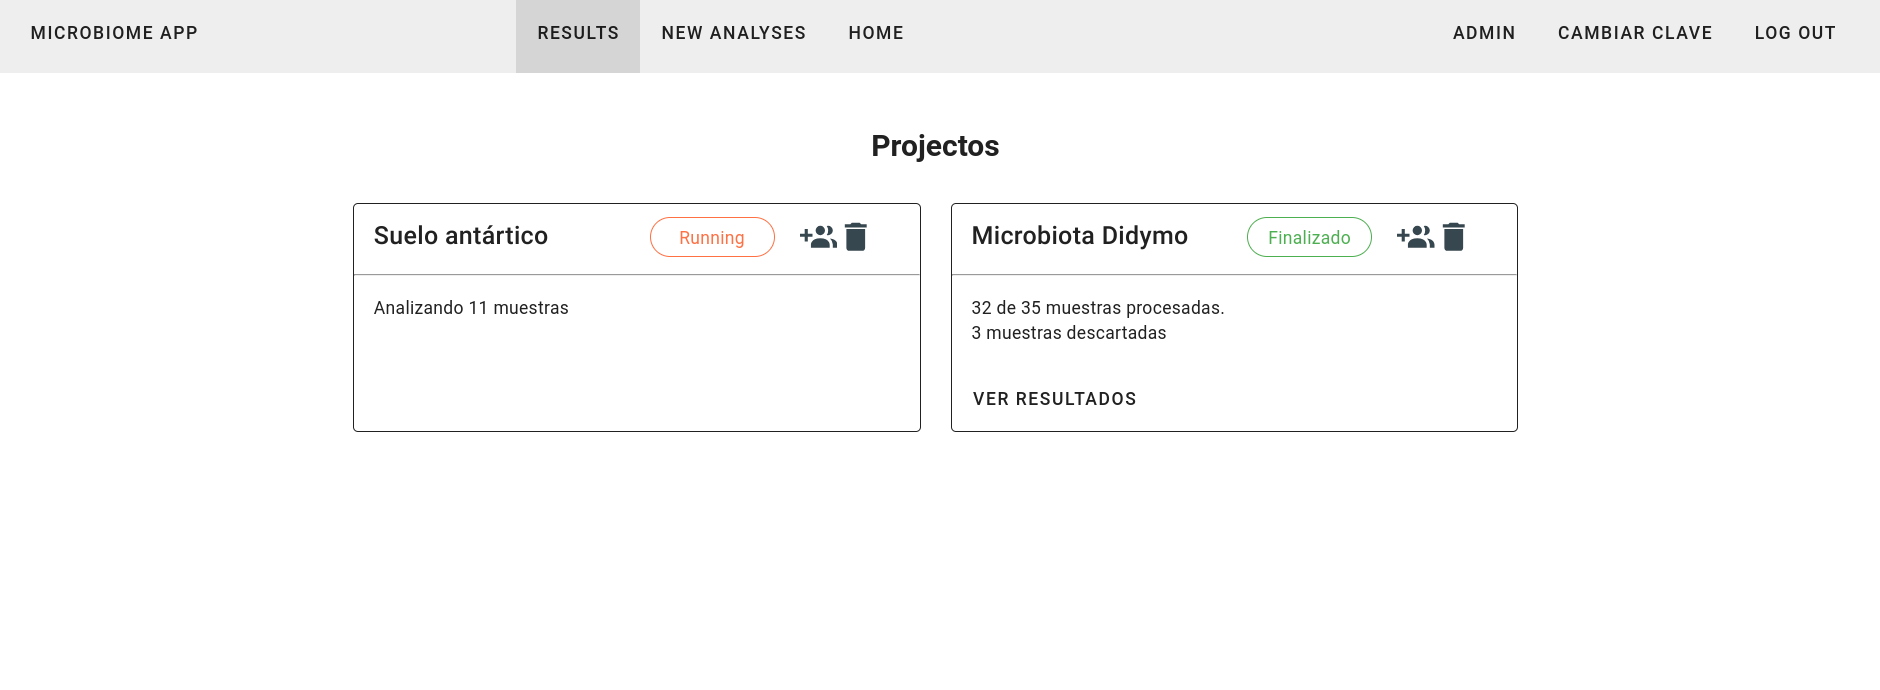
\includegraphics[width=1\linewidth]{images/app/projects.png}
%     % \captionsetup{justification=raggedright, width=0.45\linewidth, singlelinecheck=off}

%     % \captionsetup{width=0.45\linewidth}
%     \caption{Vista de proyectos subidos a la plataforma}
%     \label{fig:app-results-projects}
% \end{figure}
% En la parte superior de la tarjeta del proyecto se pueden visualizar dos íconos, uno para eliminar el proyecto y otro para poder compartir los resultados del proyecto con otros usuarios de la plataforma.


% En el caso de seleccionar el botón para añadir usuarios se desplegará una ventana emergente donde se podrá ingresar el nombre de usuario al que se desea compartir los resultados del proyecto(Figura~\ref{fig:app-add-project}). 
% En caso de que el usuario no exista en la plataforma se mostrará un mensaje de error \textit{“Usuario no encontrado”} (Figura~\ref{fig:app-add-project-invalid-usar}).
% \begin{figure}[H]
%         \centering
%         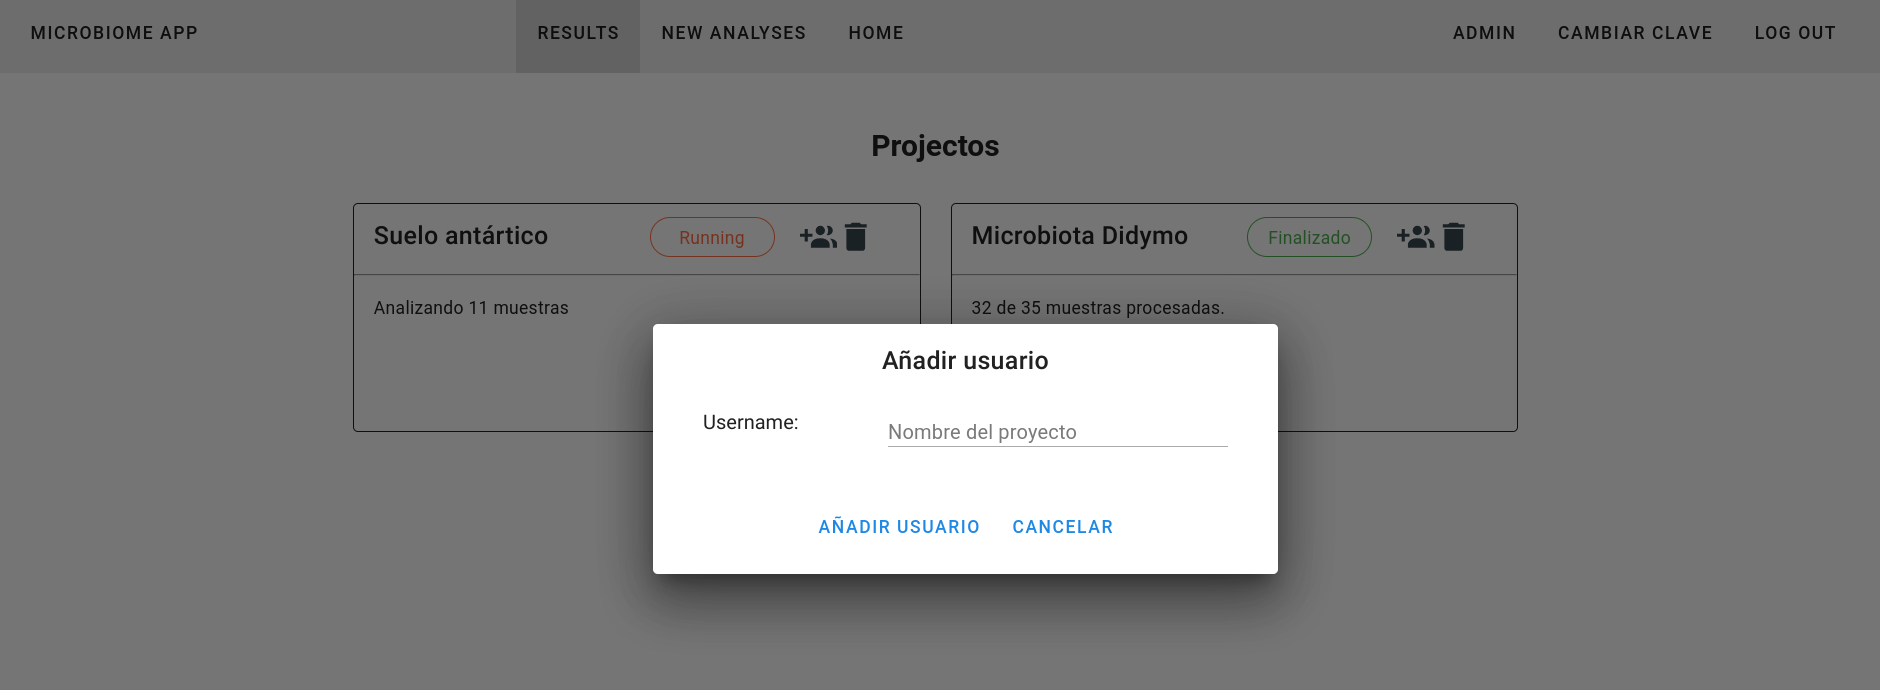
\includegraphics[width=\textwidth]{images/app/addUser.png}
%         \caption{Añadir usuario a un proyecto existente}
%         \label{fig:app-add-project}

% \end{figure}

% \begin{figure}[H]
%     \centering
%     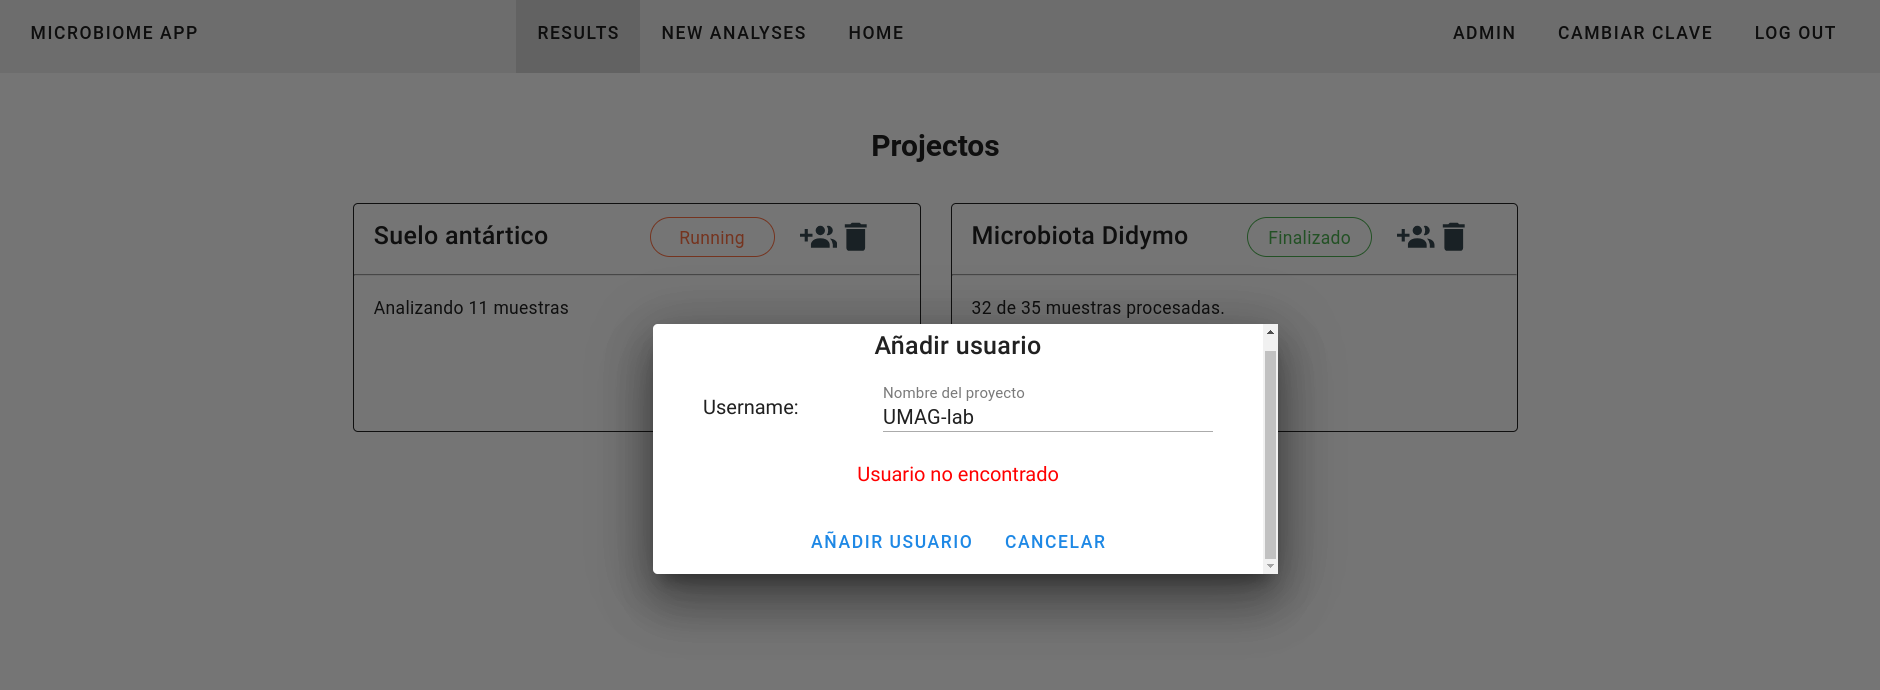
\includegraphics[width=\textwidth]{images/app/addUser_notFound.png}
%     \caption{Añadir usuario a un proyecto existente: Mensaje de error debido a que el usuario no existe en la plataforma}
%     \label{fig:app-add-project-invalid-usar}

% \end{figure}

% En el caso de seleccionar el icono para eliminar el proyecto se desplegará una ventana emergente con un mensaje de confirmación, en caso de confirmar la eliminación del proyecto se eliminará toda la información asociada al proyecto de la base de datos y se eliminarán los archivos asociados al proyecto de la plataforma de computo~\ref{fig:app-delete-project}.

% \begin{figure}[H]
%     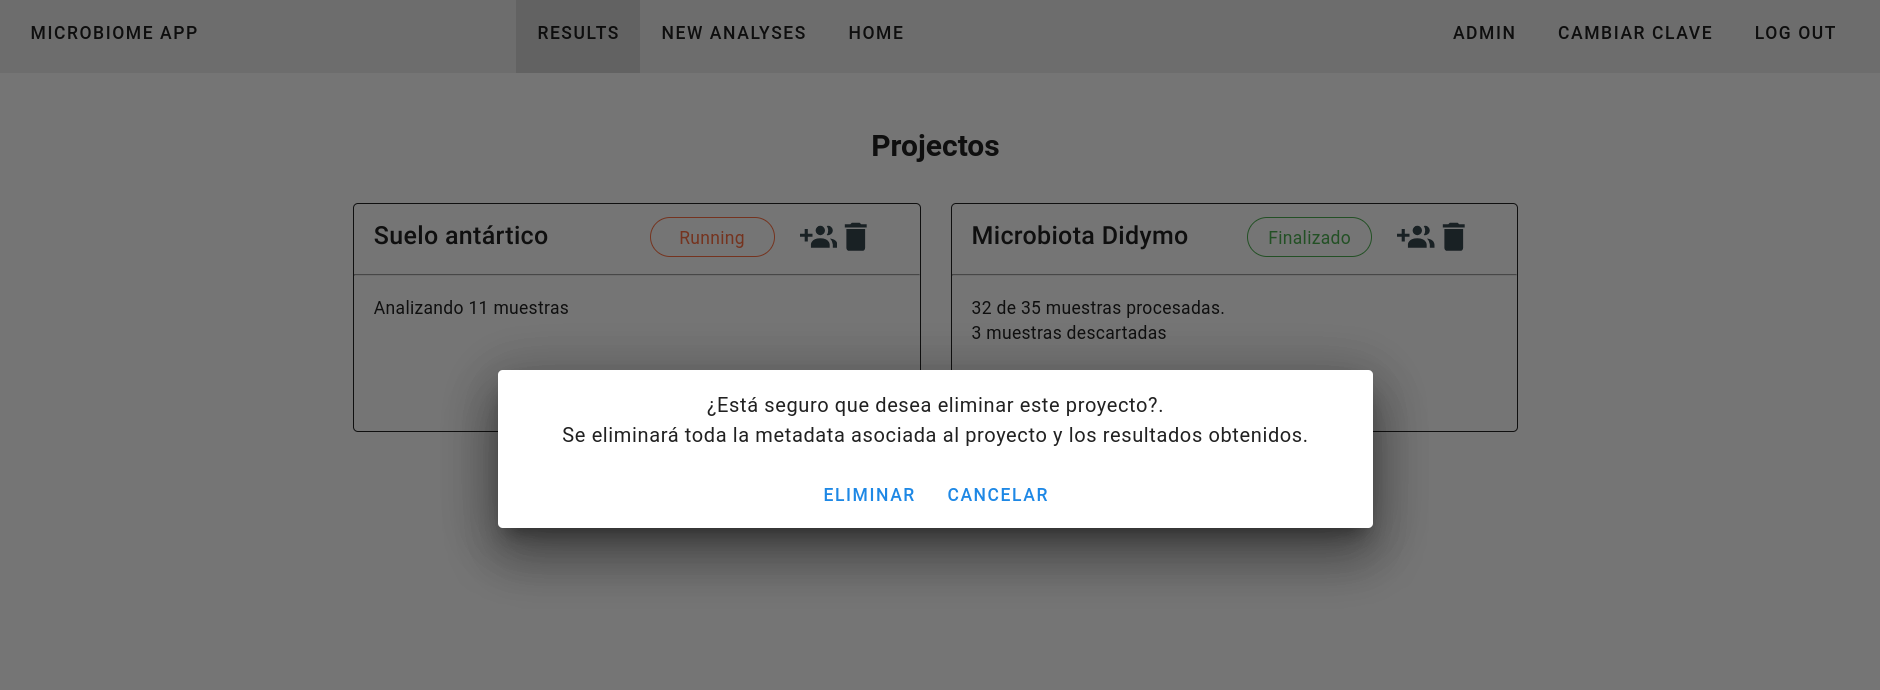
\includegraphics[width=1\linewidth]{images/app/deleteProject.png}
%     % \captionsetup{justification=raggedright, width=0.45\linewidth, singlelinecheck=off}

%     % \captionsetup{width=0.45\linewidth}
%     \caption{Eliminar proyecto de la plataforma}
%     \label{fig:app-delete-project}
% \end{figure}

% \subsection{Resultados de un proyecto en especifico}
% Una vez que el pipeline haya finalizado su ejecución, la plataforma permitirá al usuario acceder a los resultados de cada proyecto leyendo los resultados desde la base de datos y desplegando la información en la sección de resultados de cada proyecto.
% Esta sección cuenta con 5 subsecciones, cada una con información específica del análisis realizado. 
% En caso de que al ingresar el proyecto el usuario no seleccione todos los análisis, solo se mostrarán las secciones indicadas por el usuario.

% \subsection{Información básica de las muestras}
% %Esta sección se mostrará siempre que el usuario empiece con archivos POD5 o FastQ, es decir, ya sea comenzando el análisis desde el basecalling o desde el control de calidad. \hl{Igual si es que solo se hace asignaicón taxonomica}.
% Esta sección se desplegará siempre en la plataforma y cuenta en el lado izquierdo con una tabla con información básica de las muestras y en el lado derecho un gráfico que representa la calidad y tamaño promedio de las lecturas.
% La tabla esta compuesta por los siguientes elementos:
% \begin{itemize}
%     \item Nombre de la muestra: Nombre indicado en el archivo de metadata al ingresar el proyecto.
%     % \item \hl{Grupo}: Grupo asociado a la muestra en el archivo de metadata (en caso de ingresar grupo).
%     \item Total de lecturas: Cantidad de lecturas previo a los filtros de calidad.
%     \item Calidad promedio: Calidad promedio en formato phred despues de los filtros de calidad.
%     \item Largo promedio: Largo promdio despues de los filtros de calidad
%     \item Lecturas después de los filtros: Cantidad de lecturas luego de los filtros de calidad.
%     \item Nota: Si la muestra fue descartada por no contar con la cantidad suficiente de lecturas se informará en esta columna.
% \end{itemize}
% En la parte inferior de la tabla hay una nota que indica la cantidad de lecturas que se consideraron para los análisis posteriores, este valor por defecto es 100.000, pudiendo ser modificado por el usuario en las opciones avanzadas al ingresar el proyecto.

% En la parte derecha de la sección se puede visualizar un heatmap donde en el eje X se encuentra el tamaño de las secuencias, y en el eje Y la calidad. 
% El color indica la cantidad de lecturas que se encuentran en esa intersección, mientras más intenso el color, más secuencias tienen la calidad y tamaño indicado.
% Para este grafico se consideraron todas las muestras con sus lecturas después de los filtros de calidad.

% % En la parte inferior del gráfico hay una nota que indica en que rangos de tamaño se encuentran la mayoria de las lecturas\hl{Muy generico?}. 
% A continuación se presenta un ejemplo de la sección de información básica de las muestras (Figura~\ref{fig:app-results-basicStatistics}).
% \begin{figure}[H]
%     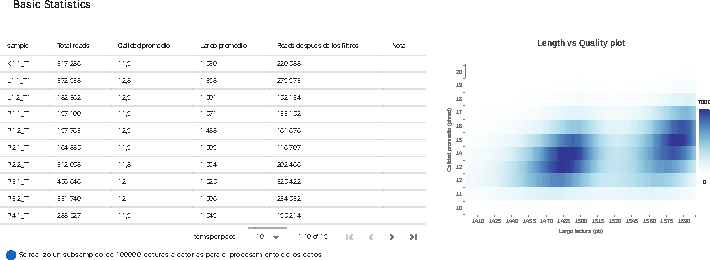
\includegraphics[width=1\linewidth]{images/app/results/basicStatistics.pdf}
%     % \captionsetup{justification=raggedright, width=0.45\linewidth, singlelinecheck=off}

%     % \captionsetup{width=0.45\linewidth}
%     \caption{Estadisticas básicas (resultados)}
%     \label{fig:app-results-basicStatistics}
% \end{figure}

% En caso de que el usuario ingrese un valor mínimo de lecturas para realizar los análisis y alguna de las muestras no cumpla con este valor, se mostrará un mensaje de error en la tabla de información básica de las muestras (Figura~\ref{fig:app-results-basicStatistics-exclude}).
% \begin{figure}[H]
%     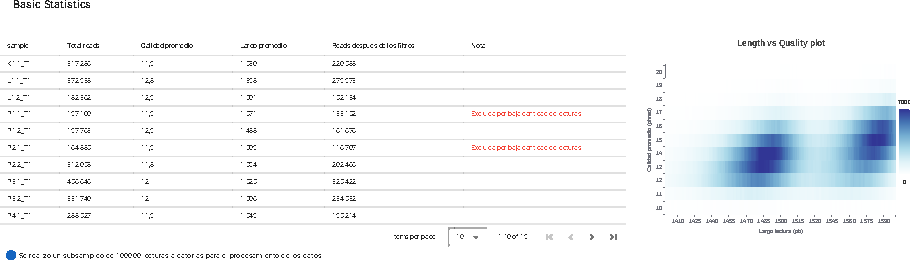
\includegraphics[width=1\linewidth]{images/app/results/basicStatistics_exclude.pdf}
%     % \captionsetup{justification=raggedright, width=0.45\linewidth, singlelinecheck=off}

%     % \captionsetup{width=0.45\linewidth}
%     \caption{Estadisticas básicas (resultados)}
%     \label{fig:app-results-basicStatistics-exclude}
% \end{figure}

% \subsection{Asignación taxonómica}
% En la parte superior de esta sección se pueden visualizar pestañas que representan cada categoría taxonómica (especie, género, familia, orden, clase y filo), las cuales permiten ajustar la visualización de la información presentada en esta  sección (gráfico de barras apiladas y tabla). Por defecto se presenta la información para la categoría de especie.

% Debajo de las pestañas en el lado izquierdo hay un gráfico de barras apiladas que permite visualizar la abundancia de las taxonomías en cada muestra.
% El usuario puede interactuar con el gráfico modificando la visualización a través de los botones que se encuentran en la parte inferior, pudiendo visualizar la información en porcentaje o en cantidad de lecturas, como también pudiendo modificar el porcentaje mínimo para crear la categoria \textit{Otros}.
% En caso de que el usuario hubiera ingresado información de grupos asociados a las muestras, se podrá visualizar un nuevo grupo de botones que permite al usuario visualizar la información de las taxonomías por grupo o por muestra.
% La leyenda del gráfico de barras apiladas presenta solo las 10 taxonomías con mayor abundancia. 
% Por defecto, todas aquellas taxonomías que tengan un valor menor al 0.01\% de abundancia serán eliminadas y aquellas con un porcentaje menor a un 1\%  serán agrupadas en una nueva taxonomia llamada \textit{Otros}.


% A continuación se puede visualizar como se presenta la sección de taxonomía en la plataforma (Figura~\ref{fig:app-results-taxonomy}).

% \begin{figure}[H]
%     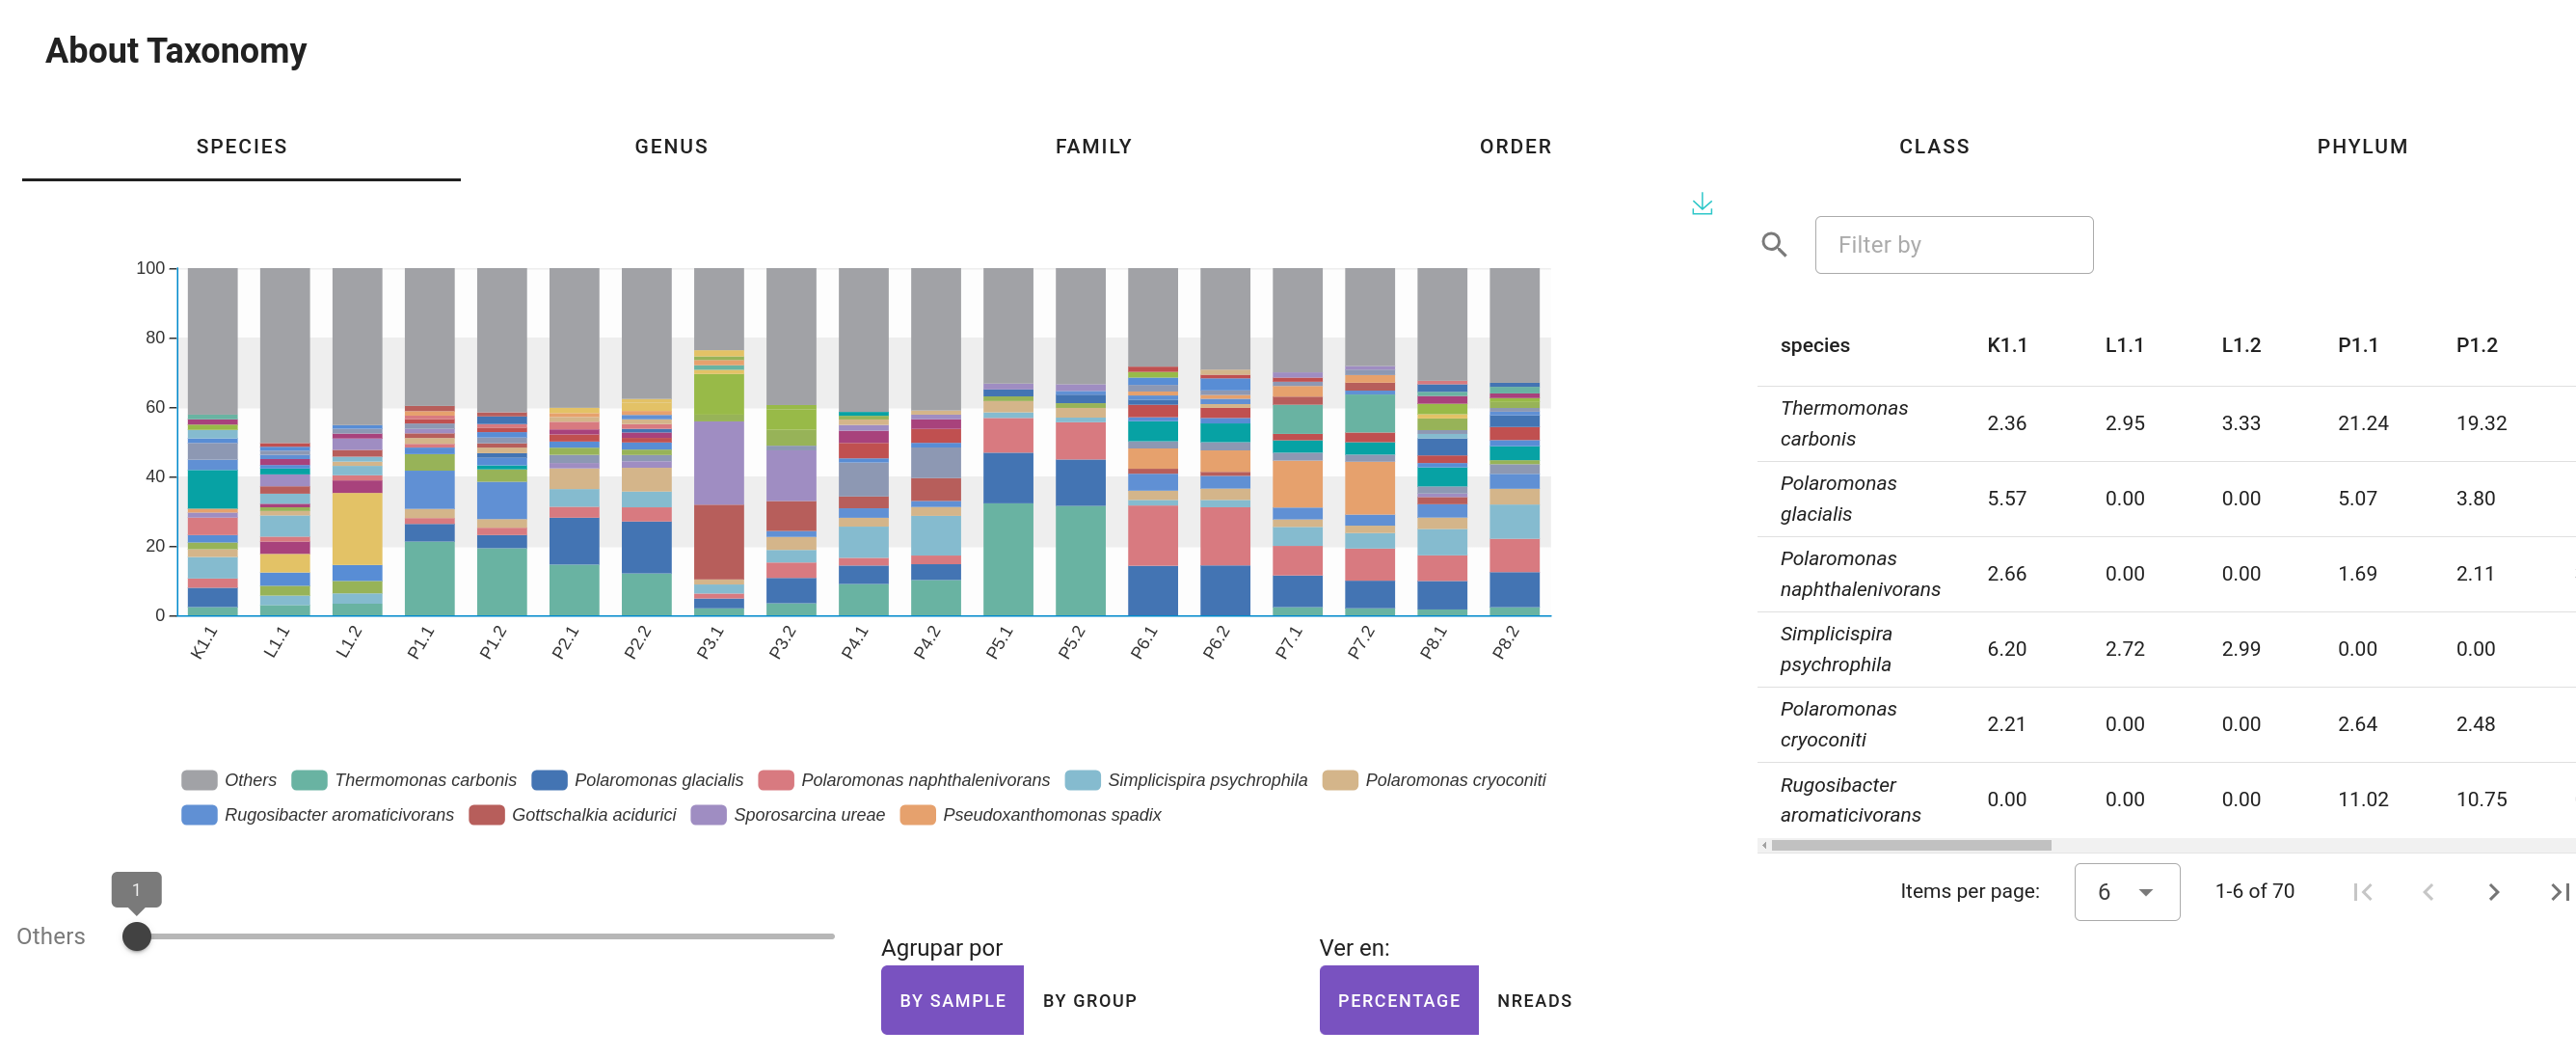
\includegraphics[width=1\linewidth]{images/app/results/taxonomy.png}
%     % \captionsetup{justification=raggedright, width=0.45\linewidth, singlelinecheck=off}

%     % \captionsetup{width=0.45\linewidth}
%     \caption{Vista de asignación taxonómica (resultados)}
%     \label{fig:app-results-taxonomy}
% \end{figure}

% % En el lado derecho, hay una tabla que permite visualizar el detalle de la información presentada en el gráfico. 
% % Se puede visualizar además un campo de texto que permite al usuario buscar una taxonomía en especifico y visualizar su abundancia o cantidad de lecturas en todas las muestras.

% En caso de que la pantalla tenga una resolución menor a 992px la tabla y gráfico se desplegarán uno debajo del otro(Figura~\ref{fig:app-results-taxonomy-small-dev}).
% \begin{figure}[H]
%     \centering
%     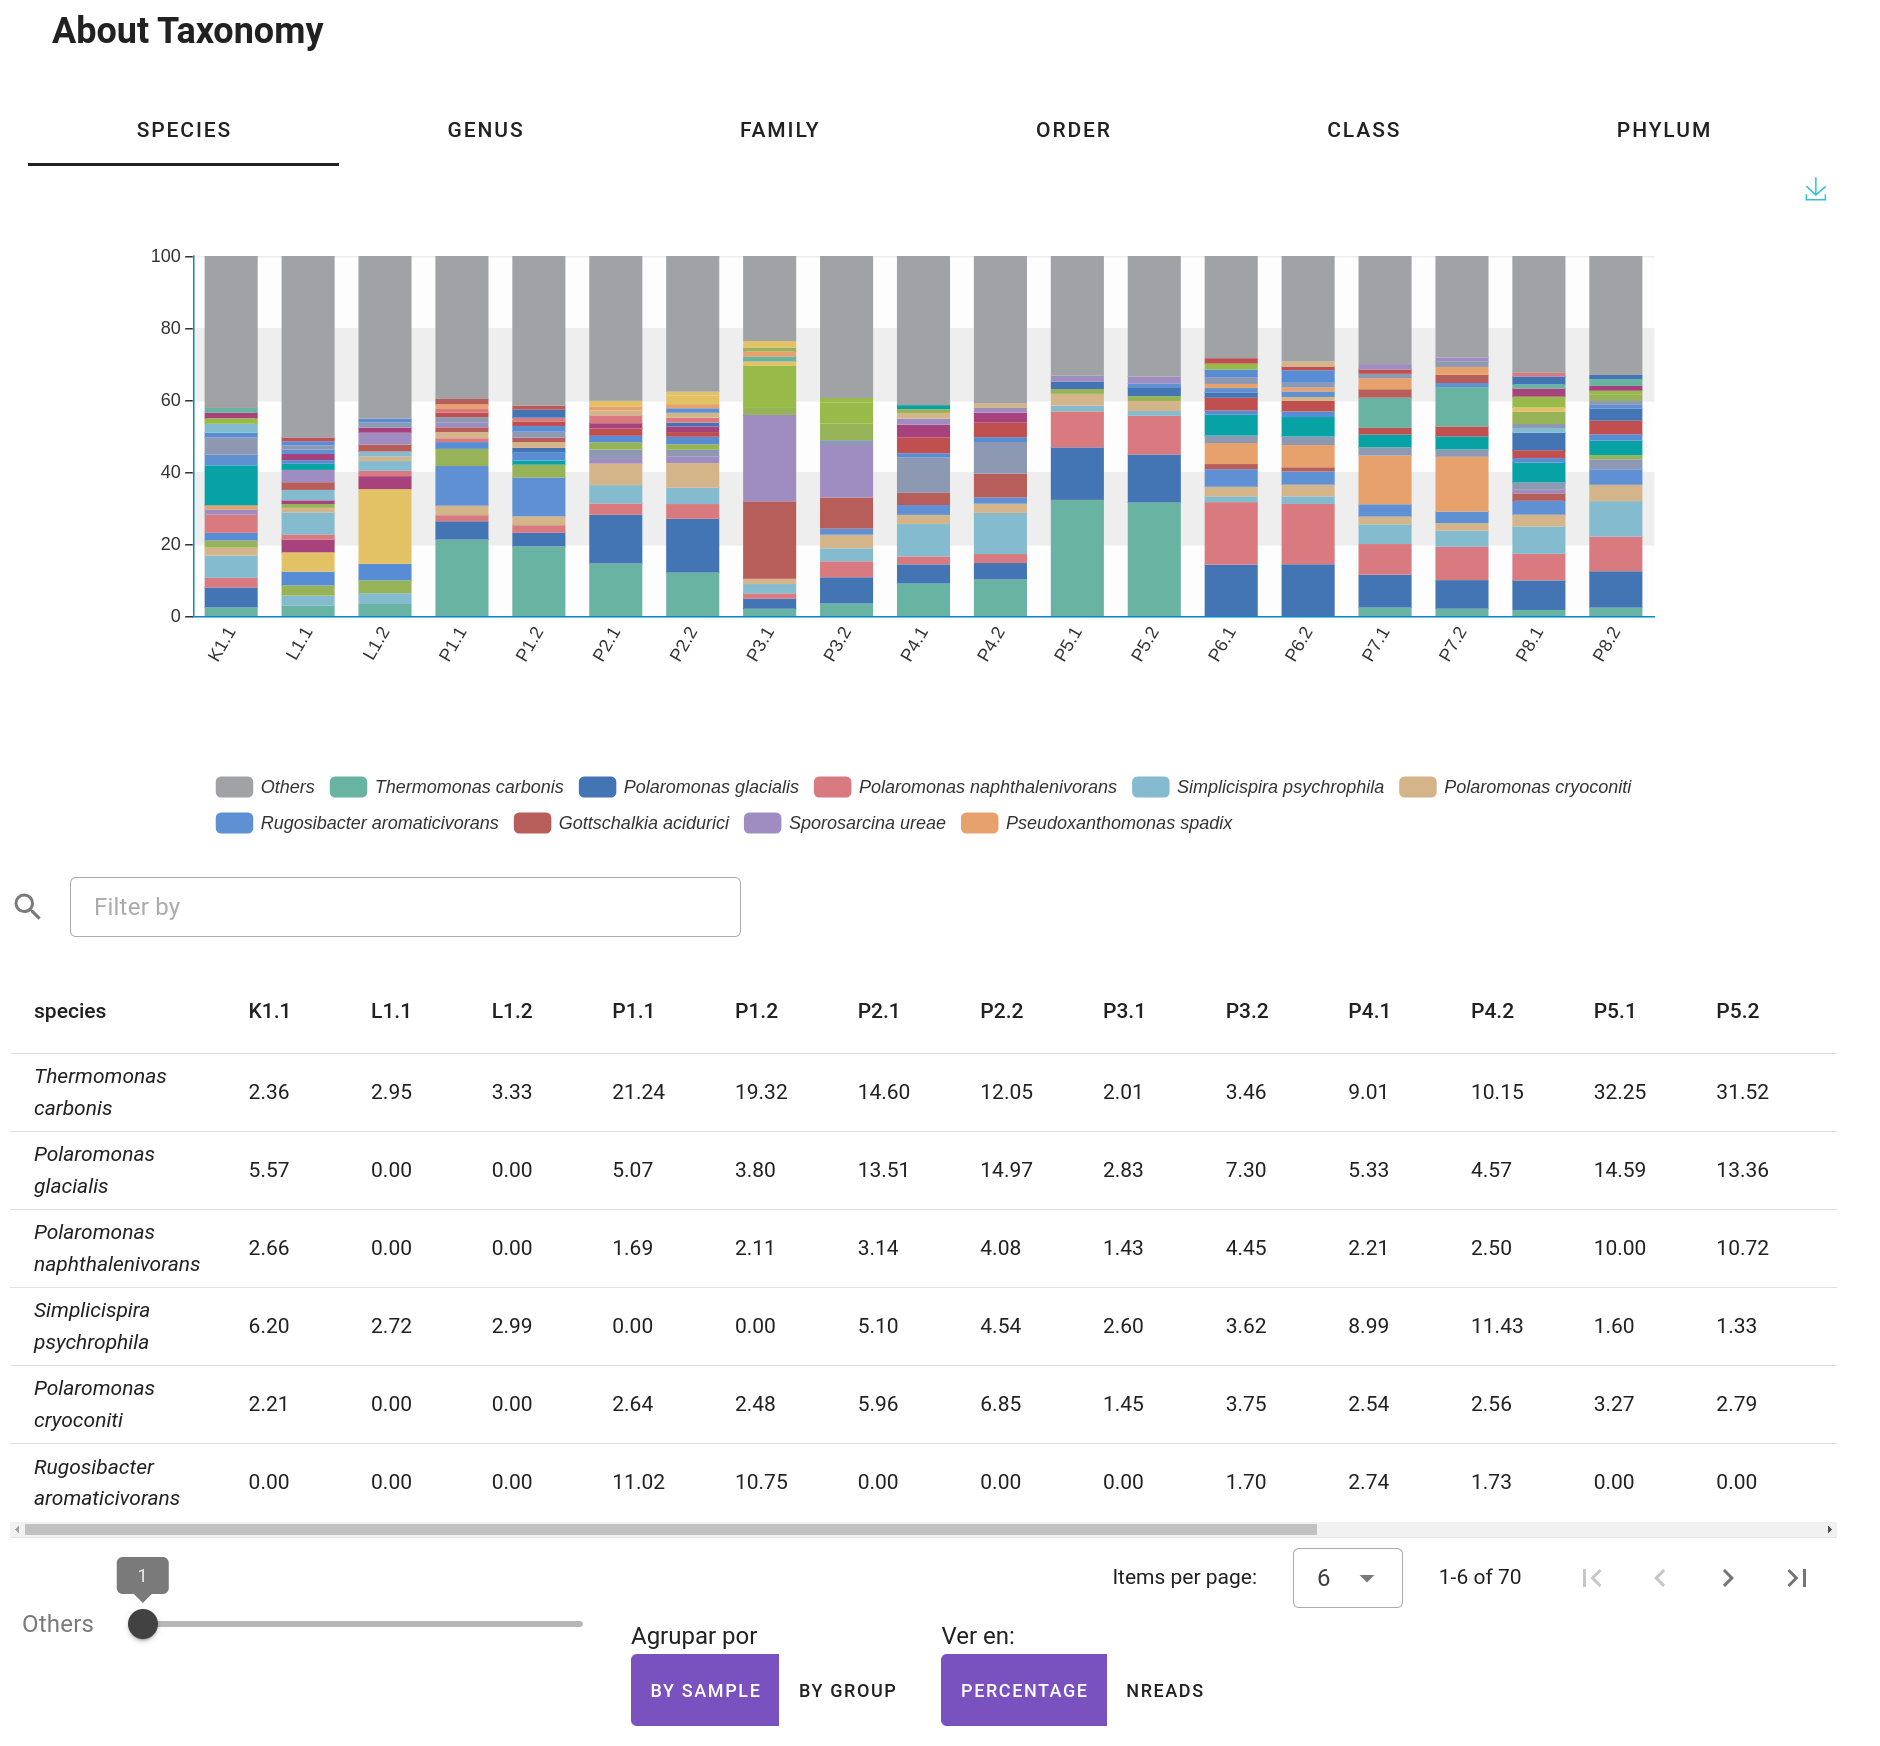
\includegraphics[width=0.8\linewidth]{images/app/results/taxonomy_small_dev.png}
%     % \captionsetup{justification=raggedright, width=0.45\linewidth, singlelinecheck=off}

%     % \captionsetup{width=0.45\linewidth}
%     \caption{Estadisticas básicas (resultados)}
%     \label{fig:app-results-taxonomy-small-dev}
% \end{figure}

% Ambos componentes, la tabla y el gráfico de barras apiladas se ajustan automáticamente para presentar la información requerida por el usuario, es decir, cada vez que el usuario selecciona una nueva categoría taxonómica en las pestañas, se vuelve a generar la información proporcionando una visualización clara y detallada de los datos.







% % El usuario puede modificar la visualización de la información en el gráfico de barras apiladas y tabla a través de las pestañas que se encuentran en la parte superior del gráfico 
% En la Figura~\ref{fig:app-results-taxonomy-order} el usuario seleccionó la pestaña de orden, por lo que se visualiza la información de la taxonomía en la categoría de orden.
% \begin{figure}[H]
%     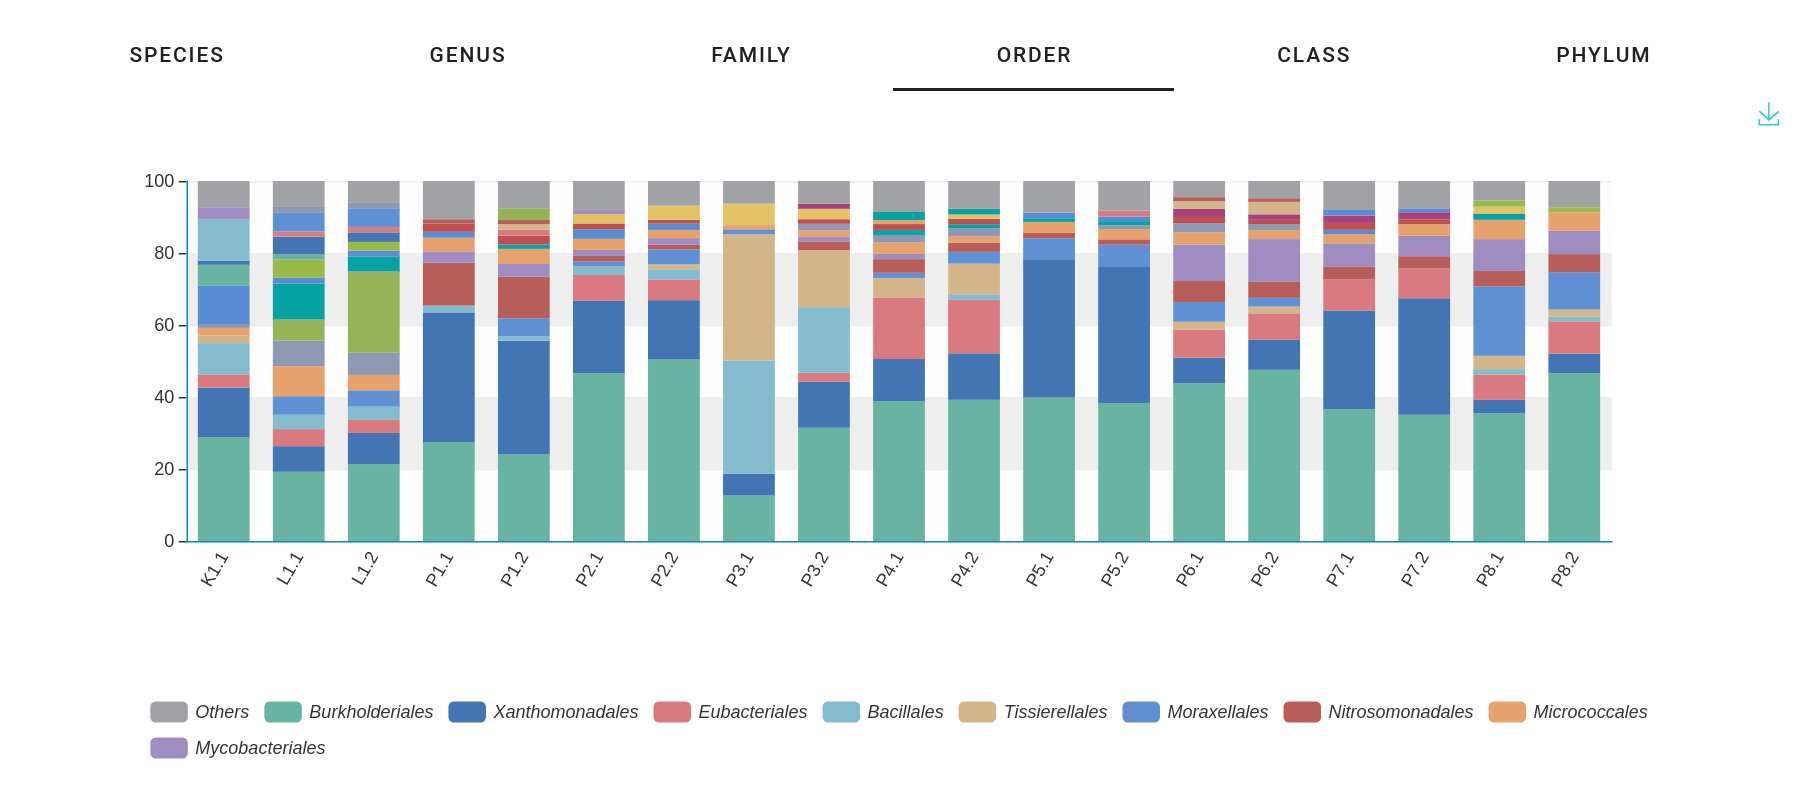
\includegraphics[width=1\linewidth]{images/app/results/taxonomy_order.png}
%     % \captionsetup{justification=raggedright, width=0.45\linewidth, singlelinecheck=off}

%     % \captionsetup{width=0.45\linewidth}
%     \caption{Vista de asignación taxonómica en categoría de orden (stacked plot)}
%     \label{fig:app-results-taxonomy-order}
% \end{figure}



% % \begin{figure}[H]
% %     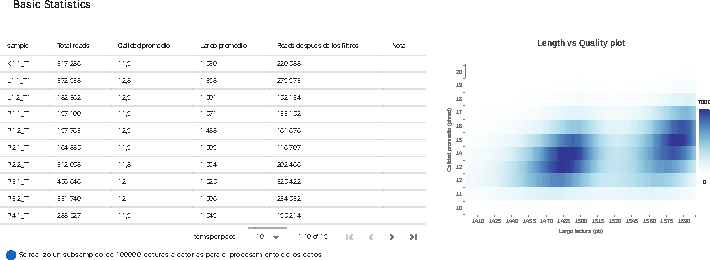
\includegraphics[width=1\linewidth]{images/app/results/basicStatistics.png}
% %     % \captionsetup{justification=raggedright, width=0.45\linewidth, singlelinecheck=off}

% %     % \captionsetup{width=0.45\linewidth}
% %     \caption{Estadisticas básicas (resultados)}
% %     \label{fig:app-results-taxonomicAssig-group-perc}
% % \end{figure}




% El usuario también puede modificar la información de la tabla y gráfico utilizando los botones que se encuentran en la parte inferior del gráfico. 
% Pudiendo visualizar la información en porcentaje o en cantidad de lecturas~\ref{fig:app-results-taxonomy-sample-nreads}, como también pudiendo agrupar las muestras por grupo~\ref{fig:app-results-taxonomy-groups-perc}.
% \begin{figure}[H]
%     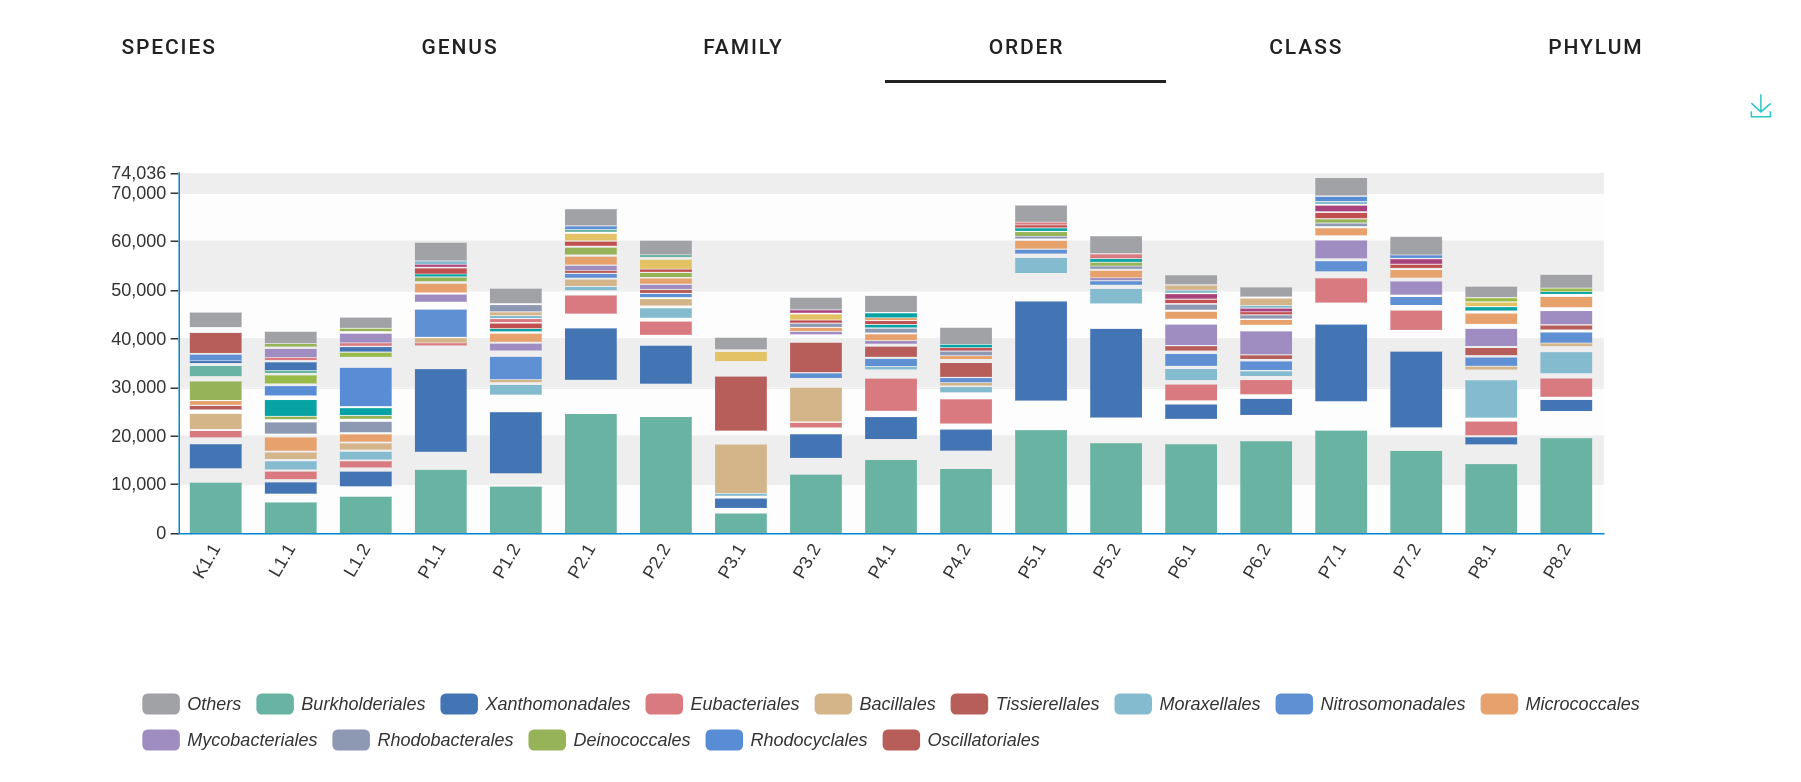
\includegraphics[width=1\linewidth]{images/app/results/taxonomy_sample_nreads.png}
%     % \captionsetup{justification=raggedright, width=0.45\linewidth, singlelinecheck=off}

%     % \captionsetup{width=0.45\linewidth}
%     \caption{Taxonomias por muestra utilizando cantidad de lecturas}
%     \label{fig:app-results-taxonomy-sample-nreads}
% \end{figure}

% \begin{figure}[H]
%     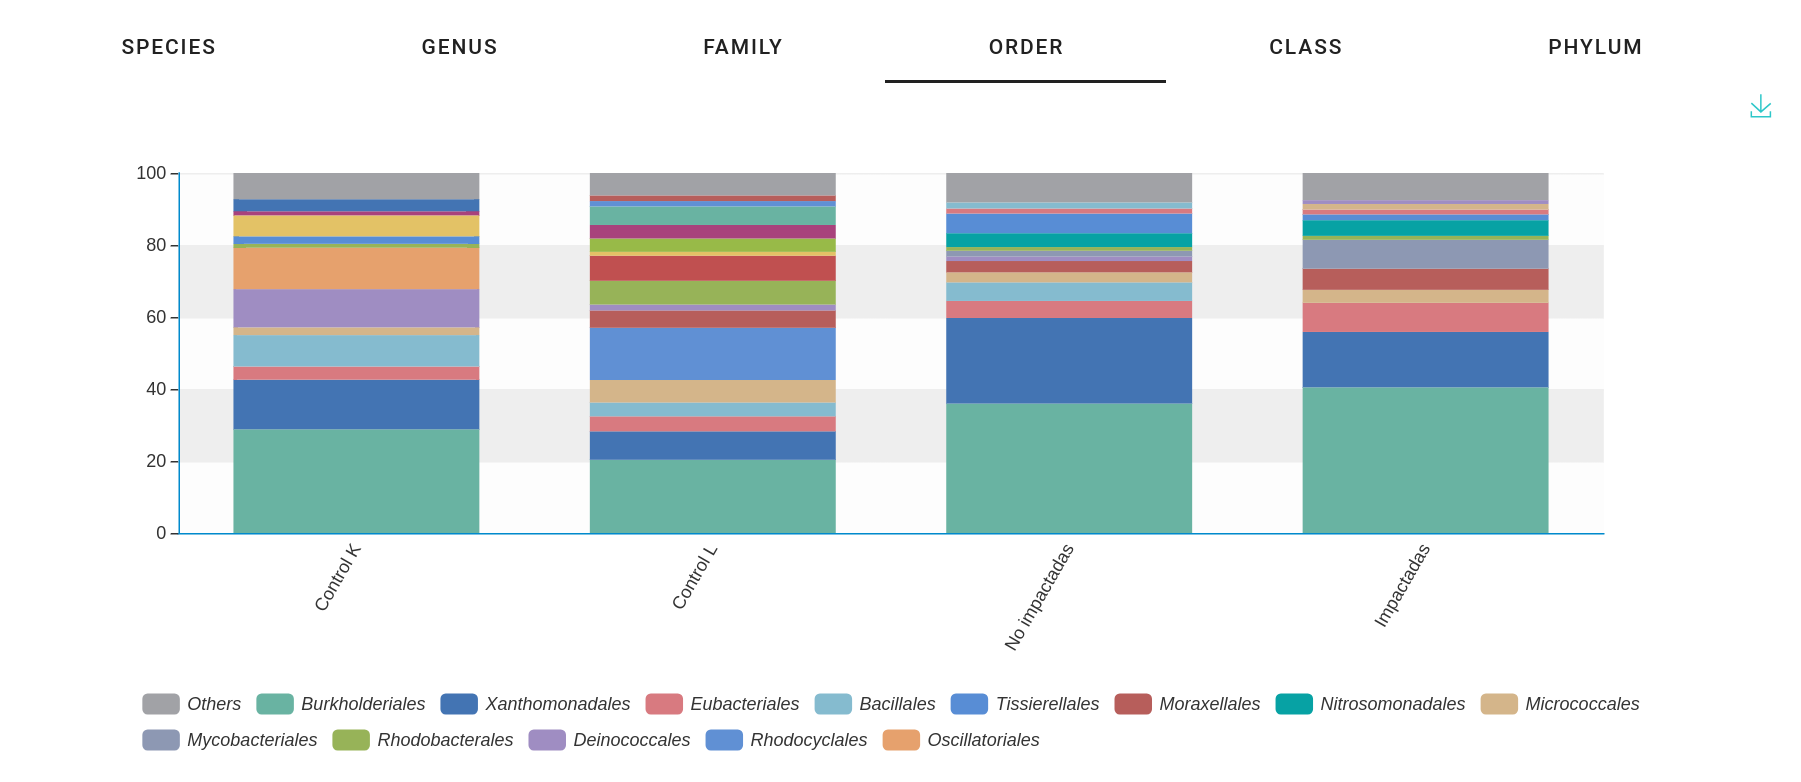
\includegraphics[width=1\linewidth]{images/app/results/taxonomy_grooups_perc.png}
%     % \captionsetup{justification=raggedright, width=0.45\linewidth, singlelinecheck=off}

%     % \captionsetup{width=0.45\linewidth}
%     \caption{Taxonomias por grupo utilizando valor porcentual}
%     \label{fig:app-results-taxonomy-groups-perc}
% \end{figure}


% De igual forma el usuario puede posicionar el mouse sobre alguna barra del gráfico o sobre alguna taxonomía de la leyenda y destacar esa taxonomía en todas las muestras y visualizar el porcentaje o cantidad de lecturas en la muestra que el mouse se encuentra posicionado (Figura~\ref{fig:app-results-taxonomicAssig-others}).
% \begin{figure}[H]
%     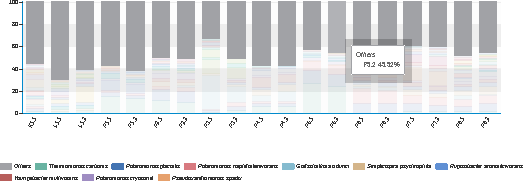
\includegraphics[width=1\linewidth]{images/app/results/taxonomy_others.pdf}
%     % \captionsetup{justification=raggedright, width=0.45\linewidth, singlelinecheck=off}

%     % \captionsetup{width=0.45\linewidth}
%     \caption{Taxonomía por muestra: Destacar taxonomía en todas las muestras}
%     \label{fig:app-results-taxonomicAssig-others}
% \end{figure}


% La tabla de taxonomías presenta un campo de búsqueda en la parte superior que permite al usuario filtrar la tabla por una taxonomía en especifico (Figura~\ref{fig:app-results-taxonomy-search}).
% En el ejemplo se busca la palabra \textit{Polar} por lo que aparecen todas taxonomías que contienen esta palabra en su nombre.
% \begin{figure}[H]
%     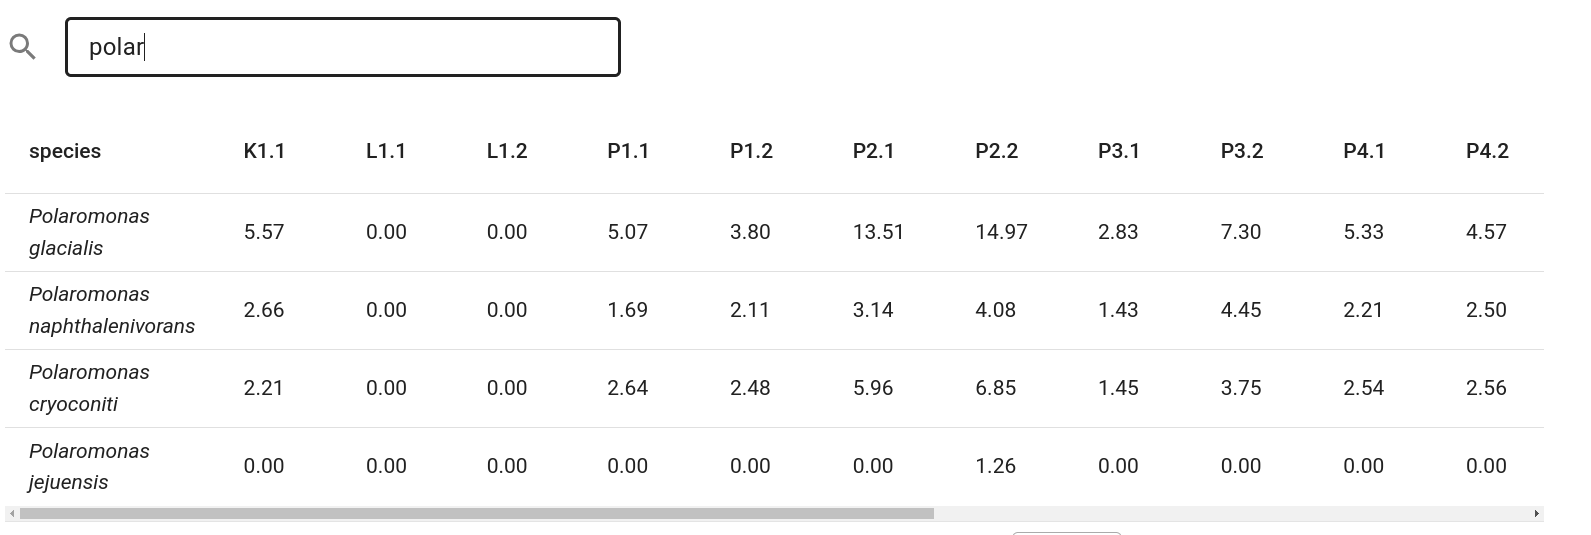
\includegraphics[width=0.9\linewidth]{images/app/results/taxonomy_search.png}
%     % \captionsetup{justification=raggedright, width=0.45\linewidth, singlelinecheck=off}

%     % \captionsetup{width=0.45\linewidth}
%     \caption{Filtro de resultados en tabla de asignación taxonómica}
%     \label{fig:app-results-taxonomy-search}
% \end{figure}

% \subsection{Similitud entre las muestras}
% Esta sección representa las taxonomías compartidas por las muestras mediante un gráfico circular de anillos jerarquicos. 
% Cada nivel del gráfico representa una categoría taxonómica, siendo la más interna especie, y la más externa filo.
% Mientras más grande el diamentro del anillo en el gráfico, mayor es la presencia de esa taxonomía en las muestras.

% Las taxonomías presentadas incluyen todas las taxonomías con abundancia mayor al 1\% y que estan presentes en todas las muestras del grupo.
% El porcentaje presentado corresponde el porcentaje de todas las lecturas en el grupo graficado.


% A continuación se presenta un ejemplo de como se visualiza el gráfico circular de anillos jerarquicos para dos grupos(Figura~\ref{fig:app-results-core}).
% \begin{figure}[H]
%     \centering
%     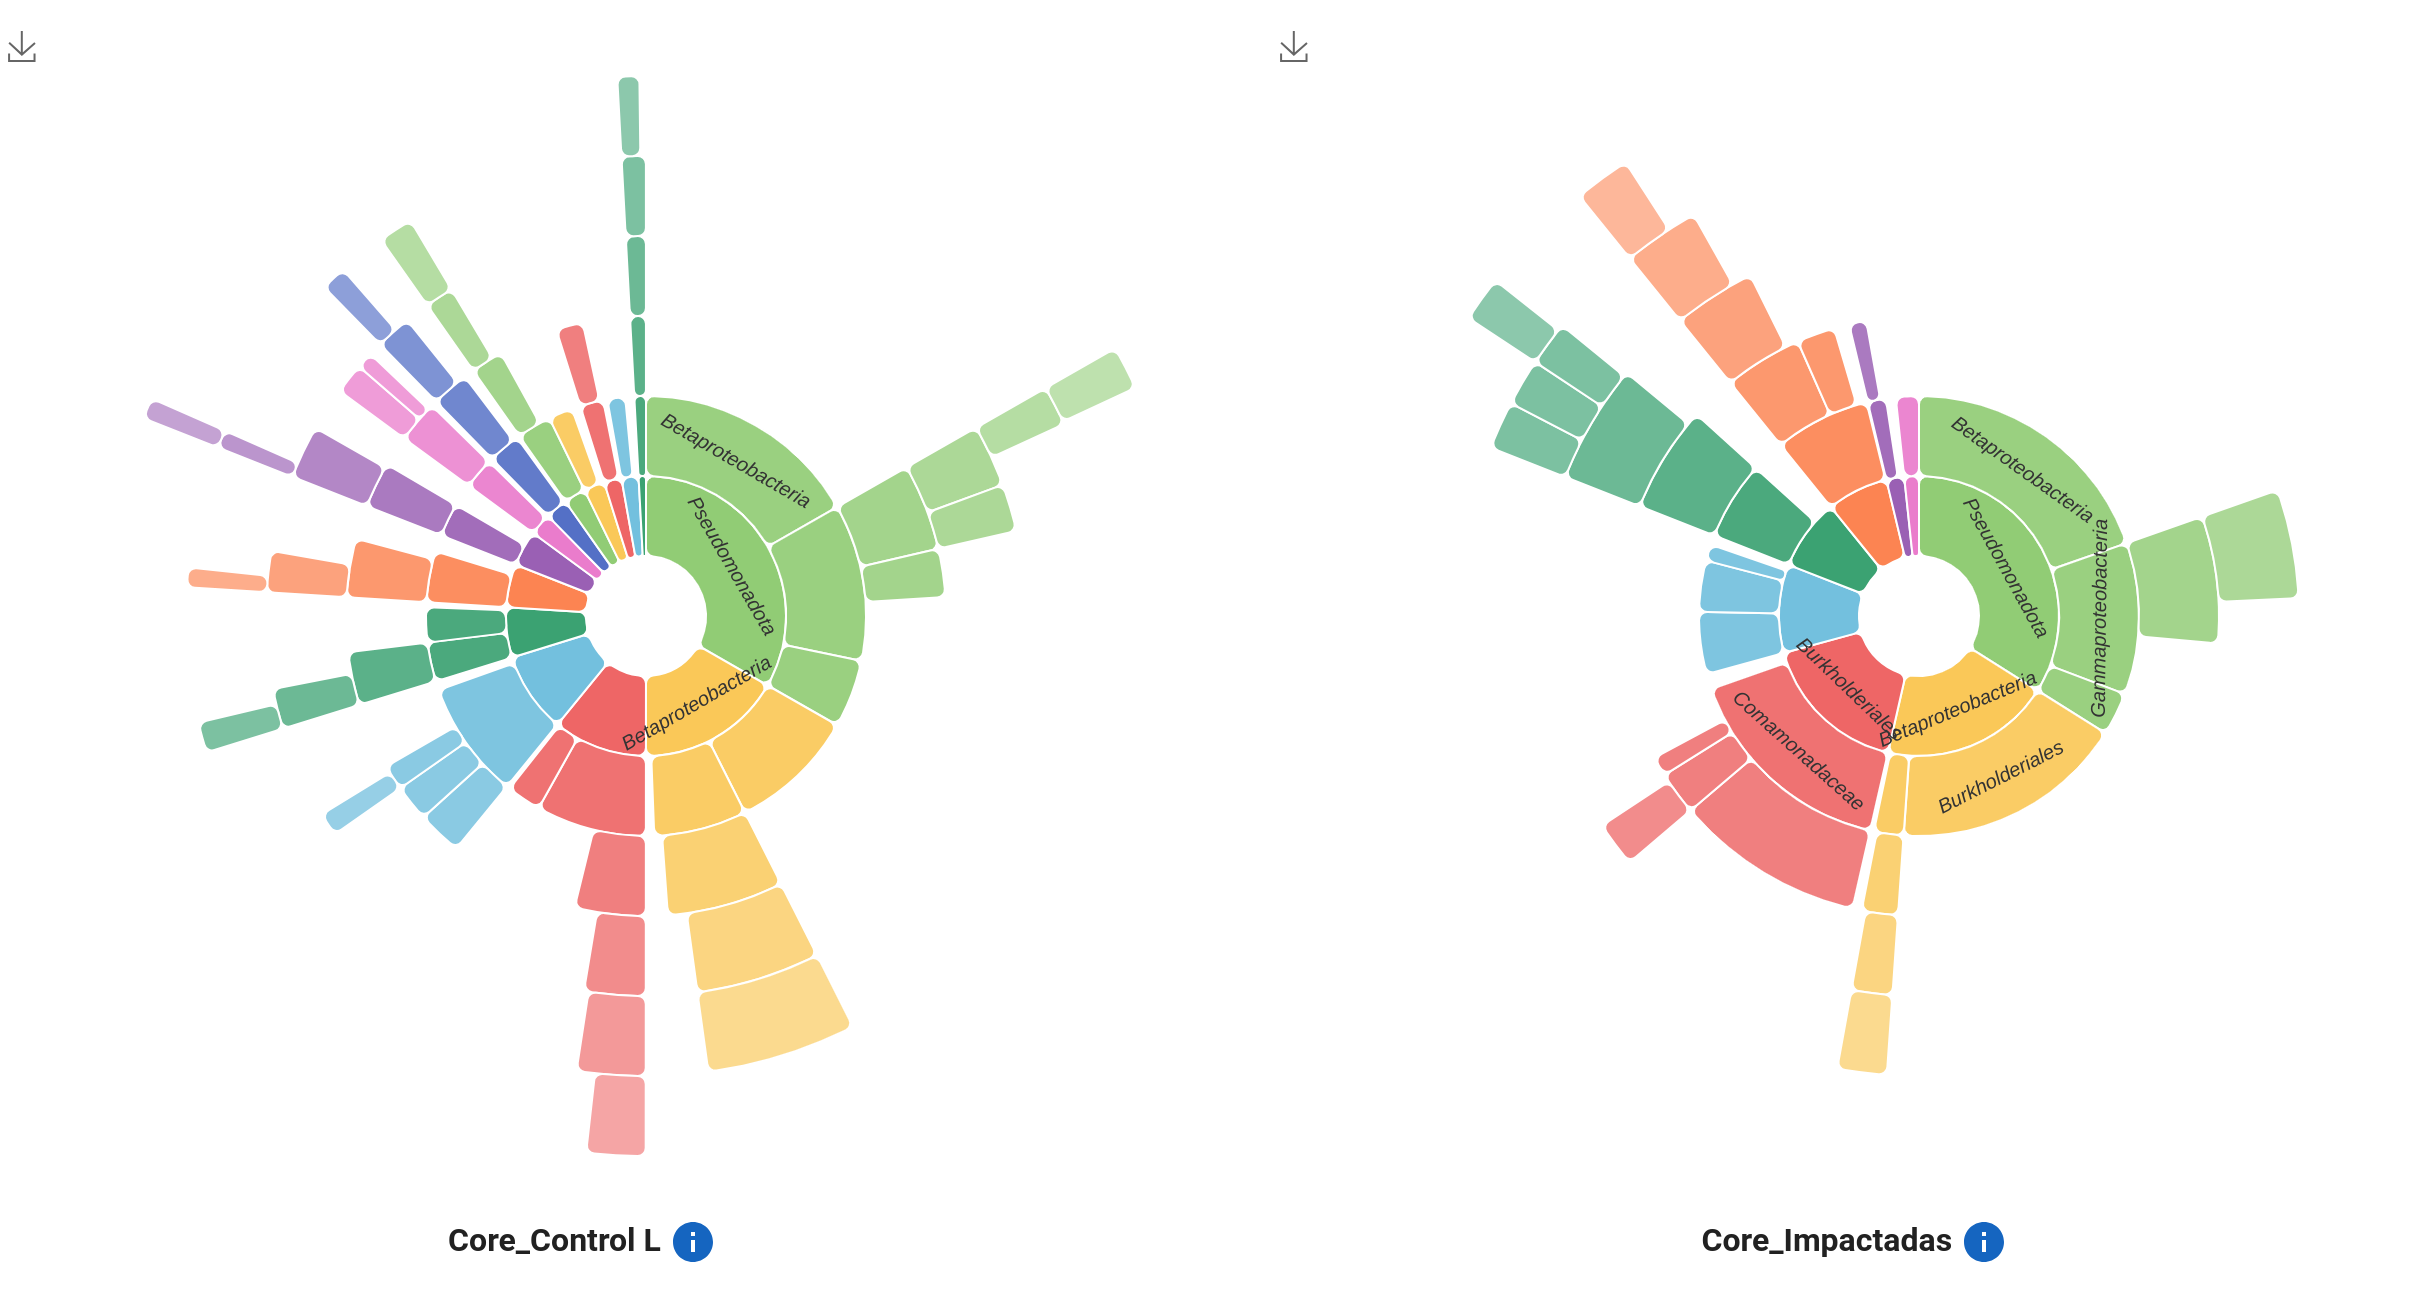
\includegraphics[width=0.8\linewidth]{images/app/results/core.png}
%     % \captionsetup{justification=raggedright, width=0.45\linewidth, singlelinecheck=off}

%     % \captionsetup{width=0.45\linewidth}
%     \caption{Gráfico de similitud  (resultados)}
%     \label{fig:app-results-core}
% \end{figure}

% En esta sección se puede presentar un solo gráfico de las taxonomías compartidas entre todas las muestras, y en el caso de que el usuario haya ingresado grupos, se desplegaran además los gráficos por cada grupo, como se visualiza en la Figura~\ref{fig:app-results-core}.

% En la parte inferior del gráfico, al lado derecho de la leyenda se puede visualizar un icono, el cual al posicionarse sobre el, va a mostrar las muestras utilizadas para generar el gráfico(Figura~\ref{fig:app-results-core-tooltip}).

% \begin{figure}[H]
%     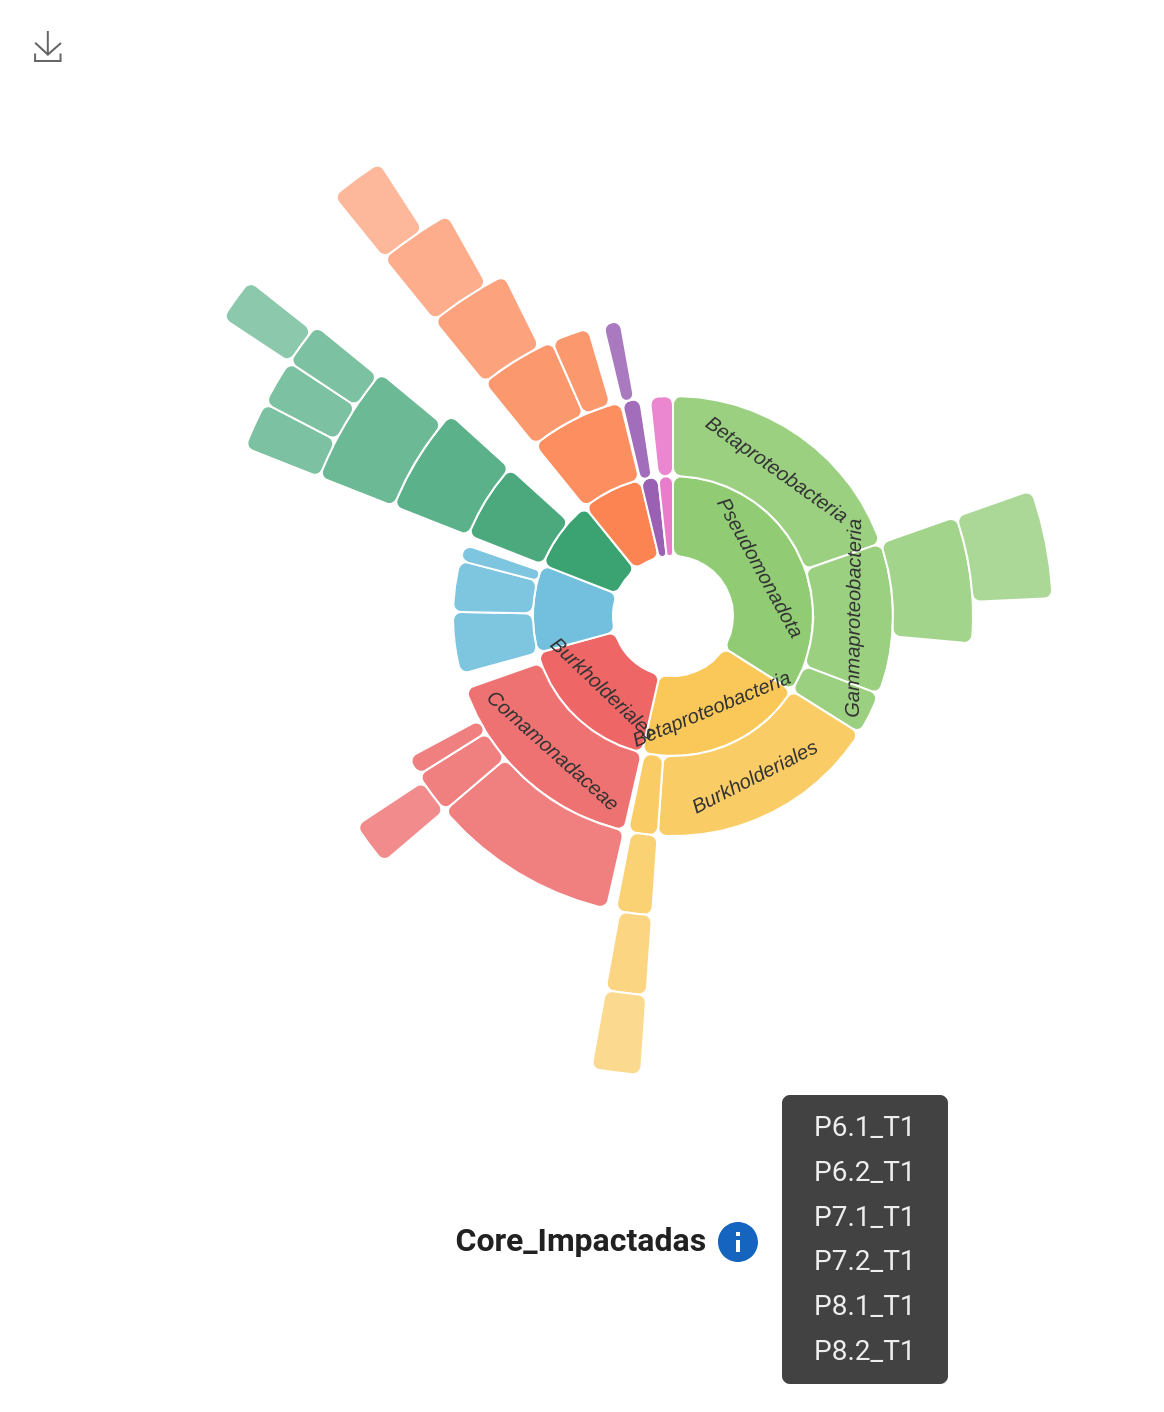
\includegraphics[width=0.8\linewidth]{images/app/results/core_tooltip.png}
%     % \captionsetup{justification=raggedright, width=0.45\linewidth, singlelinecheck=off}

%     % \captionsetup{width=0.45\linewidth}
%     \caption{Gráfico de similitud: Tooltip asociado a las muestras (resultados)}
%     \label{fig:app-results-core-tooltip}
% \end{figure}

% \subsection{Indices de diversidad}

% En caso de que el usuario hubiera ingresado grupos al inicio del proyecto y hubiera activado los análisis de índices de diversidad, se podrá visualizar tres gráficos boxplot, uno por cada índice de diversidad (Shannon, Simpson y Chao2). En caso de que el usuario no haya ingresado grupos, esta sección no se desplegará en la plataforma.

% A continuación se presenta un ejemplo de la visualización de esta sección en la plataforma:



% \subsection{Predicción funcional}
% Al igual que en la sección de asignación taxonómica, en la parte superior se pueden visualizar tres pestañas \textit{EC, KO y Pathways} que representan cada categoría funcional. Por defecto se presenta la información para la categoría de \textit{Pathways}.

% En la parte inferior izquierda se puede visualizar una tabla con la información de la predicción funcional obtenida mediante PICRUSt2 (EC, KO y Pathways) para cada muestra. 
% En la parte superior de la tabla se puede visualizar un campo de texto de búsqueda con el cual el usuario puede filtrar la información de la tabla.

% En el lado derecho de la sección, en caso de que el usuario hubiera ingresado grupos, se puede ver un gráfico de barras horizontales que muestra los pathways con diferencias significativas entre los grupos (información obtenida mediante LEfSe). 
% En caso de que no se haya ingresado información de grupos, solo se desplegará la tabla.

% Al igual que en la sección de asignación taxonómica el usuario puede interactuar con las pestañas modificando el contenido de las tablas mediante la selección de las pestañas.


% \begin{figure}[H]
%     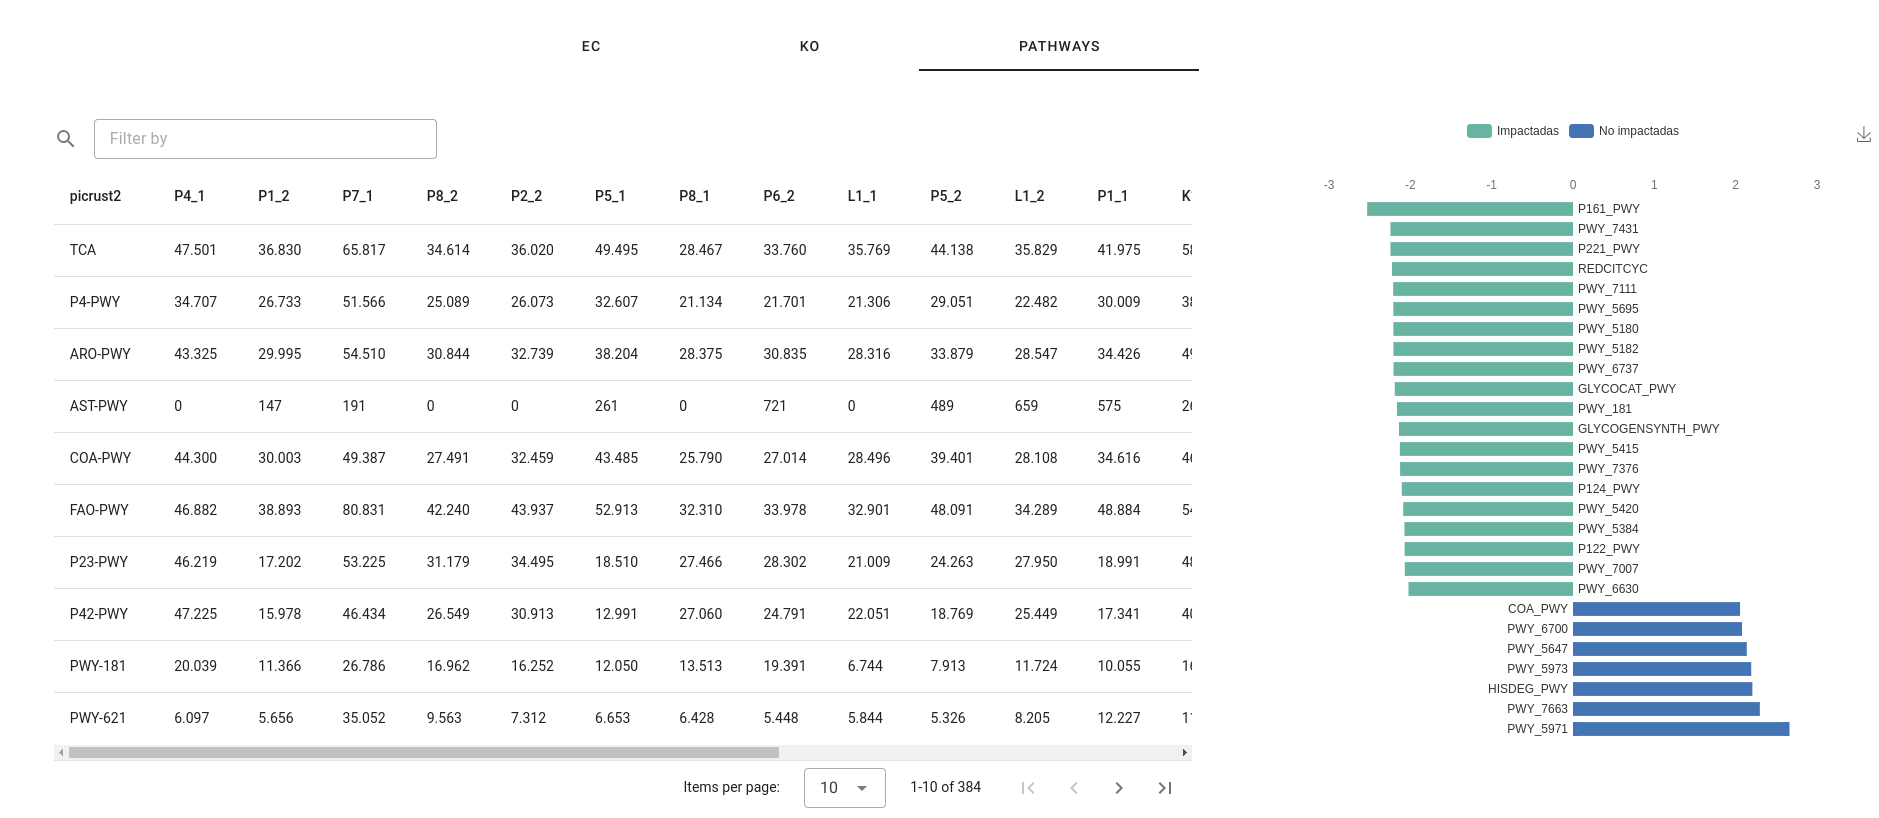
\includegraphics[width=1\linewidth]{images/app/results/functinoal_pred.png}
%     % \captionsetup{justification=raggedright, width=0.45\linewidth, singlelinecheck=off}

%     % \captionsetup{width=0.45\linewidth}
%     \caption{Resultados de predicción funcional: Tabla obtenida mediante PICRUSt2 y gráficod de diferencias significativas obtenido mediante LefSE}
%     \label{fig:app-results-functional-pred}
% \end{figure}
% \subsubsection{Descarga de los resultados}
% En la parte superior derecha de la sección de resultados, se encuentra un botón con el texto \textit{Download data}. 
% Al hacer click en este botón se descargará un archivo comprimido con toda los resultados generados por el pipeline.
% A continuación se detallan los archivos:
% \begin{itemize}
%     \item CSV de asignación taxonomica por muestra y por grupo (en caso de ingresarse), y por porcentaje y cantidad de lecturas
%     \item CSV de predicción funcional (EC, KO y pathways), en caso de haber seleccionado predicción funcional dentro de los análisis.
%     \item CSV con los valores del cálculo de los indices de diversidad
%     % \item \hl{PDF con los gráficos de barras apiladas, Sunburst y boxplot}
%     % \item \hl{Archivo de texto con la información del pipeline (versión, parámetros, etc)}
% \end{itemize}


% \begin{figure}[H]
%     
\includegraphics[width=1\linewidth]{images/app/donwload_button.png}
%     % \captionsetup{justification=raggedright, width=0.45\linewidth, singlelinecheck=off}

%     % \captionsetup{width=0.45\linewidth}
%     \caption{Gráfico de similitud: Tooltip asociado a las muestras (resultados)}
%     \label{fig:app-download-button}
% \end{figure}

% % \begin{figure}[H]
% %     \includegraphics[width=1\linewidth]{images/app/results/downloadbutton.png}
% %     % \captionsetup{justification=raggedright, width=0.45\linewidth, singlelinecheck=off}

% %     % \captionsetup{width=0.45\linewidth}
% %     \caption{Botón de descarga de resultados(resultados)}
% %     \label{fig:app-results-download}
% % \end{figure}

% \subsection{Integración del flujo de trabajo y aplicación web}

% Se diseñó una base de datos no relacional utilizando PostgreSQL.
% Esta base de datos permite almacenar la información de los proyectos subidos por el usuario en la plataforma web y los resultados obtenidos al ejecutar el flujo de trabajo.
% La base de datos funciona como intermedio entre el flujo de trabajo y la base de datos, permitiendo que la aplicación web escriba la metadata asociada al proyecto para que el flujo de trabajo pueda ejecutarse, y permitiendo además que la aplicación web pueda leer los resultados escritos por el flujo de trabajo, para poder convertir esta información en tablas y gráficos que permitan al usuario visualizar los resultados de manera sencilla.

% La base de datos esta compuesta por siete tablas:
% \begin{itemize}
%     \item PlatformRoles: Almacena los roles de la plataforma (admin, basic user).
%     \item Users: Almacena la información de los usuarios registrados en la plataforma.
%     \item Projects: Almacena la información de los proyectos subidos por los usuarios.
%     \item ProjectRoles: Almacena los roles de los usuarios dentro de los proyectos. Esto permite que un projecto y sus resultados puedan ser visualizados por varios usuarios a la vez.
%     \item ProjectRolesUsers: Almacena la relación entre los usuarios y los roles de los proyectos. Permitiendo a los usuarios tener diferentes roles en diferentes proyectos (solo lectura, edición, eliminar).
%     \item Results: Almacena los resultados obtenidos en la ejecución del flujo de trabajo.
%     \item PipelineDefaultParams: Almacena los parámetros por defecto de cada versión del flujo de trabajo.
% \end{itemize}

% \begin{figure}[H]
%     \centering
%     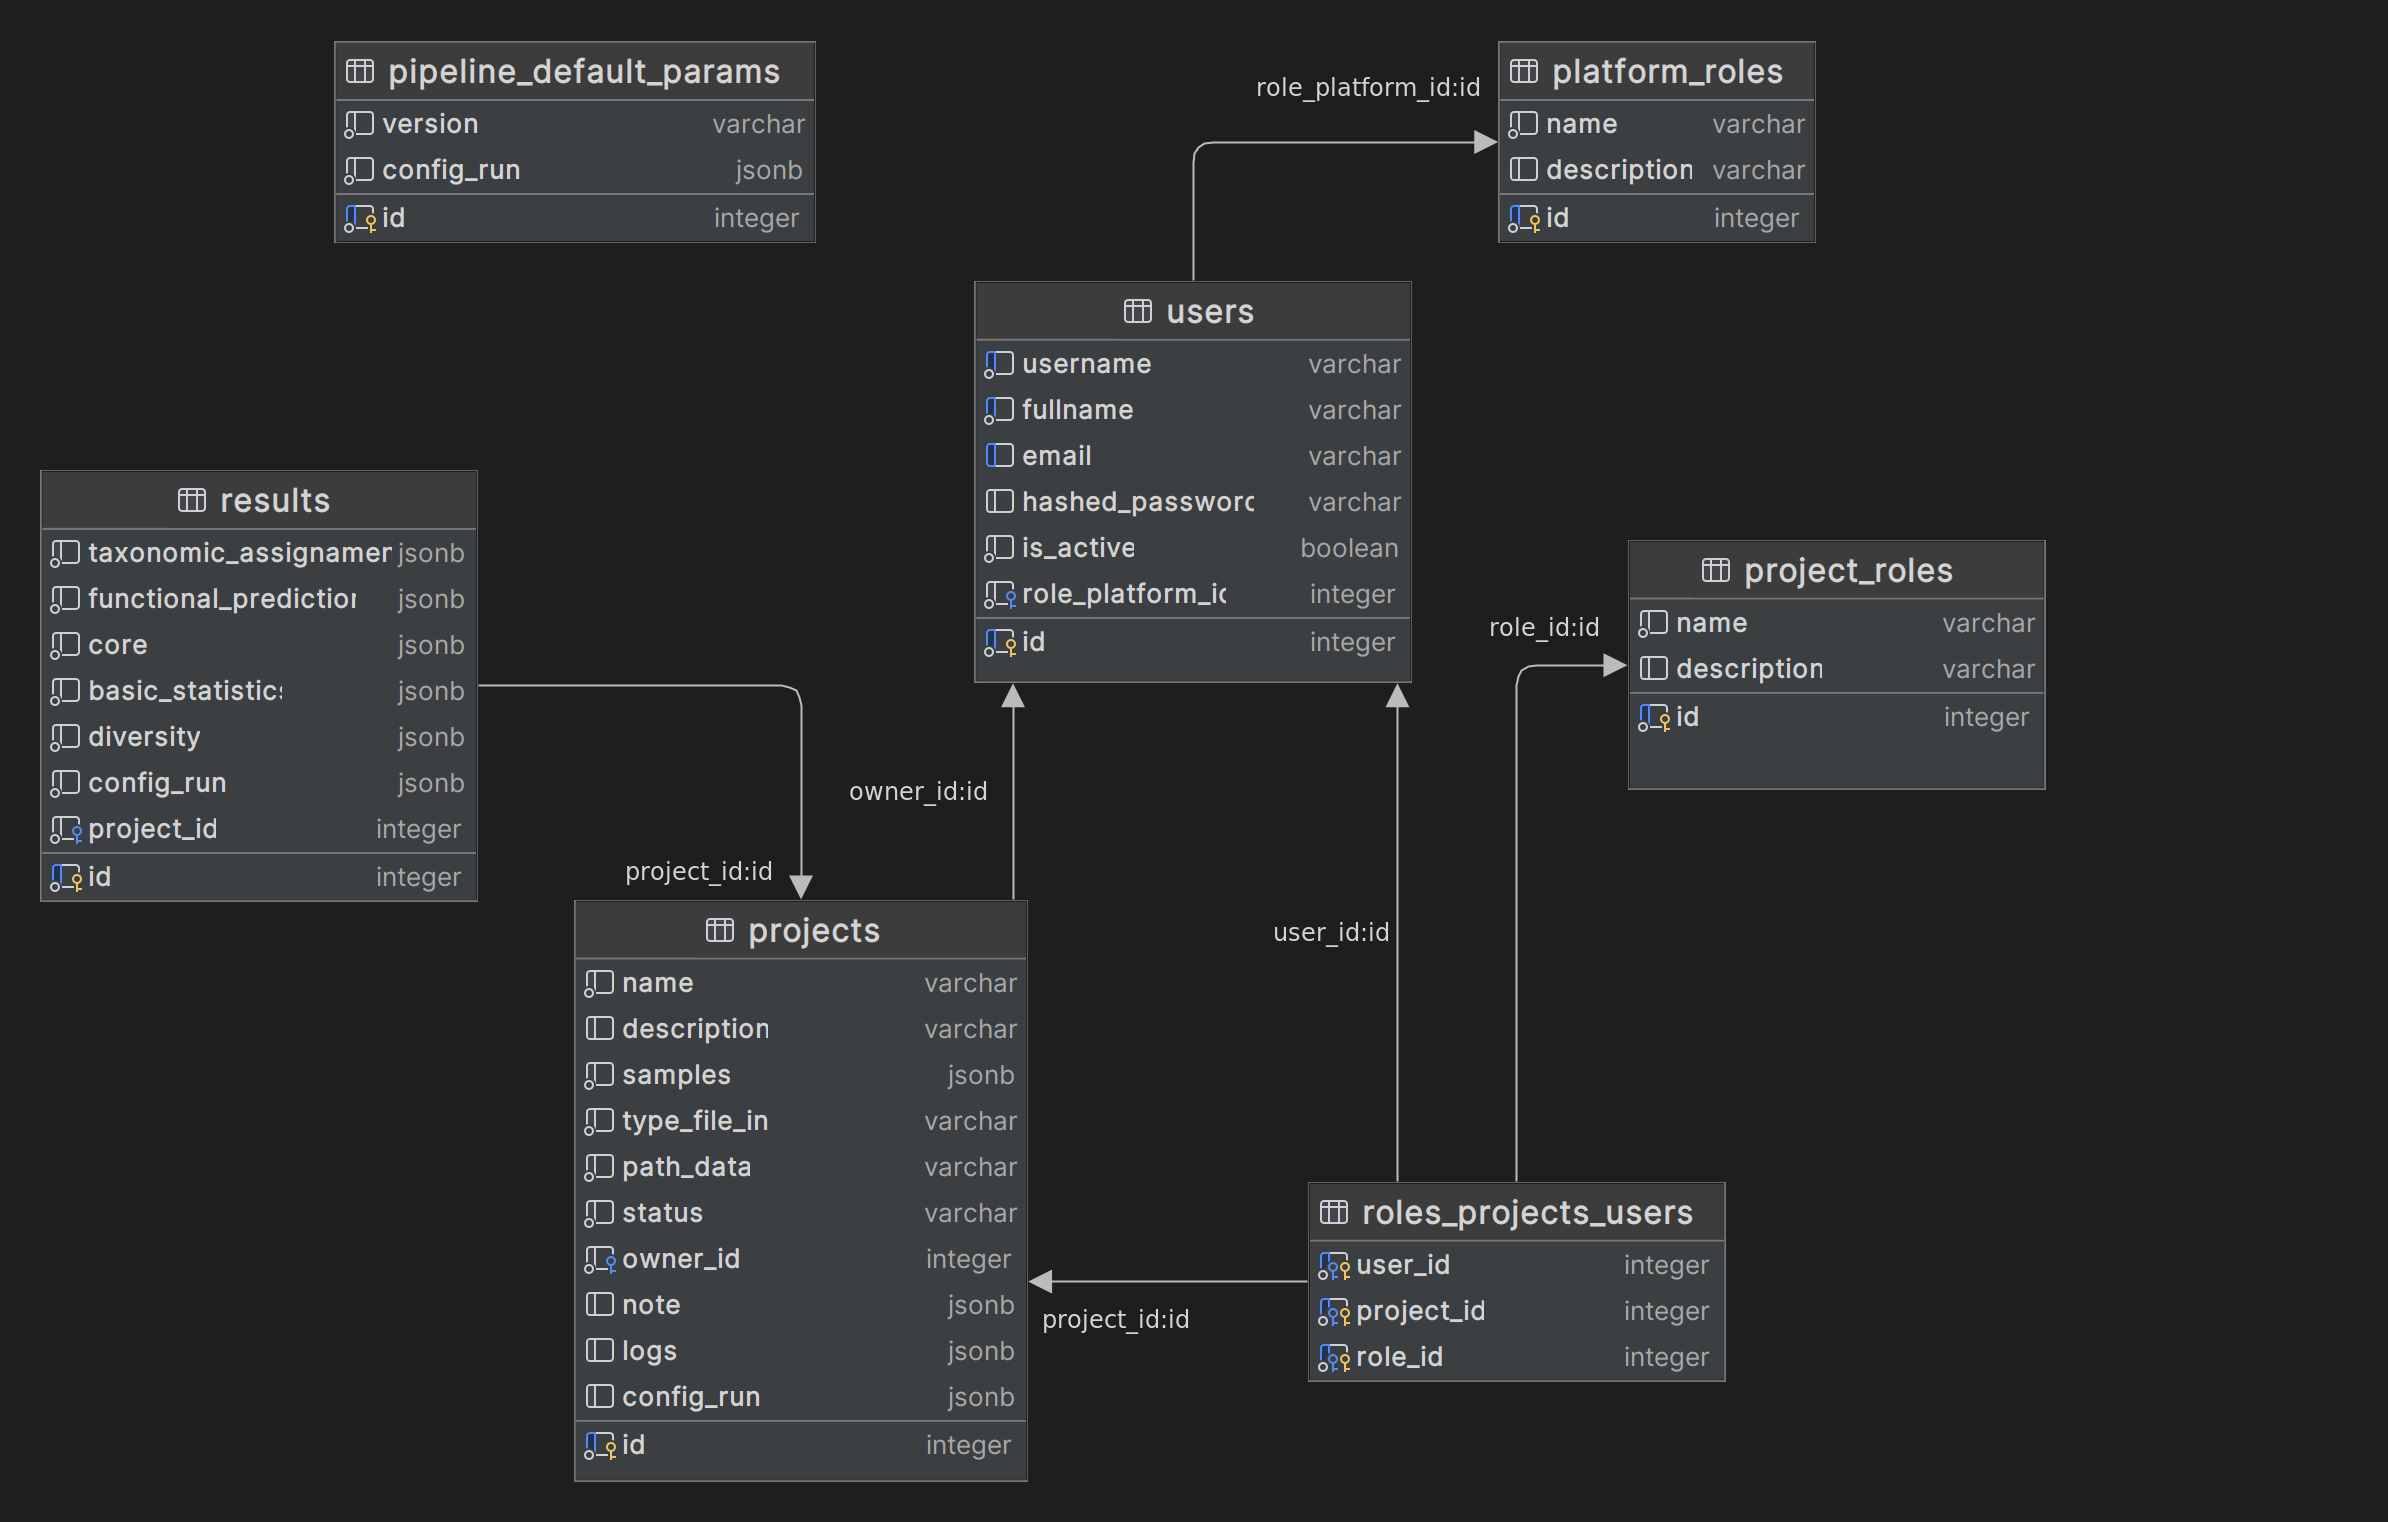
\includegraphics[width=1\linewidth]{images/dbb.png}
%     \caption{Base de datos}
%     \label{fig:nanotax-db}
% \end{figure}

% Las tablas de Resultados y Proyectos estan compuestas por campos JSONB que permiten almacenar datos en formato JSON mediante una representación binaria permitiendo que los datos sean indexados y consultados de manera eficiente. 

% Para la ejecución del flujo de trabajo se desarrollo un script en Python que escribe el archivo \textit{params.yml} con la información del proyecto y los parámetros ingresados por el usuario en la plataforma (y guardados en la base de datos).
% Una vez que el pipeline finaliza su ejecucción mediante un script en Python se almacenan los resultados en la base de datos.

% \subsection{Documentación}
% En esta sección se despliega la documentación del pipeline, la cual cuenta con la información de los módulos, parámetros y herramientas utilizadas en el pipeline. La documentación se encuentra dividida por cada módulo, donde se muestra la versión de la herramienta utilizada y los parámetros por defecto y modificables por el usuario.
% \subsubsection{Basecalling y demultiplexación}
% \subsubsection{Control de calidad}
% \subsubsection{Asignación taxonómica}
% \subsubsection{Predicción funcional}
% \subsubsection{Indices de diversidad}

